\documentclass[master]{BYUPhys}
% % These packages typeset the thesis with Times Roman font
% \usepackage[T1]{fontenc}
% \usepackage{textcomp}
% \usepackage{mathptmx}

%I love these packages.
\usepackage{amsmath}
\usepackage{amssymb}



% Allow the inclusion of graphics
\usepackage{graphicx}

% The fancyhdr package allows you to easily customize the page header.
% The settings below produce a nice, well separated header.
\usepackage{fancyhdr}
  \fancyhead{}
  \fancyhead[LO]{\slshape \rightmark}
  \fancyhead[RO,LE]{\textbf{\thepage}}
  \fancyhead[RE]{\slshape \leftmark}
  \fancyfoot{}
  \pagestyle{fancy}
  \renewcommand{\chaptermark}[1]{\markboth{\chaptername \ \thechapter \ \ #1}{}}
  \renewcommand{\sectionmark}[1]{\markright{\thesection \ \ #1}}

% The caption package allows you to change the formatting of figure captions.
% The commands here change to the suggested caption format: single spaced and a bold tag
\usepackage[margin=0.3in,labelfont=bf,labelsep=none]{caption}
 \DeclareCaptionFormat{suggested}{\singlespace#1#2 #3\par\doublespace}
 \captionsetup{format=suggested}


% The cite package cleans up the way citations are handled.  For example, it
% changes the citation [1,2,3,6,7,8,9,10,11] into [1-3,6-11].  If your advisor
% wants superscript citations, use the overcite package instead of the cite package.
\usepackage{cite}

% The makeidx package makes your index for you.  To make an index entry,
% go to the place in the book that should be referenced and type
%  \index{key}
% An index entry labeled "key" (or whatever you type) will then
% be included and point to the correct page.
\usepackage{makeidx}
\makeindex

% If you have a lot of equations, you might be interested in the amstex package.
% It defines a number of environments and macros that are helpful for mathematics.
% We don't do much math in this example, so we haven't used amstex here.

% The hyperref package provides automatic linking and bookmarking for the table
% of contents, index, equation references, and figure references.  It must be
% included for the BYU Physics class to make a properly functioning electronic
% thesis.  It should be the last package loaded if possible.
%
% To include a link in your pdf use \href{URL}{Text to be displayed}.  If your
% display text is the URL, you probably should use the \url{} command discussed
% above.
%
% To add a bookmark in the pdf you can use \pdfbookmark.  You can look up its usage
% in the hyperref package documentation
\usepackage[bookmarksnumbered,pdfpagelabels=true,plainpages=false,colorlinks=true,
            linkcolor=black,citecolor=black,urlcolor=blue]{hyperref}
\urlstyle{rm}
% ------------------------- Fill in these fields for the preliminary pages ----------------------------
%
% For Senior and honors this is the year and month that you submit the thesis
% For Masters and PhD, this is your graduation date
  \Year{2015}
  \Month{June}
  \Author{James Lawrence Archibald II}

% If you have a long title, split it between two lines using the \\ command.
% A multiple line title should be an "inverted pyramid" with the top line(s) longer than the bottom.
  \Title{Construction of a 408 nm Laser System \\ for use in Ion Interferometry}

% Your research advisor
  \Advisor{Dallin S. Durfee}

% The text of your abstract
  \Abstract{We discuss the construction of a 408 nm laser system for use in a $^{87}$Sr+ ion interferometer. The laser system produces two coupled beams with a 5 GHz relative detuning that are designed to stimulate Raman transitions between the $F=4$ and $F=5$ $^2$S$_{1/2}$ states of $^{87}$Sr+ using the $^2$P$_{3/2}$ state as the intermediate state. We present a detailed explanation of the design and construction of the laser system and calculations of the transition rate between the two states.}

 \Keywords{Sr, ion interferometer, photon rest mass, laser, AOM}

% Acknowledge those who helped and supported you
  \Acknowledgments{Camille has been a wonderful support. 
  }

\fussy
\DeclareMathOperator{\erf} {erf}


%\includeonly{AOMinstall}
%\includeonly{historicalOverviewAndMotivation}
%\includeonly{triumphantData}
%\includeonly{theAtoms}

\begin{document}
\frontmatter

\makepreliminarypages

\singlespace

\tableofcontents
\clearemptydoublepage

\listoffigures
\clearemptydoublepage

\doublespace


\newcommand{\includeorput}[1]{\include{#1}} %\newcommand{\includeorput}[1]{\input{#1}}
\mainmatter


\chapter{Background}
In this chapter, we discuss the overall experiment of which the 408 nm 5 GHz detuned laser system is a part. We will give a detailed summary of the preparation the atoms undergo before they are exposed to our laser system. We will also attempt to sensibly contextualize the ion interferometer vis-\`a-vis other physics experiments. 

\section{Ion Interferometer Basic Overview}
The ion interferometer uses a Mach-Zehnder configuration, which refers to the fact that it relies on splitting and recombining the interfering beam of atoms. See Fig.\ \ref{mach-zehnder-fig}. 


\begin{figure}
\centerline{
\includegraphics[width=0.95\textwidth]{mach-zehnder}}
\caption[Optical and Matterwave Mach Zehnder interferometers]{\label{mach-zehnder-fig}A traditional realization of an optical Mach Zehnder interferometer (top) juxtaposed with a sparse diagram of the ion interferometer (bottom). The ion interferometer is designed to achieve interference of matter waves and uses continuous wave lasers as its beam splitters. Notice that both involve splitting and recombining the beam. }
\end{figure}


As with any interferometer, the essential feature is that there is travelling wave that is split and sent along two paths. The output of the interferometer gives information about the relative phase shift acquired along each of the arms of the interferometer. 

The crucial feature of any interferometer is the splitting and recombining of waves in such a way that the relative phase difference between the two paths may be indirectly observed. In our interferometer, we plan to achieve interference of the atomic wave function of our $^{87}$Sr$^+$ ions. 
In order to accomplish ion interferometry, we must first acquire a suitable source of $^{87}$Sr$+$ ions. 

Thus, there are three basic steps associated with the operation of the interferometer. 
\begin{itemize}
\item Generation of a low velocity beam of cold Strontium atoms   
\item Ionization 
\item Atom interferometry
\end{itemize} 

The basic outline of the apparatus is illustrated in Figure~\ref{fig:IonInterferometer}.

\begin{figure}
\centerline{
\includegraphics[totalheight=0.3\textheight]{interferometer_diagram}
}
\caption[Ion Interferometer]{\label{fig:IonInterferometer}
The entire Strontium interferometer. } 
\end{figure}

\section{Trapping of Neutral Strontium and Low Velocity Intense Source (LVIS)}

First, we must obtain a slow-moving beam of ionized $^{87}$Sr$+$. This is accomplished in two steps. 

We trap the $^{87}$Sr in a magneto-optical trap (MOT) using the standard techniques as outlined in Ref.\ \cite{cjeDiss}. 

The dominant cooling effect in the MOT is Doppler cooling. The trap consists of 6 red-detuned laser beams originating from the 460.8 nm laser system described in \cite{cjeDiss}. These point from each of six directions towards the center of the MOT. 

The 5s$^2$ $^1$S$_0$ to 5s5p $^1$P$_1$ transition is used to cool the atoms. This process selects the 87u isotope of Strontium \footnote{Further rejection of other Sr isotopes occurs because the Raman beams will not drive their transitions.}
The trapping is achieved using a pair of permanent rare-earth magnets. The Zeeman shift of the levels addressed by the the lasers traps them within a small range. The amount of trapped atoms is enhanced by our use of a Zeeman slower. 

We create an LVIS \cite{cjeDiss} following techniques developed by \cite{LVIS}. One of the mirrors in in the trap has a small hole drilled in it.\footnote{This hole was drilled in-house and the details of how we avoided damage and tests that verify the integrity of its optical surface can be seen in \cite{cjeDiss}} This allows some of the atoms to escape the trap. These atoms have a relatively narrow distribution of velocities. \footnote{Probably cite some other reference here--whoever invented/talked about the LVIS}

The atoms that drift out of the trap are then accelerated by a sort of Zeeman acceleration effect \footnote{i.e. the same as the effect exploited in a Zeeman slower, but they're not slowing down. The magnetic field gradients that cause this are created by the same magnets that are used to make the gradient in the middle of the trap.}

\section{Ionization of Strontium}
 
The next step is to selectively ionize the $^{87}$Sr to produce $^{87}$Sr$+$. This is accomplished using a pair of resonant transitions, which place the electron in a state in an autoionizing state whose energy is higher than the lowest energy states in the continuum. 

First, we stimulate the 5s$^2$ $^1$S$_0 \rightarrow$ 5s5p $^1$P$_1$ transition, which, conveniently, is the same 461 nm transition used to cool the atom. The second transition is the 5s5p $^1$P$_1\rightarrow$5p$^2$ $^1$D$_2$ transition. The $^1$D$_2$ state is 57 meV above the ionization threshold \cite{NSFprop}. This can be accomplished with a 408 nm laser. This can be achieved using GaN diode lasers \footnote{Maybe InGaN? It is the same diode laser technology used in Blu-ray players.}

\section{Acceleration of Beam}

The ions, which are at this point already travelling at some speed are then accelerated in an electric field produced by two pieces of copper held at constant potential. This gives us freedom to control the speed of the atoms. 


\section{Interferometry}

The interferometry is then achieved. 

%the waves that are interfered are the quantum mechanical matter waves of our atoms. I borrowed the words "atomic wave function" phrase from chu and kasevich

In order to produce two distinct paths, we uses stimulated Raman transitions as done by Ref.\ \cite{kasevichChu1991}. We use stimulated Raman transitions. This is a two photon process whereby we drive the atoms from one state to another using a third state as an intermediate state. We have 3 pairs of overlapping 408 nm lasers in our apparatus and each of these pairs is tuned to induce a stimulated Raman transition between the two $^2$S$_{1/2}$ ($5s$) ground states corresponding to $F=4$ and $F=5$. The transition uses the $^2$P$_{3/2}$ ($5p$) state as an intermediate state. 

%The stimulated Raman transition process is one whereby we 

The essential analysis will be saved for Chapter \ref{ChapterAboutTheAtoms}.


%trust yourself and know that you know it. and know that it doesn't have to be much better than it will be to be acceptable. 

%Is it true that at the end, we can distinguish between the F=4 and F=5 ground state of the Strontium? 
%I hope so. Those are the two states, haha. 





\chapter{Background}

\section{Basics of Ion Inteferometer}

This work includes an overview of ion interferometer experiment and a detailed exposition of the construction of the laser system that drives the stimulated Raman transitions. It also includes some calculations about it. 

The ion interferometer uses a Mach-Zehnder setup to achieve interferometry with $^{87}$Sr+ ions. There are thre basic steps involved: 
\begin{itemize}

\end{itemize}



Our setup uses 


\section{Historical Precedents}
In this section, we will discuss some related experiments as context for our experiment. This will include historical intellectual forebears and some more modern cousins. 
 \subsection{Interference effects involving light}
Matter interferometry borrows many of its foundational concepts and terminology from interferometric light experiments. 
The wave nature of light has been the subject of serious study for a long time (e.g. Newton's rings). Young's double slit experiment was important in illustrating this. Young placed two slits and passed light through them. He then observed a pattern of alternating dark and light fringes corresponding to the regions of constructive and destructive interference. This represents a species of interferometry since there are two possible paths and their result depends on the relative phase shift between them. 

The Michaelson-Morley interferometer 


The diffraction of light in this way is in fact directly analogous to the methods use in some matter-wave interferometry experiments. For example, Alex Kronin uses very small gratings to produce similar patterns \cite{Kronin_RMP}. 

DeBroglie hypothesized that matter exhibits wave-like behavior. Some of the earliest direct confirmation of this was achieved by Davisson and Germer, whose electron scattering experiment was directly analogous in interpretation to Bragg diffraction experiments performed using light. 

\subsection{Coherent Manipulation of Matter}
Matterwave interferometry arose with the development of techniques for the coherent control and measurement of atoms \cite{Kronin_RMP}. Rabi was among the first to use rf resonances to coherently control the internal states of molecules\footnote{I think this is right}. Ramsey's work in creating long-lived superpositions and the method of separate oscillatory fields was similarly seminal \cite{Kronin_RMP}. 
More recently, atom interferometers have been used for many different types of experiments. These have provided high-precision measurements of the fine structure constant \footnote{I'll have to find some citations. This is basically just a list of things I saw at conferences that I thought were cool}, investigations of gravitational effects and placed ever tighter limits on potential deviations from Standard Model physics. 
%\subsection{Charged Particle Atomic Physics}

\subsection{Laboratory-based electromagnetic tests}

One possible application of our apparatus is that it can be used  to detect small electric fields in a setup like the one famously used by Cavendish in his early electrostatic experiments. Cavendish effectively measured fundamental electrostatic constants by measuring the electric filed inside a charged, conducting enclosure. By demonstrating that the electric fields were 0 regarldless of the charge on the enclosure, Cavendish was able to deduce that the repulsion between like electric charges falls off in proportion to the inverse of the square of the distance between them. \footnote{todo: cite this guy later maybe:  http://geometrydude.wordpress.com/2012/12/22/cavendishs-phenomenological-derivation-of-coulombs-law/}. 

The ion interferometer is Our experiment is similar to Cavendish's experiment in two ways: First, one possible application of the ion interferometer is that it could be placed inside a conductive shell whose electric potential is varied. have a very similar setup as Cavendish's. The ion interferometer provides a sensitive way to measure electric fields inside a conducting shell that will be charged and discharged. 

The second way in which our experiment is related to Cavendish's is that it seeks to shed light on fundamental electromagnetic phenomena. Our our experiment seeks to measure fundamental electrical constants. Cavendish was able to measure the $1/r^2$ dependence in what eventually became known as Coulomb's law. Our experiment hopes to place a limit on the photon rest mass.\footnote{Our experiment will also produce results that may be reported as $\epsilon$ in the $1/r^{2+\epsilon}$ generalization of Coulomb's law.}
%footnote{who am I to say who did what first?}\cite{jackson} \footnote{it'd be nice to get Cavendish's original paper} 
%I don't really know if the finite conductivity of the shell matters for our experiment. 
%can we characterize copper in some way? I mean by taking time-dependent measurements of the dispersion of charge within the cavity? 
In fact, Cavendish's experiment directly inspired our experiment\footnote{This is a piece of lab oral history that I wanted to preserve}. Brian Neyenhuis, whose time working in Dallin's lab overlapped with mine, came across a practice GRE question about the best laboratory measurements to date confirming Coulomb's law. It turned out that these were a variation on Cavendish's method. They key limiting factor in all cases was the experimenter's ability to measure small electric fields inside the conducting shell. Brian started investigating the use of atomic physics techniques to improve these measurements. Soon he and Dallin had fleshed out their idea for creating an ion interferometer.  

According to Ref.\ \cite{jackson}. Many of the more recent tests of electrostatics were performed using setups similar to Cavendish's. 

%todo: find that paper that cites our experiment 
There are many other experiments along these lines as detailed in \cite{PhotonMassSurvey}. 

\subsection{More recent antecedent}
Electron interferometry using gratings has been achieved. \footnote{cite!!} Furthermore, ion interferometry has been achieved only using physical gratings. One of our experiment's main advantages is that its beamsplitters use no physical gratings

There are atomic clocks that use long-lived coherent superpositions of internal states of ions.\footnote{todo:cite}. However, The ions themselves do not enclose spacelike areas over the course of their path.

Coherent manipulation has also (thankfully!) been achieved in many labs \footnote{Todo:CITE!}. For example, neutral Sr has been trapped and cooled by XXXXX. 
Other experiments involving Sr TODO: add the other experiments.

The interest in $^{87}$Sr+ has been helpful not least because there are good numerical estimates of various transition parameters \cite{safronovaTheory}



\chapter{Laser Pieces}
%the sum of the whole is greater than the parts 

The laser system consists of several components arranged together on a breadboard. 

\begin{figure}
    \centerline{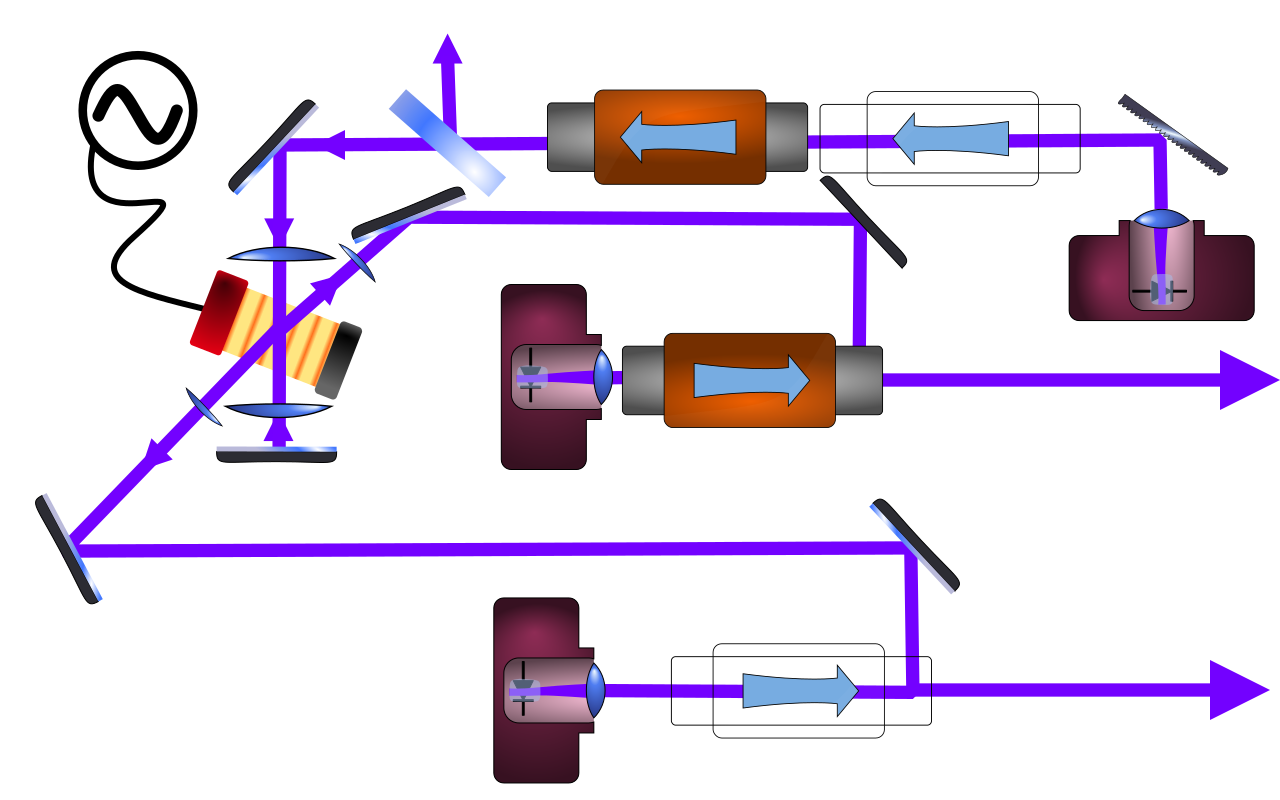
\includegraphics[width=1\textwidth]{diagramOfSetup3}}
    \caption[Numerical method]{\label{fig:diagramOfSetup}
    Just plot the magnitude of the vertically polarized component as a function of $\theta_1$. I used the slider to control $\theta_2$. Obviously, I'll illustrate this better at some point.}
\end{figure}


There are three separate laser diodes in housings. One of them is designated the "Master" laser. The master laser is grating stabilized using an extended cavity formed by a  %look this up
lines/mm diffraction grating mounted on a piezoelectric mount.  

The master laser passes through two optical isolators. It is then passed through a pair of waveplates and a polarizing beam cube, which serves the dual purpose of allowing us to attenuate the portion of the beam that goes through the AOM and splitting off a beam that can be used in our spectrum analyzer. 

After this, the laser is passed twice through an Acousto-optic Modulator (AOM). This splits off two beams, one of which is shifted upwards by 2.5 GHz and the other of which is shifted downward by 2.5 GHz. These two beams are then coupled through optical isolators into the two slave lasers. The outputs of these two lasers are what we use in our experiment to achieve stimulated Raman transitions. 



\chapter{The Atoms} \label{ChapterAboutTheAtoms}
%\section{Overview of relevant atomic transitions}

The objective of this chapter is to find the intensity and beam waist that will allow our lasers to impart the $\pi$ and $\pi/2$ pulses to the atoms as they make their way through the chamber. In order to show that the 408 nm 5 GHz detuned laser can provide the $\pi$ and $\pi/2$ pulses, one must first take a detailed look at the Raman transitions that the laser system is intended to stimulate.
The basic steps that will be explained in this chapter are as follows:
\begin{itemize}
\item Model the dynamics of a generic three state atom undergoing a Raman transition.
\item Identify the relevant contributions to the $^{87}$Sr$^+$ ions' Hamiltonian and show that it can be modeled as a three state system.
\item Find and interpret appropriate numerical values for relevant physical parameters in the Hamiltonian.
\item Calculate the intensity, width and polarization of our laser beams that will allow the laser to impart the $\pi$ and $\pi/2$ pulses to the atom. 
\end{itemize}
In this way I will show that the beams from this laser system will be able to accomplish their intended purpose.

\section{Dynamics of two- and three-state systems}\label{dynamicsSection}

First, we will model the dynamics of the system based on information found in Refs.\,\cite{Young1997363}, \cite{gustavsonThesis}, \cite{footAtomicPhysics}, \cite{cjeDiss} and \cite{RamanBeamSplit}. 
We will eventually model the atom as a three-state system that undergoes stimulated Raman transitions. During these transitions, the atom moves coherently between the ground and excited states. In appropriate limits, however, the three-state system undergoing Raman transitions can be shown to be equivalent to a two-state system undergoing Rabi oscillations between the ground and excited states. Therefore, we will first review Rabi flopping in a two state system, after which we will discuss the dynamics of a three-state system. 

\subsection{Two state Rabi oscillations}
\label{twoStateSection}
The first step to understanding the physics of the Raman transitions is to understand the dynamics of a two state atom. The dynamics of this system are well-known. Discussions of it can be found in many places, including Refs.\,\cite{cohenTannoudji}, \cite{demilleBudkerKimball}, and \cite{Young1997363}. The Hamiltonian for a two level atom under periodic perturbation from an electric field can be written as 
\begin{equation}
H = \hbar \omega_e |e\rangle\langle e| + \hbar \omega_g |g\rangle\langle g| - \mathbf{d}\cdot\mathbf{E},
\end{equation} 
where $\omega_e$ and $\omega_g$ are the frequencies of the excited and ground states respectively and $\mathbf{d}$ is the dipole moment operator. The excited state is shown as $|e\rangle$, while $|g\rangle$ represents the ground state. The electric field $\mathbf{E}$ is given by 
\begin{equation}
\mathbf{E} = \mathbf{E_0} \cos (\omega t + \phi).
\end{equation}
Here, $\mathbf{E_0}$ represents the electric field amplitude and direction, while $\omega$ is the angular frequency of the laser, $t$ is time and $\phi$ encapsulates the phase of the radiation.
We have followed the conventions selected in Ref.\,\cite{Young1997363}. 
These equations can be solved by moving into the interaction picture, applying the rotating wave approximation, and diagonalizing the resulting matrix to find its eigenvalues and eigenstates.

If we let 
\begin{equation}
|\Psi(t)\rangle = c_e(t)e^{-i\omega_e t}|e\rangle + c_g e^{-i\omega_g t}|g\rangle
\end{equation}
represent the Schr\"odinger picture solution to the equation, then the solution in the case where $c_g(0)=1,c_e(0)=0$ turns out to be 
\begin{align}
c_e(\tau)&=-i e^{-i(\delta \tau/2+\phi)} \frac{\Omega_{eg}}{\Omega_{r}} \sin\left(\frac{\Omega_r \tau}{2}\right)\label{eqn:ce2stateRabi}\\
c_g(\tau)&=e^{i(\delta \tau/2)} \left(
\cos\left(\frac{\Omega_r \tau}{2}\right)
- i\frac{\delta}{\Omega_r} \sin\left(\frac{\Omega_r \tau}{2}\right)\right)
\label{eqn:cg2stateRabi},
\end{align}
where $\Omega_{eg}$ represents the on-resonance Rabi frequency, which is defined as 
\begin{equation}
\Omega_{eg}=-\frac{\langle e |\mathbf{d}\cdot\mathbf{E}|g \rangle }{\hbar}
\end{equation}
and the off-resonance Rabi frequency, $\Omega_r$, is defined as 
\begin{equation}
\Omega_r=\sqrt{\Omega_{eg}^2+\delta^2}.
\end{equation}
The detuning, $\delta$, is defined as 
\begin{equation}
\delta=\omega-(\omega_e-\omega_g).
\end{equation}
Equations\,\ref{eqn:ce2stateRabi} and \ref{eqn:cg2stateRabi} can be squared to find the total likelihood of finding the system in a particular state as a function of time (or, alternatively, we can interpret this as the population of the upper and lower states as a function of time):
\begin{align}
|c_e(\tau)|^2&=\left(\frac{\Omega_{eg}}{\Omega_r}\right)^2 \sin^2\left(\frac{\Omega_r\tau}{2}\right)
=\frac{\Omega_{eg}^2}{2\Omega_r^2}(1-\cos(\Omega_r\tau))\\
|c_g(\tau)|^2&=1-\left(1-\frac{\delta^2}{\Omega_r^2}\right)\sin^2
\left(\frac{\Omega_r \tau}{2}\right)
=1-\frac{\Omega_{eg}^2}{2\Omega_r^2} + \left(\frac{\Omega_{eg}^2}{2\Omega_r^2}\right)\cos(\Omega_r \tau).
\end{align}
%should I put \Omega_r^2 just to see? No. 
These results are also quoted from Ref.\,\cite{Young1997363}, whose conventions I have also adopted.

The two state Rabi system has some important properties. First, we see that the only way to move 100\% of the population from the ground state to the excited state is to drive the system on-resonance (i.e. with $\delta=0$). Second, we see that the system oscillates between populating the excited and ground states with frequency $\Omega_{r}$. The stronger the coupling between the laser and the system (which is encapsulated in $\langle e|\mathbf{d}\cdot\mathbf{E}|g\rangle$), the more rapidly these oscillations occur. 
\subsubsection{$\pi$ and $\pi/2$ pulses}
We are particularly interested in coherently swapping the entire populations of the two states and placing the ions into an equal, coherent superposition of the two states.
An interaction that coherently moves the system from one state to the other is called a $\pi$ pulse. An interaction that takes the system in one state into an equal superposition of the two states is caled a $\pi/2$ pulse. This terminology comes from the Bloch sphere. In the Bloch sphere, a superposition of $|e\rangle$ and $|g\rangle$ can be represented to within an overall phase as 
\begin{equation}
%|e\rangle\rightarrow \frac{1}{\sqrt{2}}\left(|e\rangle+e^{i\phi_{}}|g\rangle\right)
\cos\left(\frac{\theta}{2}\right)|g\rangle+
e^{i\phi}\sin\left(\frac{\theta}{2}\right)|e\rangle,
\end{equation}
where $\phi$ and $\theta$ are arbitrary angles that can be changed to represent any state. A $\pi/2$ pulse changes $\theta$ by $\pi/2$ radians, while a $\pi$ pulse changes it by $\pi$ radians.

There is a little more that we can say about these pulses. In the experiment, we would like a $\pi/2$ interaction with the laser to be able to take an ion in the $|g\rangle$ or $|e\rangle$ states and put it into an equal superposition of the $|g\rangle$ and $|e\rangle$ states. However, we would also like to be able to use the same pulse to take ions that are in equal superpositions of the $|e\rangle$ and $|g\rangle$ states and put them into either the ground or excited states.

We let $A$ be an operator representing a $\pi/2$ pulse that satisfies the above properties. Then the effect of $A$ on a state $|g\rangle$ is given by 
\begin{equation} \label{ppu1}
A|g\rangle = \frac{e^{i\phi_o}}{\sqrt{2}} \left(|g\rangle + e^{i\phi_e}|e\rangle\right),
\end{equation}
where $\phi_o$ and $\phi_e$ in this equation represent arbitrary constants.
%\begin{equation}
%\Pi=e^{i\phi_{eg}}|e\rangle\langle g|+e^{i\phi_{ge}}|g\rangle\langle e|,
%\end{equation}
%where $\phi_{eg}$ and $\phi_{ge}$ are arbitrary phases. 
%with some phase? shoot. 
Now, if we apply $A$ again, we would like to have 100\% of the population moved to the excited state (i.e. $A^2$ is equivalent to a $\pi$ pulse ): 
\begin{equation}
A^2|g\rangle = e^{i\phi_e'}|e\rangle\\
\end{equation}
Now, substituting the result of Eq.\,\eqref{ppu1}, we get
\begin{equation}
A\frac{e^{i\phi_o}}{\sqrt{2}} \left(|g\rangle + e^{i\phi_e}|e\rangle\right)=e^{i\phi_e'}|e\rangle.
\end{equation}
We can use the result of Eq.\,\eqref{ppu1} again to get 
\begin{equation}
\frac{e^{2i\phi_o}}{2}
|g\rangle
+
\frac{e^{i(2\phi_o+\phi_e)}}{2} |e\rangle
+
\frac{e^{i(\phi_o+\phi_e)}}{\sqrt{2}}
A|e\rangle
=e^{i\phi_e'}|e\rangle.
\end{equation}
We can solve this equation to find $A|e\rangle$: 
\begin{align}
A|e\rangle&= 
\frac{\sqrt{2}}{e^{i(\phi_o+\phi_e)}}
\left(
-\frac{e^{2i\phi_o}}{2}|g\rangle
+\left(e^{i\phi_e'}-\frac{e^{i(2\phi_o+\phi_e)}}{2}\right) |e\rangle
\right)\\
A|e\rangle&= 
-\frac{e^{i(\phi_o-\phi_e)}}{\sqrt{2}}|g\rangle
+\left(\sqrt{2}e^{i(\phi_e'-\phi_e-\phi_o)}-\frac{e^{i\phi_o}}{\sqrt{2}}\right) |e\rangle. \label{Aemidddle}
\end{align}
Since $A$ preserves normalization, we know that the sum of the norms of the coefficients of $|e\rangle$ and $|g\rangle$ must be one. Therefore, 
\begin{equation}
\left|-\frac{e^{i(\phi_o-\phi_e)}}{\sqrt{2}}\right|^2 + \left|\sqrt{2}e^{i(\phi_e'-\phi_e-\phi_o)}-\frac{e^{i\phi_o}}{\sqrt{2}}\right|^2 = 1.
\end{equation}
From this, we can solve to find that  
\begin{equation}
\cos\left(\phi_e'-\phi_e-2\phi_o\right) = 1.
\end{equation}
Therefore, 
\begin{equation}
\phi_e'-\phi_e = 2\phi_o.\label{phiophie}
\end{equation}
By substituting Eq.\,\eqref{phiophie} into Eq.\,\eqref{Aemidddle}, we get
\begin{equation}
A|e\rangle = \frac{e^{i\phi_o}}{\sqrt{2}}\left(-e^{-i\phi_e}|g\rangle + |e\rangle \right).
\end{equation}
Now, we know how $A$ acts on both $|e\rangle$ and $|g\rangle$, but we would like to figure out when we can expect to be able to apply $A$ and get a transition from an equal superposition of $|e\rangle$ and $|g\rangle$ states to a pure $|e\rangle$ or $|g\rangle$ state. If we allow $A$ to act on an arbitrary superposition with coefficients $a_e$ and $a_g$, then we get 
\begin{equation}
A\left(a_g|g\rangle+a_e|e\rangle\right)= 
\frac{e^{i\phi_o}}{\sqrt{2}}
\left(
(a_g-a_e e^{-i\phi_e})|g\rangle +
(a_e+a_g e^{i\phi_e})|e\rangle 
\right).
\end{equation}
Thus, in order to get $A\left(a_g|g\rangle+a_e|e\rangle\right)=e^{i\gamma}|e\rangle$ (with $\gamma$ an arbitrary phase), 
%\begin{equation}
%\begin{array}{r@{\mskip\thickmuskip}1}
%a_e+a_ge^{i\phi_e} &= e^{i\gamma} \\
%a_g-a_e e^{-i\phi_e} &= 0 
%\end{array}
%\Rightarrow
%\begin{array}{r@{\mskip\thickmuskip}1}
%a_e+a_ge^{i\phi_e} &= e^{i\gamma} \\
%a_g-a_e e^{-i\phi_e} &= 0 
%\end{array}
%\end{equation}
\begin{equation}
\begin{aligned}
\frac{e^{i\phi_o}}{\sqrt{2}}\left(a_e+a_ge^{i\phi_e}\right) &= e^{i\gamma} \\
\frac{e^{i\phi_o}}{\sqrt{2}}\left(a_g-a_e e^{-i\phi_e}\right) &= 0 
\end{aligned}
\quad\implies\quad
\begin{aligned}
a_e&=\frac{e^{i(\gamma-\phi_o)}}{\sqrt{2}}\\
a_g&=\frac{e^{i(\gamma-\phi_o-\phi_e)}}{\sqrt{2}}.
\end{aligned}
\end{equation}
Similarly, to get $A\left(a_g|g\rangle+a_e|e\rangle\right)=e^{i\gamma}|g\rangle$,
\begin{equation}
\begin{aligned}
\frac{e^{i\phi_o}}{\sqrt{2}}\left(a_e+a_ge^{i\phi_e}\right) &= 0 \\
\frac{e^{i\phi_o}}{\sqrt{2}}\left(a_g-a_e e^{-i\phi_e}\right) &= e^{i\gamma} 
\end{aligned}
\quad\implies\quad
\begin{aligned}
a_g&=\frac{e^{i(\gamma-\phi_o)}}{\sqrt{2}}\\
a_e&=-\frac{e^{i(\gamma-\phi_o+\phi_e)}}{\sqrt{2}}.
\end{aligned}
\end{equation}
Thus, in order for a $\pi/2$ pulse to put ions that are already in a superposition into one state or the other, it must be the case that 
\begin{equation}
|a_e|^2=|a_g|^2=\frac{1}{2}.
\end{equation}
In addition, the phase difference between the two states determines whether we can put that superposition state into a single state.  

This is handy because at the end of the interferometer, we hope to be able to detect the accumulated phase difference between the two beams. The phase is related to everything. TODO: write down phase relationship. 
%One way to impart a $\pi$ pulse to the atomic system, would be to turn on the laser field for some finite amount of time such that the system undergoes half of one complete Rabi oscillation over the duration of the pulse. We can calculate the necessary length of such a pulse to be simply half of the period associated with the effective Rabi rate, or in other words $T = 2\pi/\omega$.
%Similarly, we are interested in $\pi/2$ pulses, which are laser pulses that cause the following type of transition:
%\begin{multline}
%%|e\rangle\rightarrow \frac{1}{\sqrt{2}}\left(|e\rangle+e^{i\phi_{}}|g\rangle\right)
%\cos\left(\frac{\theta}{2}\right)|g\rangle+
%e^{i\phi}\sin\left(\frac{\theta}{2}\right)|e\rangle\rightarrow 
%\cos\left(\frac{\theta+\pi/2}{2}\right)|g\rangle+
%e^{i\phi'}\sin\left(\frac{\theta+\pi/2}{2}\right)|e\rangle.\label{blochSpherepi2}
%\end{multline}
%In this equation, $\theta$ is a coordinate representing the inclination angle on the Bloch sphere. The symbols $\phi$ and $\phi'$ represent arbitrary phases. The entire equation is specified only to within an overall phase. This shows that systems that are in a state $|e\rangle$ or $|g\rangle$ will be placed in an equal superposition of other states, while if the system is already in an equal superposition, the entire population will be moved to either the $e\rangle$ or $|g\rangle$ states.
%As Eq.\,\eqref{blochSpherepi2} illustrates, this is called a $\pi/2$ pulse because it changes the state of the system into an equal superposition, which is represented by the angle of $\pi/2$ radians in the Bloch sphere description of a two state system. Also, similar to the case of the $\pi$ pulse, a $\pi/2$ pulse can be achieved simply by turning on a Rabi-flop-inducing stimulus for the appropriate time interval, which is $T/4$. 
%
%could I have just said ae+bg->a(e+g)+b(e-g)? Probably something like that. Oh, also, don't forget that the phase doesn't matter. 
%The system is most naturally talked about in the interaction picture. In order to do this, I divide the Hamiltonian into two pieces: 
%\begin{equation}
%H=H_0+V
%\end{equation} 
%
%where $H$ is the total Hamiltonian, $H_0=\hbar \omega_e |e\rangle\langle e| + \hbar \omega_g|g\rangle\langle g|$ is the Hamiltonian of the atom not including the contribution from the external electric field and $V=\mathbf{d}\cdot\mathbf{E}$ represents the part of the Hamiltonian that describes the interaction of the laser with the system. To do this, I must make the standard transformations to the interaction picture. I get \cite{merzbacher} \cite{sakurai}, 
%
%\begin{align}
%|\psi\rangle_I &= e^{i H_0 t/\hbar} |\psi \rangle \\
%V_I &= e^{i H_0 t/\hbar} V e^{-i H_0 t/\hbar}
%\end{align}
%
%In the case where $\omega<<\omega_g,\omega_e$, the result is that the interaction picture state $|\Psi (t_0)\rangle$ can be written as 
%
%\begin{equation}
%\Psi (t_0)\rangle = c_e(t_0) |e\rangle + c_g(t_0) |g\rangle
%\end{equation}
%
%where $c_e(t_0)$ and $c_g(t_0)$ represent the time-dependent coefficients describing the evolution of the state from one state to another. 
%
%Now, it is important to remember that this result depends on the Rotating Wave Approximation. Antiresonant and fast oscillating terms have been neglected. These assumptions and the relative sizes of the frequencies involved mean that $c_g$ and $c_e$
%
%%cite the notes? 
%%cite Optical resonance and two level atoms? 
%
%%momentum entangled?
%
%In the case of 

\subsection{Three state system}
\label{threeStateSystemExplanation}
\begin{figure}
\centerline{
\includegraphics[totalheight=0.3\textheight]{E_level_from_proposal}
}
\caption[Energy level diagram for $^{87}$Sr+]{Energy Level Diagram for $^{87}$Sr+. The hyperfine ground states are separated by a small energy. Diagram is not to scale: a scaled diagram would show the splitting between the $F=4$ and $F=5$ states to be about 147,000 times smaller than the splitting between the $^2$S$_{1/2}$ states and the $^2$P$_{3/2}$ states.}
\label{energyLevelDiagramFigure}
\end{figure}
We now move to a discussion of the dynamics of a three state system, as shown in Figure\,\ref{energyLevelDiagramFigure}. Following Ref.\,\cite{Young1997363}, we write our Hamiltonian as
\begin{equation}
H_{\mathrm{tot}}=H+V.
\end{equation}
Here, $H$ is the Hamiltonian of the atom without the influence of the radiation from the laser. The symbol $V$ represents the interaction between the atom and the laser. 

For present purposes, we neglect all but three states of $H$ ($|e\rangle$,$|g_0\rangle$,and $|i\rangle$). We write $H$ as 
\begin{equation}
H=
\hbar\omega_e |e\rangle\langle e | +
\hbar\omega_g |g\rangle\langle g | +
\hbar\omega_i |i\rangle\langle i | 
\end{equation}
Here, $|e\rangle$,$|g\rangle$, and $|i\rangle$ represent particular internal states of the atom. The state $|i\rangle$ is the ``intermediate state'' and is higher in energy than $|e\rangle$ or $|g\rangle$, which are the two states where we hope and expect to have population buildup. They are all eigenstates of $H$. In Section\,\ref{figureOutStatesSection} we will show that $|e\rangle$ can represent the $F=4$,$m_f=0$,$^2$S$_{1/2}$ state, $|g\rangle$ can represent the $F=5$,$m_f=0$,$^2$S$_{1/2}$ state, and $|i\rangle$ can represent the $F=5$,$m_f=1$,$^2$P$_{3/2}$ state\footnote{Our analysis applies equally well to other sets of three states within the ions. We can select which states are involved by adjusting the tuning and polarization of the lasers.}. See Figure\,\ref{energyLevelDiagramFigure}. The energies of these states are represented by $\hbar\omega_e,\hbar\omega_g,$ and $\hbar\omega_i$ respectively. 

The term representing the interaction between the laser and the ions is given by
\begin{equation}
V=-\mathbf{d}\cdot\mathbf{E}.
\end{equation}
We model the laser as a classical, oscillating electric field, $\mathbf{E}$, while $\mathbf{d}$ represents the dipole moment matrix operator of our atomic system. The electric field at the location of our atom takes the form 
\begin{equation}
\mathbf{E}=\frac{1}{2}\left(\mathbf{E_1} e^{i\omega_1 t} + \mathbf{E_2} e^{i\omega_2 t} + c.c. \right). \label{eqn:Efield}
\end{equation}
%\mathbf{E_2} \cos(\omega_2t + \phi_2). \label{eqn:Efield}
%oh, it's different phases for the different components of $\mathbf{E_1}.
Here, $\mathbf{E_1}$ and $\mathbf{E_2}$ are complex vectors containing the electric field magnitude, polarization, and relative phase information for two different lasers that oscillate with angular frequencies $\omega_1$ and $\omega_2$ respectively. The symbol $c.c.$ should be taken to mean the complex conjugate of all the terms that came before. We choose to let $\omega_1>\omega_2$. 
Thus, in our convention, the laser with electric field $\mathbf{E_1}$ that oscillates at frequency $\omega_1$ is tuned closer to the transition between $|g\rangle$ and $|i\rangle$, while the $\mathbf{E_2}, \omega_2$ laser is tuned closer to the transitions involving $|e\rangle$ and $|i\rangle$. Conveniently, this numbering matches both the conventions in Ref.\,\cite{Young1997363} and it matches the numbering scheme of the slave lasers that is used in Chapter\,\ref{LaserSystemOverview} (i.e. slave 1 outputs a higher frequency than slave 2). 

The dipole moment matrix operator represents the coupling between the laser and the atomic system. The physical details of the dipole moment matrix operator as it relates to the $^{87}Sr^+$ ions will be addressed in Section\,\ref{ElectricDipoleInteraction}. 
However, for now, we make a few physically valid assumptions to simplify our analysis. First, we note that by writing the interaction between the lasers and the atoms in the form $\mathbf{d}\cdot\mathbf{E}$, we have already assumed that the electric field produced by both lasers is uniform in the regime of the atoms. This is known as the ``electric dipole approximation.'' Second, we now assume that all of the on-diagonal dipole moment matrix elements are zero \cite{cohenTannoudji}. Finally, we neglect any possible coupling betweeen $|e\rangle$ and $|g\rangle$. That is to say that $\langle e|\mathbf{d}\cdot\mathbf{E}|g\rangle=0$, or that $V$ only couples $|e\rangle$ and $|g\rangle$ to the excited state $|i\rangle$. This assumption is justified by the fact that, first of all, in our particular ions, it works out that $|e\rangle$ and $|g\rangle$ are not dipole-allowed transitions. However, we also note that the laser will be at such a frequency that even states that are dipole allowed will not have any light close enough to their resonances to make them want to transition. Therefore, we expect to be able to write the dipole matrix element operator as 
\begin{equation}
\label{VSchrod}
V=
\begin{blockarray}{cccc}
%&|e\rangle & |g\rangle & |i\rangle\\
&\langle e| & \langle g| & \langle i|\\
\begin{block}{c[ccc]}
|e\rangle & 0 & 0 & \langle e |\mathbf{d}\cdot\mathbf{E}|i\rangle\\
|g\rangle & 0 & 0 & \langle g |\mathbf{d}\cdot\mathbf{E}|i\rangle\\
|i\rangle & \langle i |\mathbf{d}\cdot\mathbf{E}|e\rangle & \langle i |\mathbf{d}\cdot\mathbf{E}|g\rangle& 0 \\
\end{block} 
\end{blockarray}.
\end{equation}
Here, we have used the basis $|e\rangle,|g\rangle,|i\rangle$. The columns and rows are labeled accordingly.
It is convenient to define the one photon, on-resonance Rabi frequencies:
\begin{align}
\label{RabiFrequencies1}
\Omega_e&=-\frac{\langle i | \mathbf{d}\cdot \mathbf{E}_2 | e\rangle }{\hbar}\\
\Omega_g&=-\frac{\langle i | \mathbf{d}\cdot \mathbf{E}_1 | g\rangle}{\hbar}.
\label{RabiFrequencies2}
\end{align}
%These are called the one photon on-resonance Rabi frequencies.
Now $V$ can be written slightly more concisely as 
\begin{equation}
\label{VSchrod2}
V=-\hbar
\begin{blockarray}{cccc}
%&|e\rangle & |g\rangle & |i\rangle\\
&\langle e| & \langle g| & \langle i|\\
\begin{block}{c[ccc]}
|e\rangle & 0 & 0 & \Omega_e^*\\
|g\rangle & 0 & 0 & \Omega_g^*\\
|i\rangle & \Omega_e & \Omega_g & 0 \\
\end{block} 
\end{blockarray}.
\end{equation}

%I should have been using \eqref all along 
\subsubsection{Transformation to interaction picture}
First, we move to the interaction picture.
Information on the interaction picture and the basics of quantum dynamics can be found in Refs.\,\cite{sakurai} and \cite{merzbacher}. Moving to the interaction picture is analagous to moving to a so-called ``rotating frame'' as is done in Ref.\,\cite{Young1997363}.The interaction picture is related to the Schr\"odinger picture by the following transformations: 
\begin{align}
\label{intTransforms}
|e\rangle_I&=e^{iH_0t/\hbar}|e\rangle\\
|g\rangle_I&=e^{iH_0t/\hbar}|g\rangle\\
|i\rangle_I&=e^{iH_0t/\hbar}|i\rangle\\
V_I&=e^{iH_0t/\hbar}Ve^{-iH_0t/\hbar}.
\end{align}
In general, we may let $|\psi\rangle$ represent any generic state in the Schr\"odinger picture and $|\psi\rangle_I=\exp(iH_0t/\hbar)|e\rangle$ represent the interaction picture version of the state. The equations of motion satisfied by the states is 
\begin{equation}
i\hbar \frac{\partial}{\partial t}|\psi\rangle_I= V_I|\psi\rangle_I.
\end{equation}
 Note that in the basis $|e\rangle$,$|g\rangle$,$|i\rangle$, we can write $\exp(iH_0t/\hbar)$ as 
\begin{equation}
\label{expH0}
\exp(iH_0t/\hbar)=e^{i\omega_e t}|e\rangle\langle e|+e^{i\omega_g t}|g\rangle \langle g|+e^{i\omega_i t}|i\rangle\langle i|.
\end{equation}
This has the effect of moving the trivial evolution of the ion into the operators and allowing the stationary states of $H$ to have no time-dependent phase. Now, the state of the system may be written as  
\begin{equation}
|\psi(t)\rangle_I = c_e(t)|e\rangle_I+c_g(t)|g\rangle_I+c_i(t)|i\rangle_I,
\end{equation}
where $c_e,c_g,c_i$ are coefficients that change relatively slowly compared to the laser frequencies $\omega_1$ and $\omega_2$.

\begin{table}[h!]
\centering
\begin{tabular}{|c|l|}
\hline
Frequencies & Definition and comment \\ \hline \hline
$\omega_1,\omega_2$& Laser frequencies\\ \hline
$\delta$ & Two photon detuning, $\delta=(\omega_e-\omega_g)-(\omega_1-\omega_2)$\\ \hline
$\Delta,\Delta_{1g},\Delta_{2e}$& One photon detunings, $\Delta\approx\Delta_{1g}=\omega_i-\omega_g-\omega_1\approx
\Delta_{2e}=\omega_i-\omega_e-\omega_2$\\ \hline
$\Omega_{e},\Omega_{g}$ & On-resonance single-photon Rabi frequencies. \\ \hline
$\Omega_{r}$ & Off-resonance Rabi frequency for two photon transition.\\ \hline
$\Omega_{\mathit{eff}}$ & Effective Rabi frequency for two photon transition.\\ \hline
\end{tabular}
\caption{Frequencies used in this derivation. Note that $\omega_1,\omega_2\gg \delta \gg \Delta$. }
\label{frequencyTable}
\end{table}

\subsubsection{Rotating wave approximation}

In order to solve for the dynamics, we must apply the rotating wave approximation. 
%todo: cite Rabi? Sure. 
In order to do this, we first rewrite $\mathbf{E}$ from Eq.\,\ref{eqn:Efield} as 
\begin{multline}
\label{Ebreakdown}
\mathbf{E}=\mathbf{E_1}\frac{\exp(i (\omega_1 t + \phi_1))+\exp(-i(\omega_1 t +\phi_1))}{2}\\
+\mathbf{E_2}\frac{\exp(i (\omega_2 t + \phi_2))+\exp(-i(\omega_2 t +\phi_2))}{2},
\end{multline}
which means that the first few terms of $V_I$ can be written in the interaction picture as
%The thing to copy and paste. 
%\frac{1}{2}e^{i(\omega_x-\omega_y+\omega_z)t+\phi_z}\langle x|\mathbf{d}\cdot\mathbf{E}_z| y\rangle + \frac{1}{2}e^{i(\omega_x-\omega_y-\omega_z)t-\phi_z}\langle x|\mathbf{d}\cdot\mathbf{E}_z| y\rangle
\begin{multline}
\label{Vbreakdown}
V_I=\frac{1}{2}e^{i(\omega_e-\omega_i+\omega_1)t+\phi_1}|e\rangle\langle e|\mathbf{d}\cdot\mathbf{E}_1| i\rangle\langle i | + \frac{1}{2}e^{i(\omega_e-\omega_i-\omega_1)t-\phi_1}|e\rangle\langle e|\mathbf{d}\cdot\mathbf{E}_1| i\rangle\langle i| \\
+
\frac{1}{2}e^{i(\omega_e-\omega_i+\omega_2)t+\phi_2}|e\rangle\langle e|\mathbf{d}\cdot\mathbf{E}_2| i\rangle\langle i| + \frac{1}{2}e^{i(\omega_e-\omega_i-\omega_2)t-\phi_2}|e\rangle\langle e|\mathbf{d}\cdot\mathbf{E}_2| i\rangle\langle i| +
\ldots
\end{multline}
The rotating wave approximation is to assume that only the slowly-oscillating terms will make non-zero contributions to the dynamics of the system. %\cite{Young1997363}. %maybe Griffiths?
The only terms where this criterion is satisfied are the ones near our resonances. 
We have assumed that $\omega_i-\omega_g\approx\omega_1$ and that $\omega_i-\omega_e\approx\omega_2$, which means that our new $V_I$ with the rotating wave approximation applied is
\begin{multline}
V_I=\frac{1}{2}e^{i(\omega_i-\omega_g-\omega_1)t+\phi_1}|i\rangle\langle i|\mathbf{d}\cdot\mathbf{E}_1| g\rangle\langle g | + \frac{1}{2}e^{i(\omega_g-\omega_i+\omega_1)t-\phi_1}|g\rangle\langle g|\mathbf{d}\cdot\mathbf{E}_1| i\rangle\langle i| \\
+
\frac{1}{2}e^{i(\omega_i-\omega_e-\omega_2)t+\phi_2}|i\rangle\langle i|\mathbf{d}\cdot\mathbf{E}_2| e\rangle\langle e| + \frac{1}{2}e^{i(\omega_e-\omega_i+\omega_2)t-\phi_2}|e\rangle\langle e|\mathbf{d}\cdot\mathbf{E}_2| i\rangle\langle i| 
\end{multline}

For convenience, we define the following frequencies: 
\begin{align}
\label{frequencyDiffs}
\Delta_{1g}&=\omega_i-\omega_g-\omega_1\\
\Delta_{2e}&=\omega_i-\omega_e-\omega_2\\
\delta&=(\omega_e-\omega_g)-(\omega_1-\omega_2).
\end{align}
(Table\,\ref{frequencyTable} summarizes most of the relevant frequencies we have defined.) We assume that $\delta\ll\Delta_{1g}$ and that $\delta\ll\Delta_{2e}$, or in other words that $\Delta_{1g}\approx\Delta_{2e}$.

We can write $V_I$ explicitly using Eqs.\,\eqref{Vbreakdown}, \eqref{frequencyDiffs}, \eqref{VSchrod2}, \eqref{RabiFrequencies1}, and \eqref{RabiFrequencies2}:
\begin{equation}
\label{VI_matrix_simplified}
V_I=
\hbar
\begin{bmatrix}
0 & 0 & -\frac{\Omega_e^*}{2}e^{-i\Delta_{2e}t} \\
0 & 0 & -\frac{\Omega_g^*}{2}e^{-i\Delta_{1g}t}\\
-\frac{\Omega_e}{2}e^{i\Delta_{2e}t} & -\frac{\Omega_{g}}{2}e^{i\Delta_{1g}t} & 0 \\
\end{bmatrix}.
\end{equation}

\subsubsection{Adiabatic elimination of $|i\rangle$ state}
In order to solve the system, we use adiabatic elimination to make this look like the two state system. There are several ways to do this. One method is to write the solution as 
\begin{equation} 
|\psi\rangle = 
\begin{bmatrix}c_e(t)\\c_g(t)\\c_i(t)
\end{bmatrix},
\end{equation}
then find the three coupled differential equations that describe the evolution of the sytem and solve them assuming that $\frac{\partial c_i(t)}{\partial t}=0$. There are some subtleties to this method
\footnote{For example, if we had defined our coefficients in terms of the basis vectors of the interaction picture (i.e. so that 
$|\psi\rangle_I=c_{e,I}(t)e^{-iHt/\hbar}|e\rangle+c_{g,I}(t)e^{-iHt/\hbar}|g\rangle+c_{i,I}(t)e^{-iHt/\hbar}|i\rangle$), assuming that $\dot{c}_{i,I}=0$ would not give the right answer.} that are well-explained in Ref.\,\cite{brionLambdaAdiabatic}. In fact, Ref.\,\cite{brionLambdaAdiabatic} gives an excellent discussion of adiabatic elimination for a three state system like ours. 
%Ref.\,\cite{brionLambdaAdiabatic} also describes a method using Green's functions as explained in \cite{cohenTannoudji}. This method involves using the resolvent and projection operators to describe the system. The Green's function of the system is defined as 
%\begin{equation}
%G(z)=\frac{1}{z-\mathbf{H}},
%\end{equation}
%where $z$ is a parameter over which we will eventually integrate and $H$ represents the Hamiltonian of the system. This is to be interpreted essentially as 
%\begin{equation}
%\frac{1}{z-H}=\left(z\mathds{1}-\mathbf{H}\right)^{-1}.
%\end{equation}
%The time evolution of the system can be written as a contour integral in the complex plane:
%\begin{equation}
%U(t)=\frac{1}{2\pi i}\int_{C_+\cup C_-}dz e^{-izt/\hbar}G(z),
%\end{equation}
%where $U(t)$ is the time evolution operator and $C_+\cup C_-$ is a contour integral taken from $-\infty$ to $\infty$ where $C_-$ is just below the real axis that points in the positive real direction and $C_+$ is a contour just above the real axis that points towards the negative real numbers. 
%If we define two projections operators, $P=|e\rangle\langle e| + |g\rangle\langle g|$ and $Q=|i\rangle\langle i|$, it is shown in Ref.\,\cite{cohenTannoudji} that $G(z)$ can be written as 
%\begin{equation}
%PG(z)P=\frac{P}{z-PH_0P-P\left(V+V\frac{Q}{z-QH_0Q-QVQ}V\right)P}.
%\end{equation}
%Ref.\,\cite{brionLambdaAdiabatic} then shows that poles of a certain order can be omitted in the ``pole approximation.'' 

We can also motivate our use of the two state equations of motion using time-dependent perturbation theory. If we take the standard, time-dependent perturbation to second order, we get
\begin{equation}
U_I(t)=\mathds{1}-\frac{i}{\hbar}\int_{t_0}^t dt' V_I(t') + \left(-\frac{i}{\hbar}\right)^2 \int_{t_0}^t dt' V_I(t')\int_{t_0}^{t'}dt'' V_I(t'').
\label{2ndOrderPerturbation}
\end{equation}
The symbol $U_I(t)$ represents the time evolution operator.
If we use Eq.\,\eqref{VI_matrix_simplified} to write $V_I$ in its matrix form, Eq.\,\eqref{2ndOrderPerturbation} becomes
\begin{multline}
U_I(t)=\mathds{1}+i\int_{t_0}^t dt'
\begin{bmatrix}
0 & 0 & \frac{\Omega_e^*}{2}e^{-i\Delta_{2e}t} \\
0 & 0 & \frac{\Omega_g^*}{2}e^{-i\Delta_{1g}t}\\
\frac{\Omega_e}{2}e^{i\Delta_{2e}t} & \frac{\Omega_{g}}{2}e^{i\Delta_{1g}t} & 0 \\
\end{bmatrix}
+ \\
\int_{t_0}^t dt' 
\int_{t_0}^{t'}dt'' 
\begin{bmatrix}
0 & 0 & \frac{\Omega_e^*}{2}e^{-i\Delta_{2e}t'} \\
0 & 0 & \frac{\Omega_g^*}{2}e^{-i\Delta_{1g}t'}\\
\frac{\Omega_e}{2}e^{i\Delta_{2e}t'} & \frac{\Omega_{g}}{2}e^{i\Delta_{1g}t'} & 0 \\
\end{bmatrix}
\begin{bmatrix}
0 & 0 & \frac{\Omega_e^*}{2}e^{-i\Delta_{2e}t''} \\
0 & 0 & \frac{\Omega_g^*}{2}e^{-i\Delta_{1g}t''}\\
\frac{\Omega_e}{2}e^{i\Delta_{2e}t''} & \frac{\Omega_{g}}{2}e^{i\Delta_{1g}t''} & 0 \\
\end{bmatrix},
\end{multline}
which reduces to 

\begin{multline}
U_I(t)=\mathds{1}+i\int_{t_0}^t dt'
\begin{bmatrix}
0 & 0 & \frac{\Omega_e^*}{2}e^{-i\Delta_{2e}t'} \\
0 & 0 & \frac{\Omega_g^*}{2}e^{-i\Delta_{1g}t'}\\
\frac{\Omega_e}{2}e^{i\Delta_{2e}t'} & \frac{\Omega_{g}}{2}e^{i\Delta_{1g}t'} & 0 \\
\end{bmatrix}
+ \\
\int_{t_0}^t dt' 
\int_{t_0}^{t'}dt'' 
\begin{bmatrix}
\frac{|\Omega_e|^2}{4}e^{i\Delta_{2e}(t''-t')} & \frac{\Omega_g\Omega_e^*}{4}e^{i(\Delta_{1g}t''-\Delta_{2e}t')} & 0 \\
\frac{\Omega_g^*\Omega_e}{4}e^{i(\Delta_{2e}t''-\Delta_{1g}t')} & \frac{|\Omega_g|^2}{4} e^{i\Delta_{1g}(t''-t')}& 0\\
0 & 0 & \frac{|\Omega_e|^2}{4}e^{i\Delta_{2e}(t'-t'')}+\frac{|\Omega_g|^2}{4}e^{i\Delta_{1g}(t'-t'')}\\
\end{bmatrix}.
\end{multline}
After carrying out the integration in the variable $t''$, we end up with the following:
\begin{multline}
U_I(t)=\mathds{1}+i\int_{t_0}^t dt'
\left[\begin{smallmatrix}
0 & 0 & \frac{\Omega_e^*}{2}e^{-i\Delta_{2e}t} \\
0 & 0 & \frac{\Omega_g^*}{2}e^{-i\Delta_{1g}t}\\
\frac{\Omega_e}{2}e^{i\Delta_{2e}t} & \frac{\Omega_{g}}{2}e^{i\Delta_{1g}t} & 0 \\
\end{smallmatrix}\right]
+ \\
\int_{t_0}^t dt' 
\left[
\begin{smallmatrix}
\frac{|\Omega_e|^2}{4i\Delta_{2e}}\left(\cancelto{1}{e^{i\Delta_{2e}(t'-t')}}-e^{i\Delta_{2e}(t_0-t')}\right)
 & \frac{\Omega_g\Omega_e^*}{4i\Delta_{1g}}\left(e^{i(\Delta_{1g}-\Delta_{2e})t'}-e^{i(\Delta_{1g}t_0-\Delta_{2e}t')}\right) & 0 \\
\frac{\Omega_g^*\Omega_e}{4i\Delta_{2e}}\left(e^{i(\Delta_{2e}-\Delta_{1g})t'}-e^{i(\Delta_{2e}t_0-\Delta_{1g}t')}\right) 
& \frac{|\Omega_g|^2}{4i\Delta_{1g}}\left(\cancelto{1}{e^{i\Delta_{1g}(t'-t')}}-e^{i\Delta_{1g}(t_0-t')}\right)
& 0\\
0 & 0 & \begin{smallmatrix}
\frac{|\Omega_e|^2}{4i\Delta_{2e}}\left(\cancelto{1}{e^{i\Delta_{2e}(t'-t')}}-e^{i\Delta_{2e}(t'-t_0)}\right) + 
\\ \frac{|\Omega_g|^2}{4i\Delta_{1g}}\left(\cancelto{1}{e^{i\Delta_{1g}(t'-t')}}-e^{i\Delta_{1g}(t'-t_0)}\right)\end{smallmatrix}\\
\end{smallmatrix}
\right].\label{blastedIntegral}
\end{multline}
We now argue that the many terms in this integral that oscillate with frequencies near $\Delta_{2e}\approx\Delta_{1g}$ can be neglected. Instead, we assume that the main contributions will be from the terms that oscillate with frequencies of $0$ or $\Delta_{1g}-\Delta_{2e}$ (which is much smaller than $\Delta_{2e}$ and $\Delta_{1g}$). The reasoning is that the terms that oscillate near $\Delta$ will oscillate through many periods over timescales over which the other terms will be more or less constant. Therefore, we can expect that for the purposes of integrating, the high frequency contributions will be approximately 0.

After removing the terms we are neglecting from Eq.\,\eqref{blastedIntegral} and making the substitutions $\Delta_{2e}-\Delta_{1g}\rightarrow\delta$, $\Delta_{2e}\rightarrow\Delta$, $\Delta_{1g}\rightarrow\Delta$ (we note that $\delta$ is small), we end up with 
\begin{equation}
U_I(t)=\mathds{1} -i \int_{t_0}^{t} dt'
\begin{bmatrix}
\frac{|\Omega_e|^2}{4\Delta} & \frac{\Omega_g\Omega_e^*}{4\Delta}e^{-i\delta t'} & 0 \\
\frac{\Omega_g^*\Omega_e}{4\Delta}e^{i\delta t'} & \frac{|\Omega_g|^2}{4\Delta} & 0 \\
0 & 0 & \frac{|\Omega_e|^2}{4\Delta} + \frac{|\Omega_g|^2}{4\Delta} \\
\end{bmatrix}
\end{equation}
Now, we notice that this very closely resembles the \emph{first}-order Dyson series we would have gotten if we had had a different $V_I$, namely 
\begin{equation}
V_I=
\hbar\begin{bmatrix}\frac{|\Omega_e|^2}{4\Delta} & \frac{\Omega_g\Omega_e^*}{4\Delta}e^{-i\delta t'} & 0 \\
\frac{\Omega_g^*\Omega_e}{4\Delta}e^{i\delta t'} & \frac{|\Omega_g|^2}{4\Delta} & 0 \\
0 & 0 & \frac{|\Omega_e|^2}{4\Delta} + \frac{|\Omega_g|^2}{4\Delta} \\
\end{bmatrix}.\label{newVI0}
\end{equation}
We notice that in the limit we have selected, our new $V_I$ no longer has any terms that might couple a long-term population to the intermediate state $|i\rangle$. Therefore, we will adopt a truncated version of Eq.\,\eqref{newVI0} as our interaction Hamiltonian. What I have presented is not an airtight argument, but the result is correct. Alternative justifications for this can be found in several places, most helpfully in Ref.\,\cite{brionLambdaAdiabatic}.

We will now treat this like a two-state system, so from now on we let 
\begin{equation}
V_I=
\hbar
\begin{blockarray}{ccc}
%&|e\rangle & |g\rangle & |i\rangle\\
&\langle e| & \langle g|\\
\begin{block}{c[cc]}
|e\rangle & \frac{|\Omega_e|^2}{4\Delta} & \frac{\Omega_g\Omega_e^*}{4\Delta}e^{-i\delta t'}\\
|g\rangle & \frac{\Omega_g^*\Omega_e}{4\Delta}e^{i\delta t'} & \frac{|\Omega_g|^2}{4\Delta}\\
\end{block}
\end{blockarray}.\label{newVI}
\end{equation}
Now, the solution to this equation is very similar to the solution to the two state system discussed in \ref{twoStateSection}. Here, the quantity analagous to the off-resonance Rabi frequency is given by \cite{Young1997363}: 
\begin{equation}
\Omega_\mathit{r}=\sqrt{\Omega_\mathit{eff}^2+(\delta-\delta^{AC})^2},
\end{equation}
where $\delta^{AC}= \frac{|\Omega_e|^2}{4\Delta}-\frac{|\Omega_g|^2}{4\Delta}$. This frequency accounts for the AC Stark shifts that appeared in Eq.\eqref{newVI}. Also, $\Omega_{\mathit{eff}}$ is the effective on-resonance Rabi frequency given by 
\begin{equation}
\Omega_{\mathit{eff}}=\frac{\Omega_e^*\Omega_g}{2\Delta}.
\end{equation}
%do I need a phase in here? 
%(\Omega_e^{AC}-\Omega_g^{AC})$. The symbols $\Omega_e^{AC}$ and $\Omega_g^{AC}$ represent the AC Stark shifts 

Following the analysis of a two-state system, it can be shown that the population in our two states for the case where $|c_g(\tau=0)|^2=1$ and $|c_e(\tau=0)|^2=0$ is given by 
\begin{align}
|c_e(\tau)|^2&
=\frac{\Omega_{\mathit{eff}}^2}{2\Omega_r^2}(1-\cos(\Omega_r\tau))\\
|c_g(\tau)|^2&=
1-\frac{\Omega_{\mathit{eff}}^2}{2\Omega_r^2} + \left(\frac{\Omega_{\mathit{eff}}^2}{2\Omega_r^2}\right)\cos(\Omega_r \tau).
\end{align}
Here again we see that in order to coherently move the entire population, we need to ensure that $\Omega_{\mathit{eff}}=\Omega_r$. This can be accomplished only when $\delta-\delta_{AC}=0$. Notice that the detuning from the upper state $\Delta$ only affects the Rabi rate. As long as it is small enough that our approximations hold, it does not affect the total population transfer that can be achieved. However, if the off-resonance Rabi frequency gets small enough, it is possible that we will run into the practial difficulty of not having enough laser power over a large enough interaction area to effectively transfer the ion population to the desired states.

%Ref.\,\cite{Young1997363} then shows that the effective Rabi frequency, $\Omega_{\mathit{eff}}$ is given by 
%\begin{equation}
%\Omega_{\rm eff}=\frac{\Omega_{e} \Omega_{g}}{2 \Delta},
%\end{equation}
%where $\Delta$ is the one photon detuning. 
%\begin{equation}
%\Omega_\mathit{eff}=\sqrt{\left(\frac{\Gamma^2S_0}{2}\right)^2 + \delta^2}
%\end{equation}

%\begin{equation}
%\Omega = \frac{-eE_0}{\hbar}\langle e |\vec{r}|g\rangle=\frac{\vec{d}E_0}{\hbar}
%\end{equation}

%This is all valid in the case where 
%
%\begin{equation}
%\delta\ll\Delta
%\end{equation}


%In Ref.\ \cite{cjeDiss}, this calculation is performed, but some of the details are left mysterious. In particular, no source is cited for any of the physical parameters of the $^{87}$Sr+ atom (e.g. the dipole moment values, the transition width, the saturation parameter). We hope to reproduce this calculation with more details.  

%\section{States and quantum numbers}
\section{Real world $^{87}$Sr$^+$ Hamiltonian contributions and relevant states}

In this section, we will discuss the states of the real-world Strontium ions that will be used in the experiment. We will discuss the contributions to the Hamiltonian and figure out which states are relevant to the experiment. 

The Hamiltonian of the Strontium ions is analagous to the Hamiltonian of a single-electron atom. 
In a single electron atom, the solution to the Schr\"odinger equation describing the electron is solved by separation of variables.
 Each solution is a product of a spherically symmetric function that depends only on the distance $r$ from the nucleus and the spherical harmonics.
This is because the orbital angular momentum operator $\mathbf{L}$ commutes with such a Hamiltonian. In fact, the orbital angular momentum operator commutes with any Hamiltonian with a spherically symmetric potential.
Thus, we can use the familiar angular momentum quantum numbers for the eigenstates of any spherically symmetrical Hamiltonian.
%keep this?

In the case of $^{87}$Sr+, there is only one electron in the valence band. The inner shells are full and we assume that the symmetry is such that the eigenstates of the atom will also be eigenstates of the orbital angular momentum operator, $\mathbf{L}$.
 The system also involves two other angular momentum operators: the spin operator for the valence electron, $\mathbf{S}$, %\footnote{The spin of the electrons on the inner shells cancels and adds to 0} 
 and the spin of the nucleus, $\mathbf{I}$. 
(Here and throughout, we will use the boldface $\mathbf{I}$ to mean the operator while the unbolded letter ($I$) will mean the associated eigenvalue.)
%We will first approximate the Hamiltonian by assuming that there is no coupling that is dependent on the spin. 
%The hyperfine interaction will be modeled as a perturbation on top of this.

The ``good'' quantum numbers for describing the internal states of a $^{87}$Sr+ ion are $F$, $J$, $L$, $S$, $m_f$ and $n$\cite{experimental_hyperfine_alkali_arimondo}\cite{cuaMITnotes} where $F$, $J$, $L$, $S$, $m_f$ take on their usual meanings (see Table\, \ref{quantumNumberQuickref}). This is because the Hamiltonian for the unperturbed atom is diagonal in this basis. Equivalently,  it is because these operators all commute with one another and with the other pieces of the Hamiltonian. However,  a few of the external stimuli to the ions (like the constant magnetic field or the interaction of the lasers) can be most naturally modelled in terms of the eigenstates of the $L, m_l, S, m_s, I, m_I$ quantum numbers.   

\begin{table}[h!]
\centering
\begin{tabular}{|c|l|}
\hline
Quantum Number & Definition and comment \\ \hline \hline
L & Orbital angular momentum of valence electron. \\ \hline
S & Spin of valence electron. Takes on values $\pm 1/2$ \\ \hline
I & Nuclear spin. For $^{87}$Sr$^+$, $I=9/2$ \\ \hline
J & Total valence electron angular momentum. $\mathbf{J}=\mathbf{L}+\mathbf{S}$ \\ \hline
F & Total angular momentum $\mathbf{F}=\mathbf{I}+\mathbf{J}$ \\ \hline
$m_f$ & Eigenvalue of $\mathbf{F}_z$.\\ \hline
\end{tabular}
\caption{The quantum numbers used to describe the internal state of the $^{87}$Sr+ ion.}
\label{quantumNumberQuickref}
\end{table}

There are two basic things we have to do in this section. First, we must account for each of the contributions to the Hamiltonian of the ions. We will write the Hamiltonian as 
\begin{equation}
H=H_0+H_{\mathrm{hfs}}+H_{\mathrm{Z}},\label{Hoverall}
\end{equation}
where $H$ represents the Hamiltonian of the ion while it is \emph{unperturbed} by the laser. The contribution to the Hamiltonian due to the hyperfine splitting is encapsulated in $H_{\mathrm{hfs}}$, while $H_{\mathrm{Z}}$ represents the contribution that Zeeman shifts make to the Hamiltonian. (We create a constant, but adjustable magnetic field through which the atoms travel during the experiment. We do this specifically to break degeneracies between certain of the levels in the atom as discussed in Section\,\ref{zeeman}.) The rest of the Hamiltonian is represented by $H_0$. We do not explicitly consider other contributions to the Hamiltonian (for example, the fine structure) because these are built into the values we look up in the NIST atomic spectra database \cite{NISTasd}\footnote{For example, the NIST database gives transition lifetimes for $^2$S$_{1/2}\rightarrow^2$P$_{3/2}$ transitions. The fine structure is already accounted for, as evidenced by the fact that there is a separate entry for $^2$S$_{1/2}\rightarrow^2$P$_{1/2}$ transitions.}.

Second, we must find which exact states the experiment will use.
Our experiment is designed to use the $^2$S$_{1/2}$ and $^2$P$_{3/2}$ states. However, each of these spectroscopic terms refers to many states: For example, we must account for the states that correspond to different values of $F$. Since $\mathbf{F}=\mathbf{I}+\mathbf{J}$, $F$ can take on any values between $|I-J|,|I-J|+1,...,|I+J|$. So, for example, since $I=9/2$, the valid values of $F$ for the $^2$S$_{1/2}$ state are $F=4$ and $F=5$. For the upper states, where $J=3/2$, $F$ can take on the values $3,4,5,$ or $6$. We must also take into account the many possible values of $m_J$ and $m_F$ for these states.

\subsection{Review of hyperfine splitting}

We now discuss the Hyperfine contribution to our overall Hamiltonian. We will need to understand the hyperfine splitting to allow us to model the 5 GHz energy difference between the $F=4$ and $F=5$ $^2$S$_{1/2}$ states. Our discussion will allow us to calculate hyperfine shifts for all the energy levels in our atom based on the hyperfine $A$ and $B$ coefficients, for which we have found experimental and numerical estimates in the literature.

\subsubsection{Hyperfine basics}

The hyperfine splitting arises from interactions between the nucleus and the electrons. The piece of the Hamiltonian representing the Hyperfine interaction is represented by the symbol $H_{\mathrm{hfs}}$ in Eq.\,\eqref{Hoverall}.
The standard expansion of $H_{\mathrm{hfs}}$ in the literature is:  
\begin{equation}
H_{\mathrm{hfs}}=\sum_k \mathbf{T}^{(k)} \cdot \mathbf{M}^{(k)} \label{hfs_hamiltonian_eqn},
\end{equation}
where $\mathbf{T}^{(k)}$ and $\mathbf{M}^{(k)}$ are irreducible spherical tensor operators of rank $k$
\cite{schwartz_hyperfine_expansion}
\cite{experimental_hyperfine_alkali_arimondo}
\cite{chinesePhysics}.
The dot product for spherical tensors of arbitrary rank is defined in the normal way as
\begin{equation}\label{TkMk_hyperfine}
\mathbf{T}^{(k)}\cdot\mathbf{M}^{(k)}=\sum_q (-1)^qT_q^{(k)}M_{-q}^{(k)}.
\end{equation}
%\footnote{todo: cite that review article and the lecture notes you found}
The tensor operator $\mathbf{T}^{(k)}$ represents information about the electron.
$\mathbf{M}^{(k)}$ represents the nucleus\cite{experimental_hyperfine_alkali_arimondo}\cite{schwartz_hyperfine_expansion}
\cite{sobelman_spectra}.
Writing the expansion in this form shows explicitly the geometry of the operator. 

Before discussing what information $\mathbf{T}^{(k)}$ and $\mathbf{M}^{(k)}$ represent exactly,
we pause to point out a few geometrical facts. Even if we had no knowledge of the mechanism by which hyperfine interactions occur, we might still arrive at Eq.\,\ref{hfs_hamiltonian_eqn} simply by geometrical considerations.
Notice that the generator of rotations under which $\mathbf{T}^{(k)}$ is valid is the electron total angular momentum, $\mathbf{J}$, while $\mathbf{M}^{(k)}$ is subject to rotations defined in terms of the nuclear angular momentum operator $\mathbf{I}$. 
The direct product of these two gives us a value that can be validly rotated using the group generated by the combined angular momentum operator $\mathbf{F}$.\cite{Racah2}\cite{sobelman_spectra}. Thus, each term of our expansion has two parts: one that is a valid tensor operator associated with the geometry of the nucleus and one that is a valid tensor operator associated with the geometry of the electron. By combining these two parts using a dot product, we see that each term turns out to be a valid tensor operator for the entire atomic system. This is exactly what we would expect.

The most important contributions to the Hyperfine splitting come from magnetic dipole interactions and electric quadrupole interactions \cite{sobelman_spectra}\cite{schwartz_hyperfine_expansion}\cite{cuaMITnotes}. These correspond to the $k=1$ and $k=2$ terms in Eq.\,\eqref{TkMk_hyperfine} respectively\cite{experimental_hyperfine_alkali_arimondo}.
%\footnote{It is interesting to note that the odd values of $k$ correspond to magnetic interactions while the even values correspond to electric interactions. That is to say that there is no electric dipole interaction between the electrons and the nucleus, but there is a magnetic dipole ($k=1$), while there is an electric quadrupole coupling, but no magnetic quadrupole, etc}
\subsubsection{Magnetic dipole interaction}
First, we discuss the $k=1$ term, or magnetic dipole interaction term from the expansion in Eq.\,\eqref{TkMk_hyperfine}. Classically, we know that the potential energy of a dipole in a magnetic field is proportional to the dot product of the magnetic dipole moment vector with the magnetic field vector ($U=-\mathbf{\mu}\cdot\mathbf{B}$). We also know that the magnetic field at the center of a classical dipole points in the direction of the dipole moment. Therefore, it seems reasonable that the energy due to the interaction of the electron and the nucleus might be somehow proportional to a dot product of two vectors representing their respective angular momenta. Indeed, this turns out to be the case: the magnetic dipole interaction can be written as follows\cite{sobelman_spectra}: 
\begin{equation}\label{IdotJ}
W_f=A\mathbf{I}\cdot\mathbf{J},
\end{equation}
where $W_f$ represents the energy associated with this coupling and $A$ encapsulates a coupling factor between the nuclear and electronic magnetic moments. 
%Note that here we are using the normal, three dimensional dot product (i.e. $\mathbf{I}\cdot\mathbf{J}=I_xJ_x+I_yJ_y+I_zJ_z$). 

The product $\mathbf{I}\cdot\mathbf{J}$ can be expanded by noticing that $\mathbf{F}^2=(\mathbf{I}+\mathbf{J})^2=\mathbf{I}^2+2 \mathbf{I}\cdot\mathbf{J}+\mathbf{J}^2$. This gives \cite{cuaMITnotes}\cite{sobelman_spectra}: 
\begin{equation}\label{Wf_dot_product}
W_f=\frac{1}{2}A(\mathbf{F}^2-\mathbf{J}^2-\mathbf{I}^2).
\end{equation}
We can also see how Eq.\,\ref{IdotJ} represents the $k=1$ term in Eq.\,\eqref{TkMk_hyperfine}. We clearly have one tensor operator from the Nuclear angular momentum space ($\mathbf{I}$) along with one vector from the electron angular momentum space ($\mathbf{J}$). The product we get is a scalar that will be invariant under rotations in the total space\footnote{A quick note about constants. In the expansion in Eq.\,\eqref{TkMk_hyperfine}, there are different conventions \cite{schwartz_hyperfine_expansion} for deciding which coefficients are pulled into which operators. However, as we will see, the coefficient $A$ as used in Eq.\,\ref{IdotJ} is defined in a standard way and can be looked up in the literature. For this reason, we are specifying $T$ and $M$ only up to a constant. This is fine since the point of showing the expansion is really just to make a comment about the geometry of hyperfine interactions, while the actual calculations only involve the first two terms}.

\subsubsection{Electric quadrupole interaction}
In a similar way, the $k=2$ term in Eq.\,\eqref{TkMk_hyperfine} can be shown to correspond to the electric quadrupole interaction. Chapter 6.2 of Ref.\,\cite{sobelman_spectra} gives a good explanation for this. The crux of the argument is that the electric quadrupole interaction,
\begin{equation}
W=\int\frac{\rho(\mathbf{r})\rho'(\mathbf{r}')}{|\mathbf{r}-\mathbf{r}'|}d\mathbf{r}d\mathbf{r'}.
\end{equation}
%Should I change this symbol?
can  be expanded in terms of spherical harmonics: 
\begin{equation}
W=\int d\mathbf{r}d\mathbf{r'}
\rho(\mathbf{r})\rho'(\mathbf{r}')\sum_k \frac{r'^k}{r^{k+1}}[C^k(\theta,\phi)\cdot C^k(\theta',\phi')] \label{quadrupole_expanded}.
\end{equation}

The $k=2$ term in the integral contained in Eq.\,\ref{quadrupole_expanded} takes the form of an inner product between two rank 2 spherical tensors. Thus, we are satisfied that we have found the $k=2$ terms in Eq.\,\eqref{TkMk_hyperfine}.

The inner product between two rank 2 spherical tensors can be evaluated using Eq. 4.169 from Sobelman \cite{sobelman_spectra} (the formula can also be found in Ref.\,\cite{Racah2} and is also referred to in Ref.\,\cite{schwartz_hyperfine_expansion}):
\begin{multline}\label{4169_combine_diff_tensors}
\langle\gamma I J F m_f|(T^{(k)}M^{(k)})|\gamma J I F m_f\rangle \\
=
(-1)^{F+I+J} \sum_{\gamma} \langle\gamma J||T^{(k)}||\gamma J\rangle
\langle\gamma I || M^{(k)} ||\gamma I\rangle
\begin{Bmatrix}
J & I & F \\
I & J & k
\end{Bmatrix},
\end{multline}
where 
$\begin{Bmatrix}
J & I & F \\
I & J & k
\end{Bmatrix}$ represents the Wigner $6j$ symbol. 

Using the properties of the Wigner $6j$ symbols, it can be shown that %\footnote{I will get this from Sobelman. He gives the Racah coefficients in 4.97 - 4.99} 
the equation for the electric quadrupole term in the hyperfine interaction takes the form \cite{cuaMITnotes}\cite{sobelman_spectra} 
%\footnote{OK Dallin--I'm not sure if I should even include this.} 
\begin{equation}\label{justQuadrupole}
W=BC(C+1),
\end{equation}
where 
\begin{equation}
C=F(F+1)-J(J+1)-I(I+1).
\end{equation}
(Interestingly, Eq.\,\ref{Wf_dot_product} can also be evaluated using Eq.\,\ref{4169_combine_diff_tensors} using $k=1$.)

\subsubsection{Write both hyperfine terms in terms of standard constants}
We can rewrite Eq.\,\eqref{Wf_dot_product} in terms of $C$ 
and then combine it with Eq.\,\eqref{justQuadrupole} to get the full hyperfine splitting\cite{cuaMITnotes}: 
\begin{equation}\label{Standard_hyperfine_AB}
E_{\mathrm{hfs}}=\frac{1}{2}AC+BC(C+1).
\end{equation}
The coefficients $A$ and $B$ as used in Eqs.\,\ref{Standard_hyperfine_AB} and \ref{Wf_dot_product} are the hyperfine A and B coefficients\footnote{These are \emph{not} the Einstein $A$ and $B$ coefficients relating to radiative transition rate. Though, unfortunately, we will have to mention the Einstein $A$ and $B$ coefficients later.}. The symbols $A$ and $B$ are a standard name and notation used in calculating hyperfine energy shifts. Their values can be looked up in the literature\cite{cuaMITnotes}.  We found values for the $A$ and $B$ coefficients for $^{87}$Sr+ in Ref.\,\cite{safronova2photon}. These are summarized in Table\,\ref{AB_table}.  

\begin{table}[h]
\centering
\begin{tabular}{|l|r|r|r|}
\hline
Level &  $A^{\mathrm{(SDpT)}}$ &$A^{\mathrm{(theor)}}$ & $A^{\mathrm{(expt)}}$ \\ \hline \hline
$5s ^2$S$_{1/2}$&-997.85 MHz& -1000 MHz& -1000.473673(11) MHz\\ \hline
$5p ^2$P$_{3/2}$&-35.26 MHz&-35.3 MHz&-36.0(04) MHz\\ \hline
\end{tabular}

\begin{tabular}{l}
%\quad \\
\end{tabular}

\begin{tabular}{|l|r|r|r|}
\hline
Level &  $B^{\mathrm{(SDpT)}}$ &$B^{\mathrm{(theor)}}$ & $B^{\mathrm{(expt)}}$ \\ \hline \hline
$5s ^2$S$_{1/2}$&&0  MHz&  \\ \hline
$5p ^2$P$_{3/2}$&88.94MHz&$88.68$MHz\footnotemark&88.5(54)MHz \\ \hline
\end{tabular}
\caption{Values of A and B coefficients in MHz for relevant states taken from Ref.\,\cite{safronova2photon}. The label ``SDpT'' refers to the value calculated using one particular numerical approach as detailed in Ref.\,\cite{safronova2photon}. The label ``theor'' represents theoretically calculated values. The label ``expt'' refers to measured values from experiments.\label{AB_table}
}
\end{table}
\footnotetext{Ref.\cite{safronova2photon} reports $B/Q$ as 271MHz$/$b and also says that $Q=0.327(24)$b. We multiplied 271MHz$/$b$\times 0.327(24)$b$=88.68$ MHz, to get the value that appears here.}%NOTICE: IDK how to get this footnote to be guaranteed to appear on the right page.}

\subsubsection{Calculate hyperfine energy shifts}
We may calculate the splitting between the $F=4$ and $F=5$ $^2$S$_{1/2}$ states using $I=9/2$, $F=4,5$, $L=0$ using Eq.\,\ref{Standard_hyperfine_AB}. In this case, we can see that with $A=1000$MHz, we can calculate the splitting between the $F=4$ and $F=5$ levels: 
\begin{align}
C_{F=4} &= -5.5\\
C_{F=5} &= 4.5\\
W_{F=4}-W_{F=5}&=5000 \quad \mathrm{MHz}.
\end{align}

Furthermore, we can calculate the hyperfine splitting for all the $^2$P$_{3/2}$ states, which is contained in Table \ref{tableOfHyperfinedeetuings}.

\begin{table}[h]
\centering
\begin{tabular}{|l|l|}
\hline
State & Hyperfine shift  \\ \hline \hline
%$F=4$ $^2$S$_{1/2} (5s)$ & Ground state  \\ \hline
%$F=5$ $^2$S$_{1/2} (5s)$ & Ground state  \\ \hline
$F=3$ $^2$P$_{3/2} (5p)$ & 22971  MHz\\ \hline
$F=4$ $^2$P$_{3/2} (5p)$ &  5803 MHz\\ \hline
$F=5$ $^2$P$_{3/2} (5p)$ &  306 MHz\\ \hline
$F=6$ $^2$P$_{3/2} (5p)$ &   17121 MHz\\ \hline
\end{tabular}
\caption{Hyperfine splitting on $^2$P$_{3/2}$ states. The Hyperfine shift represents the energy shift between the Hamiltonian neglecting hyperfine splitting and the Hamiltonian that includes it
%\footnote{Actually, there may be either some other offset or some theorem that says these are centered around the original level? That can't be right}
. The values are given in MHz and the associated energy is $hf$. Code for calculating these values can be found in Appendix\,\ref{sympy6jAppendix}.}
\label{tableOfHyperfinedeetuings}
\end{table}

\subsection{Magnetic field}\label{zeeman}

The next feature of our system Hamiltonian that we need to model involves the constant magnetic field pointing in the $\hat{z}$ direction that exists throughout the entire area where the interferometry will take place. This field has been placed there intentionally to break the degeneracy of some of the $m_f$ sublevels that we might couple to. It also prevents the atoms from precessing around stray magnetic fields, which would take them out of the lab-centric coordinate system we would like to keep them in.

The energy shift due to the Zeeman interaction is simply \cite{sobelman_spectra}: 
\begin{equation}
W=-\mathbf{\mu}\cdot\mathbf{H},
\end{equation}
where $\mathbf{\mu}$ is the magnetic dipole moment of the atom and $\mathbf{H}$ is the magnetic field strength. The magnetic moment $\mathbf{\mu}$ for an atom without hyperfine structure can be written as \cite{sobelman_spectra}
\begin{equation}
\mu=-\mu_0 g \mathbf{J}.
\end{equation}
Here $\mu_0$ is the Bohr Magneton and $g$ is the gyromagnetic ratio or $g$ factor which is usually of order unity. 

We note that, in contrast to $H_{\mathrm{hfs}}$, which turned out to be diagonal in the $F, I, J, S, m_f$ basis, the interaction energy due to a magnetic field pointing in the $\hat{z}$ direction is more naturally written in the $I, m_I, L, m_L, S, m_S$ basis. This is because the field breaks the degeneracy of the $m_x$ levels and it would be nice to be able to model the effect using the magnetic moment of the electron spin, electron orbit and nuclear spin separately. 

However, we can make an approximation for the case where the Zeeman splitting is small compared to the hyperfine splitting. 
%The overall 
%\begin{equation}
%\mathbf{\mu}=-\mu_0 g \mathbf{J}
%\end{equation}
Ref.\,\cite{sobelman_spectra} gives us the following equation:
\begin{equation} \label{zeemanSobelman}
\langle{\gamma JIFM|W|\gamma JIFM\rangle = \mu_0 g \frac{F(F+1)+J(J+1)-I(I+1)}{2F(F+1)}m_f H},
\end{equation}
where $\mu_0=e\hbar/(2 m_e)$ and is the Bohr magneton\footnote{$e \hbar / (2 m_e c)$ in Gaussian units}. (Here, $m_e$ is the mass of the electron.)

Eq.\,\ref{zeemanSobelman} shows that the Zeeman splitting is linear as a function of $m_f$. The splitting depends on $g$, the Land\'e $g$ factor of the atom and the magnetic field. We expect the Land\'e $g$ factor to be of order $1$. We could perform a more in-depth analysis of the exact splitting. However, in the experiment, the magnetic field is adjustable and will be tuned in such a way that it just barely removes the degeneracy between the $m_f$ sublevels. In other words, we will adjust $H$ until the separation between adjacent $m_f$ sublevels is just a few times greater than the linewidth of our laser, which is on the order of a few hundred Megahertz. Therefore, for the purposes of our calculations here, we will simply assume that the $m_f$ sublevels for each of our states are not degenerate and that the energies differ by $\sim$100 MHz.

\subsection{Electric dipole interaction with laser light}
%\section{Finding appropriate values in the literatu}
%redundant
\label{ElectricDipoleInteraction}
The next piece of the Hamiltonian that we need to model involves the interaction with the laser. Following the work of Section\,\ref{threeStateSystemExplanation}, we still model the laser radiation as a classical field that makes a time-dependent contribution to the Hamiltonian. We also make the electric dipole approximation and we assume that $V$ can be written in terms of a dipole interaction:  \cite{demilleBudkerKimball}\cite{cuaMITnotes}\cite{gustavsonThesis}\cite{Young1997363}
\begin{equation}
H_{\textnormal{int}}=-\mathbf{d}\cdot\mathbf{E},
\end{equation}
%the equation actually comes from Gustavson thesis.
where $\mathbf{E}$ represents the electric field at the atom, %\footnote{which we also assume is constant over the entire length of the atom--this is actually part of the electric dipole approximation} 
and $\mathbf{d}$ represents the dipole moment operator for our states. 

%The classical definition of the electric dipole moment is $\mathbf{p}=q \mathbf{d}$ where $\mathbf{p}$ is a vector representing the dipole moment, $q$ is the charge, and $\mathbf{d}$ is the displacement vect

%\subsubsection{Evaluation of dipole moment operator}
We must now evaluate the dipole moment operator. Specifically, we need to find
\begin{align}
\langle i|\mathbf{d}&\cdot\mathbf{E}|g\rangle \\
\langle i|\mathbf{d}&\cdot\mathbf{E}|e\rangle
\end{align}
in order to calculate $\Omega_e$, $\Omega_g$ and, ultimately, $\Omega_r$.

Classically, the dipole moment is a vector quantity that encapsulates the charges and the distance between them. The dipole moment operator that we are looking should, in the classical limit, equal the charge of the electron times some vector that roughly represents the displacement between the electron and the nucleus. The dipole moment operator is defined as 
\begin{equation}
\mathbf{d}=-e\mathbf{r},
\end{equation}
where $\mathbf{d}$ is the dipole moment operator, $e$ is the fundamental charge\footnote{in our convention, $e>0$ and the charge of an electron is $-e$} and $\mathbf{r}$ represents the vector operator describing the electron's position relative to the atom\cite{demilleBudkerKimball}.

The electric dipole moment operator commutes with the $\mathbf{S}$ and $\mathbf{I}$ operators. The rotation operators that may be used to generate rotations of the electric dipole moment operator are $\mathbf{L}$, $\mathbf{J}$ and $\mathbf{F}$\cite{DeMille_presentation}. In other words, the electric dipole moment operator is most naturally discussed using the $L$ and $m_l$ basis. 

However,  our Hamiltonian is still specified using the $F, J, I, L, m_f$ basis. Thus,  we must perform a change of basis operation on the electron dipole moment operator. In order to do this,  we could use repeated applications of the Wigner-Eckart theorem.  
However, for now it is more convenient if we make use of an equation similar to Eq.\,\ref{4169_combine_diff_tensors} that is known in some places as the ``spectator theorem''\cite{DeMille_presentation}. % Here, we are interested in finding the matrix elements of the dipole operator in terms of the  basis that we have selected.

The theorem says that, given a system with two angular momenta, $\mathbf{J}_1$ and $\mathbf{J}_2$ and total angular momentum $\mathbf{J}_{12}=\mathbf{J}_1+\mathbf{J}_2$,
\begin{multline}\label{spectatorTheorem}
\langle\gamma' J_1'J_2J_{12}'||T^{(k)}||\gamma J_1 J_2 J_{12}\rangle=
\\(-1)^{J_1'+J_2+J+k}\langle\gamma'J_1'||T^{(k)}||\gamma J_1\rangle
\sqrt{2J_{12}+1}\sqrt{2J_{12}'+1}
\begin{Bmatrix}
J_1' & J_{12}' & J_2 \\
J_{12} & J_1 & k
\end{Bmatrix},
\end{multline}
%where we have used $J_{1(2)}$ is the initial quantum number for $\mathbf{J}_{1(2)}$ and $J_{1(2)}'$
where we have used $J_{1}$,$J_{2}$ and $J_{12}$ to refer to the initial values for their respective operators and $J_{1}'$,$J_{2}'$ and $J_{12}'$ correspond to the final values. The parameters $\gamma$ and $\gamma'$ respectively represent the initial and final values of all other quantum numbers that describe the system.

%We will use this formula twice: once to separate out $I$ and $J$ from $F$ and then once to remove $J$ by splitting out the pieces related to $L$ and $S$.
We will use this formula to separate out $I$ and $J$ from $F$.
%credit deMille for the HW problem?
We eliminate $F$, by making the following replacements in Eq.\,\ref{spectatorTheorem}:
\begin{align}
J_1&\rightarrow J\\
J_2&\rightarrow I\\
J_{12}&\rightarrow F\\
\gamma &\rightarrow  n,L,S.
\end{align}
This gives 
\begin{multline}\label{spectatorTheorem1}
\langle n' L' S J' I F'||T^{(k)}||n L S J I F\rangle=
\\(-1)^{J'+I+J+k}\langle n'L' S J'||T^{(k)}|| n L S J\rangle
\sqrt{2F+1}\sqrt{2F'+1}
\begin{Bmatrix}
J' & F' & I \\
F & J & k
\end{Bmatrix}.
\end{multline}
For convenience, we will refer later to 
\begin{equation}
\frac{\langle n' L' S J' I F'||T^{(k)}||n L S J I F\rangle}{\langle n'L' S J'||T^{(k)}|| n L S J\rangle}=(-1)^{J'+I+J+k}\sqrt{2F+1}\sqrt{2F'+1}
\begin{Bmatrix}
J' & F' & I \\
F & J & k
\end{Bmatrix}.
\label{afterSpectators}
\end{equation} 
Table\,\ref{coefficient_calculated} contains several relevant, calculated values of this quantity.

We could use Eq.\,\ref{spectatorTheorem} again, making additional substitutions in order to get an expression that relates $\langle n' L' S J' I F' ||\mathbf{r}||n L S J I F\rangle$ to $\langle n' L'||\mathbf{r}||n L \rangle$. In some ways, this would be the most natural thing to do since the electric dipole moment is associated with $L$ and is not related to electron spin. As we mentioned before, the electron spin operator $\mathbf{S}$ commutes with the electric dipole operator. In this sense, the electron spin is a so-called ``spectator'' operator that could be accounted for with the spectator theorem (as we have just done with $F$). However, it turns out that values for the reduced electric dipole moment matrix operator that we found in the literature (this is discussed in Section \ref{lookItUp}) are given in the $J$ basis (i.e. $\langle n'L'S J'||d^{(k)}||n L S J I F\rangle$).

%Next, we would make the following substitutions: 
%
%\begin{align}
%J_1&\rightarrow L\\
%J_2&\rightarrow S\\
%J_{12}&\rightarrow J\\
%\gamma & \rightarrow n
%\end{align}
%
%\begin{multline}\label{spectatorTheorem2}
%\langle\gamma L'SJ'||T^{(k)}||\gamma L S J\rangle=
%\\(-1)^{L'+S+L+k}\langle\gamma'L'||T^{(k)}||\gamma L\rangle
%\sqrt{2J+1}\sqrt{2J'+1}
%\begin{Bmatrix}
%L' & J' & S \\
%J & L & k
%\end{Bmatrix}
%\end{multline}
%
%Combining Eqs.\,\ref{spectatorTheorem1} and \ref{spectatorTheorem2} gives 

%\begin{multline} \label{afterSpectators}
%\langle n' L' S J' I F' ||\mathbf{r}||n L S J I F\rangle = \\
%(-1)^{J'+I+J+k+L'+S+L+k}
%\sqrt{2F+1}\sqrt{2F'+1}\sqrt{2J+1}\sqrt{2J'+1} \quad \times \\
%\begin{Bmatrix}
%J' & F' & I\\
%F & J & k
%\end{Bmatrix}
%\begin{Bmatrix}
%L' & J' & S\\
%J & L & k
%\end{Bmatrix}
%\langle \gamma' L' ||\mathbf{r}^{(k)}|| \gamma L\rangle 
%\end{multline}
Now, we can calculate the Wigner 6j symbols using the SymPy module in Python\cite{sympy}\cite{rasch6j}.
 %\footnote{not sure how to cite: \url{http://docs.sympy.org/dev/modules/physics/wigner.html\#rasch03}}.
We make our calculation in Table\,\ref{coefficient_calculated}. %Evaluating the Wigner 6j coefficients confirms the selection rules in Eq.\,\ref{FselectionRules}. 
The code behind this calculation is included in Appendix\,\ref{sympy6jAppendix}.
This allows us to calculate transition rates to specific hyperfine states in terms of the reduced dipole matrix elements that would be used for $J$ states.

\begin{table}[h!]
\centering
\begin{tabular}{|c|l|l|}
\hline
States & Exact Values & Approximate numerical values\\
\hline
$F'=3$, $F=4$&$0.5 \sqrt{7}$&1.32\\ 
$F'=4$, $F=4$&$- 0.1 \sqrt{165}$&-1.28\\ 
$F'=4$, $F=5$&$0.2 \sqrt{15}$&0.775\\ 
$F'=5$, $F=4$&$0.1 \sqrt{110}$&1.05\\ 
$F'=5$, $F=5$&$- 0.1 \sqrt{165}$&-1.28\\ 
$F'=6$, $F=5$&$0.5 \sqrt{13}$&1.80\\ 
\hline
\end{tabular}
\caption{Values of $\langle n' L' S J' I F' ||\mathbf{r}||n L S J I F\rangle / \langle n'L' S J'||T^{(k)}|| n L S J\rangle$ as given in Eq.\,\ref{afterSpectators}. These coefficients essentially take into account the geometrical considerations that come into play when we discuss an operator that has been described to us in terms of eigenstates of $\mathbf{J}$ if we want to discuss it in terms of the eigenstates of $\mathbf{F}$. In this table, we have placed only values that gave nonzero results. The symbol $F'$ denotes the total angular momentum number of the intermediate ($^2$P$_{3/2}$) states, while $F$ is for the $^2$S$_{1/2}$ state. These results were obtained using the SymPy Python module \cite{sympy}\cite{rasch6j}. Code for calculating these values can be found in Appendix\,\ref{sympy6jAppendix}.
\label{coefficient_calculated}}
\end{table}
%todo: clean up the presentation. Maybe do all this stuff together. 
%does it not couple or something? I Mean, does the electric dipole operator commute with F? Yes, it does. That's the thing. Commuting means that they are not the eigenstates. Right?

%\begin{table}[h!]
%\centering
%\begin{tabular}{|c|l|}
%\hline
%$F'=3$,$F=4$,$k=1$&$\frac{ \sqrt{21}}{3}$\\ 
%$F'=4$,$F=4$,$k=1$&$- \frac{\sqrt{55}}{5}$ \\ 
%$F'=4$,$F=5$,$k=1$&$- \frac{2\sqrt{5}}{5}$\\ 
%$F'=5$,$F=4$,$k=1$&$\frac{\sqrt{330}}{15}$\\ 
%$F'=5$,$F=5$,$k=1$&$\frac{\sqrt{55}}{5}$\\ 
%$F'=6$,$F=5$,$k=1$&$- \frac{\sqrt{39}}{3}$\\ 
%\hline
%\end{tabular}
%\caption{Values of $\langle n' L' S J' I F' ||\mathbf{r}||n L S J I F\rangle / \langle \gamma' L' ||\mathbf{r}^{(k)}|| \gamma L\rangle$ as given in Eq.\,\ref{afterSpectators}
%%\begin{multline}
%%(-1)^{J'+I+J+k+L'+S+L+k}\sqrt{2F+1}\sqrt{2F'+1}\sqrt{2J+1}\sqrt{2J'+1} \quad \times \\
%%\begin{Bmatrix}J' & F' & I\\
%%F & J & k
%%\end{Bmatrix}
%%\begin{Bmatrix}
%%L' & J' & S\\
%%J & L & k
%%\end{Bmatrix}
%%\end{multline} 
%}
%\label{coefficient_calculated}
%\end{table}

\subsection{Looking up relevant parameters} \label{lookItUp}
We would like to carefully determine the value of the dipole moment matrix operator. According to Ref.\ \cite{safronova2photon} the magnitude of the dipole moment operator is -4.35075 a.u.(atomic units, $a_0 e$, where $a_0$ is the Bohr radius and $e$ the fundamental charge) as calculated using the all-order, relativistic SD method. It is useful to compare this to the value obtained from at least one other source\footnote{It is easy to make simple mistakes regarding units and conventions.}. According to the NIST atomic spectra database, $A_{ki}=1.41e8$ s$^{-1}$ \cite{NISTasd}. This is the Einstein A coefficient associated with the decays from this state. If this is the case, then we use this equation from Ref.\ \cite{demilleBudkerKimball}:  
\begin{equation}
|\langle f ||d|| i \rangle|^2 = (4 \pi \epsilon_0) \frac{3 \hbar c^3}{4 \omega_0^3} (2 J'+1) A_{ki}\label{budkerAeqn}.
\end{equation}
(This comes from slightly modifying Equation 3.117 in Ref\,\cite{demilleBudkerKimball}. It was necessary to convert it from Gaussian units by taking $d\rightarrow d \sqrt{4 \pi \epsilon_0}$. Furthermore, what Ref.\ \cite{demilleBudkerKimball} calls $\gamma$ must be renamed $A_{ki}$. Here $J'$ refers to the total angular momentum of the electron in the upper state, which in our case is $3/2$.) 

Plugging in our values into Eq.\,\ref{budkerAeqn}, we get that the magnitude of $|\langle f ||d|| i \rangle|$ is 4.344 electron Bohr Dipole Moments. Details of this calculation are contained in Appendix\,\ref{sympy6jAppendix}.
%todo:think about whether to include this somehow.
%\href{http://www.wolframalpha.com/input/?i=sqrt%283*hbar*c%5E3%2F%284*%282*pi*c%2F407.771+nm%29%5E3%29*4*pi*epsilon_0*4*1.41e8*1%2Fs%29}{4.344 electron Bohr Dipole Moments}.
 Thus, the agreement between the theoretical calculations of Ref.\,\cite{safronova2photon} and the experimentally-derived values of Ref.\,\cite{NISTasd} is very good. As a practical matter, this gives us enormous confidence since, not only do the experimental and theoretical approaches to finding the electric dipole reduced matrix element match one another, but we can also be sure that our sources are using the same conventions for, e.g. the Wigner Eckart theorem as we are.

\subsection{Evaluation of dipole moment matrix operator}

Now we will use the Wigner-Eckart theorem in order to calculate the dipole moment matrix elements using the reduced dipole moment matrix operator. The Wigner-Eckart theorem allows us to evaluate the dipole moment operators for all our quantum numbers using the reduced dipole moment matrix operator:

\begin{equation}\label{wignerEckart}
\langle \xi',j',m'|T^k_q|\xi,j,m\rangle = \frac{\langle \xi',j'||T^k||\xi,j\rangle}{\sqrt{2j'+1}}\langle j,m,k,q|j',m'\rangle,
\end{equation}
where $T^k$ is a rank $k$ spherical tensor, $j'$ and $j$ represent the angular momentum of the final and initial states respectively, $\xi'$ and $\xi$ represent the final and initial values of all other quantum numbers respectively and $\langle j,m,k,q|j',m'\rangle$ is a Clebsch Gordan coefficient. In our case, we are looking to calculate matrix elements  $\langle F',J',L',I',S',m_f'|\mathbf{d}|F,J,L,I,S,m_f\rangle$, so we have:
\begin{multline}\label{wignerEckartForUs}
\langle F',I',J',L',S',m_f'|d^{(1)}_q|F,I,J,L,S,m_f\rangle =
\\ \frac{\langle F',I',J',L',S'||T^k||F,I,J,L,S\rangle}{\sqrt{2F'+1}}\langle F,m_f,k=1,q|F',m_f'\rangle.
\end{multline}

The reduced dipole moment matrix elements that appear here can be evaluated using Eq.\,\ref{spectatorTheorem1} and the values we found in Section\,\ref{lookItUp}. 

However, before we perform these calculations, we would like to briefly pause and make the case for eliminating some of the states from our consideration in order to keep our equations manageable. 
Evaluation of the Clebsch Gordan coefficients in Eq.\,\ref{wignerEckartForUs} eliminates most of the possible states. However, there are still many states with dipole-allowed transitions to worry about. 

\section{States to be used in the experiment}
\label{figureOutStatesSection}

In Section \ref{zeeman}, we discussed how we will be using a magnetic field to break the degeneracy between the $m_f$ sublevels of our state.
In Section \ref{dynamicsSection}, we will discuss the driving of the Raman transitions. There, we will assume that the one photon detuning $\Delta$, is much greater than the two-photon detuning $\delta$. We also expect that our sensitivity to the two-photon detuning $\delta$ is such that by tuning our lasers, we can address any $m_f$ levels we like.

Since we are free to choose which $m_f$ levels to address, we will focus on driving $m_f=0\rightarrow m_f=0$ transitions between the $F=4$ and $F=5$ $^2 S_{0}$ states since these states will be the least sensitive to drifts in the applied magnetic field. 

However, even though we expect the Zeeman splitting to plays a large role in determining which $m_f$ sublevels on the $^2$S$_{1/2}$ states we can couple to, the Zeeman splitting will be much less important in determining which $^2$P$_{3/2}$ we can neglect. In fact, $\Delta$ will be much larger than the splitting between the $m_f$ levels. Therefore, we need to consider all possible intermediate states that can support electric dipole transitions with both ground states. %since we don't expect them to become populated and they have the same energy, we think that we can just add the couplings to get an effective state.

%We can model the upper states as one effective state if they have sufficiently close energies by simply defining some effective state and setting the dipole coupling equal to the sum of the couplings between the other states.

Furthermore, based on the other calculations in Ref.\,\cite{cjeDiss}, we expect that the detuning $\Delta$ will be about the same order of magnitude as the Hyperfine splitting. Therefore, we plan to tune our lasers so that $\Delta$ is below the lowest of the hyperfine levels of the $^2$P$_{3/2}$. According to Table\,\ref{tableOfHyperfinedeetuings}, this means that we expect to be able to focus exclusively on the $F=5$ states of the $^2$P$_{3/2}$ level.

In other words, we now restrict our analysis to $m_f=0$ for the $^2$S$_{3/2}$ states. For the intermediate states, we will focus on the $F=5$ $^2$P$_{3/2}$ states. 

\subsection{Evaluation of Clebsch-Gordan coefficients}

We can automatically evaluate the Clebsch Gordan coefficients for our system in order to identify which of the possible $^2$P$_{3/2}$ states we are coupling to. The condition for an intermediate state to be valid is that we must be able to drive a dipole transition to it from the $F=5$ $^2$S$_{1/2}$ state and that we must be able to use our other laser to drive the atom from that state to the $F=4$ $^2$S$_{1/2}$ state. If we let the intermediate state be represented by quantum numbers $F_i=5$,$m_{f,i}$, we can write this condition mathematically as  
\begin{multline}
\langle (^2\mathrm{P}_{3/2}) F_i,m_{f,i}|\mathbf{d}_{q_1}|(^2\mathrm{S}_{1/2})F=5,m_f=0\rangle\neq 0 \\
\Rightarrow \langle F=5,m_f=0,1,q_1|F_i,m_{f,i}\rangle \neq 0  \label{thing1}.
\end{multline}
In order for the other laser to couple our upper state to the $F=4$ ground state, 
\begin{multline}
\langle (^2\mathrm{S}_{1/2})F=4,m_f=0|\mathbf{d}_{q_2}|(^2\mathrm{P}_{3/2}) F_i,m_{f,i}\rangle\neq 0 \\
\Rightarrow
\langle F_i,m_{f,i},1,q_2|F=4,m_f=0 \rangle \neq 0 \label{thing2},
\end{multline}
where $q_1$ and $q_2$ represent the components of polarization of the light from Slave 1 and Slave 2 respectively. $q=0$ corresponds to linearly polarized light in the $z$ direction, while $q=\pm 1$ corresponds to cicularly polarized light of different handedness.

Evaluating the coefficients by brute force, we see that this condition is met only for a handful of coefficients. These are tabulated in Table \ref{nonzeroCG}. Based on the values in the table, we see that we must ensure that our lasers are circularly polarized such that one provides $\sigma+$ light and the other provides $\sigma-$ light. Furthermore, we see that the only state with $F=5$ that we couple to will be the $m_f=1$ or $m_f=-1$ state. For concreteness, we opt for the $q_1=1$, $q_2=-1$,$m_{f,i}=1$ state. 

\begin{table}[h!]
\centering
\begin{tabular}{|c|c|c|c|c|c|}
\hline
$F_i$ & $q_1$ & $q_2$ & $m_{f,i}$&$\langle F=5,m_f=0,1,q_1|F_i,m_{f,i}\rangle$&$\langle F_i,m_{f,i},1,q_2|F=4,m_f=0 \rangle$\\
%$\langle  F_i,m_{f,i}|\mathbf{d}_{q_1}|F=5,m_f=0\rangle$&$\langle F=4,m_f=0|\mathbf{d}_{q_2}|F_i,m_{f,i}\rangle$ \\ 
\hline
4 & -1 & 1 & -1 &$ \frac{\sqrt{22}}{11} $&$ - \frac{\sqrt{2}}{2} $ \\ 
4 & 1 & -1 & 1 &$ \frac{\sqrt{22}}{11} $&$ \frac{\sqrt{2}}{2} $ \\ 
5 & -1 & 1 & -1 &$ \frac{\sqrt{2}}{2} $&$ \frac{\sqrt{33}}{11} $ \\ 
5 & 1 & -1 & 1 &$ - \frac{\sqrt{2}}{2} $&$ \frac{\sqrt{33}}{11} $ \\
\hline
\end{tabular}
\caption{The couplings that turn out to give nonzero values for both Eq.\,\eqref{thing1} and Eq.\,\eqref{thing2} for both $F=4$ and $F=5$ $^2P_{3/2}$ states. The total angular momentum quantum number for the intermediate state is given by $F_i$, while $q_1$ and $q_2$ represent polarizations of our laser. Code for calculating these values can be found in Appendix\,\ref{sympy6jAppendix}.}
\label{nonzeroCG}
\end{table}

\section{Calculation of beam geometries}
We can use the derived formulae above to calculate the necessary beam geometries. %We can compare this to Chris' thesis.

First of all, we calculate our on-resonance Rabi frequencies. We will calculate the following values:

By combining Eqs.\,\eqref{wignerEckartForUs}, \eqref{afterSpectators}, we get that  
\begin{multline}
\langle F',I',J',L',S',m_f'|d^{(1)}_q|F,I,J,L,S,m_f\rangle =\langle n'L' S J'||T^{(k)}|| n L S J\rangle\\
\times (-1)^{J'+I+J+k}\sqrt{2F+1}\sqrt{2F'+1}
\begin{Bmatrix}
J' & F' & I \\
F & J & k
\end{Bmatrix}\\
\times\frac{1}{\sqrt{2F'+1}}\langle F,m_f,k=1,q|F',m_f'\rangle.
\end{multline}
We will now evaluate $\langle F',I',J',L',S',m_f'|d^{(1)}_q|F,I,J,L,S,m_f\rangle$ for the states we have chosen. First, we will calculate $\Omega_g$, which means that the relevant dipole matrix operator is $\langle ^2\mathrm{P}_{3/2}, F=5, m_f=1|\mathbf{d}|^2\mathrm{S}_{1/2},F=5,m_f=0\rangle$ 
\begin{align}        
F'&\rightarrow5&      F&\rightarrow5\\
m_f'&\rightarrow1&    m_f&\rightarrow0\\
I'&\rightarrow9/2&    I&\rightarrow9/2\\
J'&\rightarrow3/2&    J&\rightarrow1/2\\
L'&\rightarrow1&      L&\rightarrow0\\
S'&\rightarrow1/2&    S&\rightarrow1/2.
\end{align}
Using the values found in Section\,\ref{lookItUp}, we use 
\begin{equation}
\langle n'L' S J'||T^{(k)}|| n L S J\rangle \rightarrow 4.344 a_oe.
\end{equation}
Using Table\,\ref{frequencyTable}, we get that 
\begin{equation}
(-1)^{J'+I+J+k}\sqrt{2F+1}\sqrt{2F'+1}
\begin{Bmatrix}
J' & F' & I \\
F & J & k
\end{Bmatrix}\rightarrow
-\frac{\sqrt{165}}{10}.
\end{equation}
From Table\,\ref{nonzeroCG}, we look up the value of 
\begin{equation}
\langle F,m_f,k=1,q|F',m_f'\rangle\rightarrow-\frac{\sqrt{2}}{2}.
\end{equation}
After inserting $F'=5$, we have 
\begin{align}
\hspace{6em}&\hspace{-6em}\langle ^2\mathrm{P}_{3/2}, F=5, m_f=1|\mathbf{d}|^2\mathrm{S}_{1/2},F=5,m_f=0\rangle\\
&=4.344a_0e\left(-\frac{\sqrt{165}}{10}\right)\times\left(\frac{1}{\sqrt{2\times5+1}}\right)\times\left(-\frac{\sqrt{2}}{2}\right) \\
&=4.344a_0e\left(\sqrt{\frac{3}{20}}\right)\\
&\approx 8.903\times10^{-11} \mathrm{e} \mathrm{m}\\
&\approx 1.426\times10^{-17} \textnormal{ pC} \textnormal{ m}.
\end{align}

For $\Omega_e$, we look at $\langle^2\mathrm{S}_{1/2},F=4,m_f=0|\mathbf{d}|\langle ^2\mathrm{P}_{3/2}, F=5, m_f=1\rangle$ and make similar substitutions. 
\begin{align}        
F'&\rightarrow4&      F&\rightarrow5\\
m_f'&\rightarrow0&    m_f&\rightarrow1\\
I'&\rightarrow9/2&    I&\rightarrow9/2\\
J'&\rightarrow1/2&    J&\rightarrow3/2\\
L'&\rightarrow0&      L&\rightarrow1\\
S'&\rightarrow1/2&    S&\rightarrow1/2.
\end{align}
Similar to the other transition, this gives 
\begin{align} 
\hspace{6em}&\hspace{-6em}\langle^2\mathrm{S}_{1/2},F=4,m_f=0|\mathbf{d}|^2\mathrm{P}_{3/2}, F=5, m_f=1\rangle\\
&=4.344a_0e\left(\frac{\sqrt{110}}{10}\right)\times\left(\frac{1}{\sqrt{2\times4+1}}\right)\times\left(\frac{\sqrt{33}}{11}\right) \\
&\approx4.344a_0e\frac{1}{\sqrt{30}}\\
&\approx6.724\times10^{-18} \textnormal{ pC m}.
\end{align}

Using these values, we find that the single-photon on-resonance Rabi frequencies defined in Eqs.\,\eqref{RabiFrequencies1} and \eqref{RabiFrequencies2} are 
\begin{align}
\label{RabiFrequenciesnumbers}
\Omega_e&=-\frac{\langle i | \mathbf{d}\cdot \mathbf{E}_2 | e\rangle}{\hbar}\approx63760 \textnormal{m/s/V}\cdot \mathbf{E}_2\\
\Omega_g&=-\frac{\langle i | \mathbf{d}\cdot \mathbf{E}_1 | g\rangle}{\hbar}\approx135221 \textnormal{m/s/V}\cdot \mathbf{E}_1.
\end{align}

Now, for our laser, we can find the electric field by looking at the intensity of the laser. We recall that 
\begin{equation}
I=\frac{c\epsilon_0}{2}|E|^2.
\end{equation}
Thus, if we assume that we are coupling perfectly to our atomic system with light at the correct polarization, we can rewrite $\mathbf{E}$ as 
\begin{equation}
|E|=\sqrt{\frac{2I}{c\epsilon_0}}.
\end{equation}
Noting that the intensity equals the power over the area of the beam, we let the beam have waist radius $w_0$. Now, if we let $I_0$ represent the intensity of the beam at its peak, then the relationship between the power and the intensity is 
\begin{equation}
P_0=\frac{1}{2}\pi I_0 w_0^2. 
\end{equation}
We will pretend that the region where the laser light is shining is a circle of radius $w_0$ and that within the circle, we have a uniform intensity of 
\begin{equation}
I=\frac{P}{\pi w_0^2}.
\end{equation}
We will assume that outside the circle there is no power. 

Then, if the ions are travelling through the laser beam, the time they spend is equal to 
\begin{equation}
t=\frac{2 w_0}{v}
\end{equation}
where $t$ is the time spent in the beam and $v$ is the velocity of the atoms. 

The off-resonance Rabi frequency is simply \cite{Young1997363}
\begin{equation}
\Omega_r=\sqrt{\Omega_{\mathit{eff}}^2+(\delta-\delta^{AC})^2}
\end{equation}
where 
\begin{equation}
\Omega_{\mathit{eff}}=\frac{\Omega_e^*\Omega_g}{2\Delta}.
\end{equation}
We assume that we can get $\delta-\delta^{AC}=0$. So, we need to check on $\Omega_{\mathrm{eff}}$. We would like to have it so that 
\begin{equation}
\Omega_{\mathit{eff}}t=\pi
\end{equation}
Plugging in our approximations for the laser parameters, we can solve for the necessary power. 

If we suppose (like Ref.\,\cite{cjeDiss}) that we might get 5 mW from each laser for any given interaction zone and that the waist is $\sim$0.4 mm and that we want $\Delta= 2.5 GHz$, then we get 12.92 MHz for the Rabi frequency. This is 10 times smaller than what Ref.\,\cite{cjeDiss} calculated. 

Counterintuitively, the single photon Rabi rates do not have to match. We can avoid population buildup in the upper states even if they do not match. 

%http://www.wolframalpha.com/input/?i=1%2F%282*2.5+GHz%29*63760+m%2Fs%2FV+*135221+m%2Fs%2FV+*+2+*+5+mW%2F%28pi*c*epsilon_0*0.4+mm*0.4+mm%29

%do I need to talk about this stuff? 
%phase matters?

%check signs.
%just analyze it in terms of noting that you don't care which laser doubles its power, you get double stuff. 

  \chapter{Generation of Seed Light}

\section{Stabilization of Master Laser}
\subsection{Master Laser Layout}
The master laser consists of a 408 nm extended cavity diode laser. The diodes themselves are single-spatial mode InGaN diodes that are similar to the diodes used in blu-ray players.

We first used a Sharp GH04020A2GE low power diode, but then quickly switched to the Sharp GH04P21A2GE diodes for the Master laser \footnote{these were not wavelength-selected.}. However, in order to tune the diode, we tried maintaining a diode at 60$^\circ$C, but this resulted in rapid degradation of the diode and loss of power. 

Thus, we found ourselves obligated to acquire several diodes that had been wavelength selected by the manufacturer. As backup diodes, we also bought some diodes that had been removed from blu-ray players on eBay and wavelength-selected them ourselves. \footnote{I have no idea what accounts for the variation between diodes}. 

We 

\subsection{Master Laser Temperature and Current Selection}

Two factors affecting the wavelength of the Master Laser are the temperature and the current. Using a grating spectrometer, we measured the center wavelength of the bare laser (no grating installed). We have a graph of the temperature and current for all of our lasers. We see that the variation of the center wavelength of the laser is linear to a good approximation over reasonable values of temperature and current.

We used an Ocean Optics spectrometer. The spectrometer has 2048 pixels. The difference in wavelength between adjacent pixels is typically ~.061 nm. % This according to /research/octave/ooSpectrumData12Sep/MasterFile.m using the lambdas variable defined in there.
Because the wavelength changes only a few nanometers over the entire range of possible temperatures and currents, we calibrated to a mercury source both before and after looking at the spectrum of the laser. 



\subsection{Placement of the Grating}

%Some theory here might be worth reviewing. In addition, I did that really great mathematica notebook where I calculated all that stuff. 

%Installation of a diffraction grating allows us to selectively couple light of particular wavelengths back into 

The fundamental process involved in lasing is amplification of light resonant with a particular mode of the laser cavity via stimulated emission. Ideally, we would like to favor a mode within the diode laser corresponding to our desired wavelength. Furthermore, we can additionally favor modes and narrow the linewidth of our laser by adding yet another resonant cavity outside our laser. We thus install an element to selectively couple light at particular wavelengths back to the laser that will. 

To do this we construct an Extended Cavity for our diode laser (thereby creating an Extended Cavity Diode Laser or ECDL). The cavity is formed between the front face of the laser and the diffraction grating that we installed. We must ensure that the diffraction grating is installed such that both the angle and the cavity length match our desired wavelength. To this end, we install the grating on a Thorlabs piezoelectric mount.

The custom-made grating holder that I fabricated is on display in figure XXXX. 
The motion of the piezoelectric mount is not entirely trivial. The PID controller used to keep the things mounted %did I ever tune this up? 
allows for several gains to be set. The ratio between each of these is strategically calculated to ensure that the output of the PID controller circuitry corresponds to motion on the piezos that allows the favored angle for the diffraction grating to track along with the overall change in length of the cavity. 
 
The diffraction grating is angled so that the 407.771 nm light that we want is directed back into the laser. The condition for this to be the case is 

\begin{equation}
n \lambda = 2 d \cos(\theta),
\end{equation}

Where $d$ is the grating spacing, $n$ is an integer and $\theta$ is the angle of incidence to the grating. 

Furthermore, we would like our cavity's length to increase proportionally with the change in the angle. Thus, from the equilibrium position, we want 

\begin{equation}
\frac{d \lambda}{d k} = \frac{d \lambda}{d k},
\end{equation}

where the LHS represents the derivative 

\subsection{Calculation of Maximum Safe Intensity}
In order to avoid killing the laser diode, we assumed that the maximum current for which the diode is rated corresponds to the maximum amount of power that can be emerging through the front facet of the laser. We put the maximum recommended current of 25 mA through the laser and measured the output to be \footnote{I need to look up where I did these calculations}. Then we measured the efficiency of the grating by moving the grating so that the light was not reflected into the laser. This way, we could could model the external cavity and deduce what the maximum allowable power coming out of the the cavity corresponded to the maximum power coming out of the laser. The maximum allowable current turned out to be around 100 mA. 


%TODO: look at the peaks of the laser cavity that you did before when Dallin said ``You better make good notes and put that in your thesis''
 
TODO: put in the T and I vs $\lambda$ graphs. 

We installed the diffraction grating on a custom-made mount. 

TODO: figure out what grating you used 

Standard 

%check out ooSpectrumData

%do I have wavelength vs. temperature readings? Yes of course. 


\chapter{Installation of AOM}\label{AOMInstallChapter}

We generate shifted beams by sending the seed light through an Acousto-optic Modulator (AOM)\footnote{also known as an Acousto-optic frequency shifter} using a double pass configuration. This is illustrated in Figure\,\ref{aomDiagramDetail}. A photograph of the AOM can be seen in Figure\,\ref{aom_upclose}.

\begin{figure}
\centerline{
\includegraphics[width=0.95\textwidth]{aom_upclose.JPG}}
\caption[Photograph of AOM]{\label{aom_upclose} The AOM in its place. The aluminum plate that can be seen butting up against the AOM was used only as a guide for initial AOM alignment and was removed in the final system.}
\end{figure}
\begin{figure}
\centerline{
\includegraphics[width=0.95\textwidth]{diagramOfJustAOM}}
\caption[AOM diagram]{\label{aomDiagramDetail} Detail of Figure\,\ref{figdiagramOfSetup}. The light from the master laser is depicted entering from the top of the diagram. This beams travels into the AOM itself. The red shifted light is depicted travelling towards the lens and mirror near the lower left side of the diagram. The zeroth order diffracted beam is recollimated and then retroreflected. The blue shifted light is depicted exiting the AOM towards teh top right of the figure.}
\end{figure}

The AOM we used was a TEF-2500-200-405 made by Brimrose Corporation of America. The crystal material was Tellurium Flouride, the center carrier frequency is 2500 MHz, the bandwidth (3dB) was 200 MHz. The AOM's anti-reflective coatings are specified to work at 405 nm. 
\section{Principle of Operation}

The AOM is a crystal with a piezoelectric transducer attached to one side and an acoustic absorber attached to the other side. Acoustic waves are produced by the tranducer. These waves travel across the active area of the AOM crystal and are absorbed by the absorber on the other side. The compression and decompression caused by the travelling acoustic waves changes the index of refraction at various points within the crystal. The resulting alternating pattern of areas of higher and lower index of refraction gives a travelling grating off of which the light can experience Bragg reflection. Because the effective reflective surface is moving, the light scattered off these features is Doppler-shifted and emerges at a distinct angle compared to the incoming light. This allows the AOM to produce frequency-shifted beams. 

The calculation of this is straightforward and well-known. The relationship between the driving frequency and the angle of incidence is 


\begin{equation}
\sin{\theta}=\frac{m \lambda}{2 \Lambda}
\end{equation}

%SHOULD I INCLUDE THE DERIVATION OF THE RELATIONSHIP BETWEEN DRIVING FREQUENCY, ANGLE OF DEFLECTION AND FREQUENCY SHIFT? 


Ultimately, getting the AOM to work properly involves optimizing just a few parameters. We must ensure that the AOM is installed at the right angle relative to the incoming beam. We must ensure that as much of the incoming beam as possible hits the active area of the AOM. This requires alignment in the X and Y dimensions, but it also means that we attempt to maneuver the AOM so that the focal point of the incoming beam is approximately in the center of the crystal. The power used to drive the piezoelectric transducer must be optimized. Furthermore, the intensity and shape of the incoming beam must be adjusted to ensure that we do not exceed the maximum allowable intensity for the AOM, which is specified as 50 W/mm$^2$.
%shape instead of waist?
Thus, we will first discuss some work we did to characterize our incoming beam.

\section{Optimization of Beam Waist}
First, we would like to control our beam so that, at its focus, the majority of the beam fits within the active area of the AOM \footnote{I did explore the possibility of just sending in a huge beam with lots of extra power in hopes that the part scattering off the active part of the AOM would work. Preliminary tests showed little promise for the technique. Furthermore, we would expect the possibility of severe distortion of the transverse mode of our laser.} This area is specified as being .05 mm wide. 

Our goal is to have a beam waist radius that will be $\approx$4 times smaller than this 0.05 mm value\footnote{Note I am comparing the beam waist \emph{radius} to the \emph{width} of the active area.}. If our waist is too small, we have to reduce the power to avoid damaging the AOM. Also, the diffraction efficiency decreases because the beam will interact with fewer Bragg planes. If the waist is too large, only a small portion of the beam would be within the active area of the AOM and would thus possibly be distorted. 

If we take measurements of the beam's waist at several points along the beam's path, we can fit this to the equation given in \cite{SiegmanBeamQuality}. When we do our fit, we can either try to allow $M^2$ to be one of the fit parameters. However, if we constrain $M^2=1$ in our fit, we will end up with a worst-case minimum beam waist radius. 

According to \cite{SiegmanBeamQuality}, the second-moment width, defined as 
\begin{equation}
\sigma_x^2=\frac{\int_{-\infty}^{\infty} (x-x_0)^2 I(x,y)\, dx\, dy}{\int_{-\infty}^{\infty} I(x,y)\, dx \, dy}
\end{equation} 

propagates according to 
\begin{equation}
\sigma_x^2=\sigma_{0x}^2+\left( \frac{M_x^2 \,\lambda}{\pi \, \sigma_{0x}}\right)^2 (z-z_{0x})^2 \label{SiegmanBeamPropagate00}
\end{equation}
 
where $I(x,y)$ is the intensity profile of our beam, which is propagating in the $z$ direction. 

We can look at the effective slope of divergence by rearranging Eq.\ \ref{SiegmanBeamPropagate00} and taking the limit as $(z-z_0) \rightarrow \infty$
\begin{equation}
\frac{\sigma_x}{z-z_0}=M_x^2 \frac{\lambda \pi}{\sigma_{0x}} \label{SiegmanBeamSlope}
\end{equation}
%does z0 matter as a fit parameter? I don't think so. 

Note that the smallest possible beam waist radius corresponding to any given beam divergence, occurs if $M^2=1$. Thus, if we measure the beam divergence and perform our calculations for the case where $M^2=1$, we end up with a minimum calculated beam-waist radius, which corresponds to a maximum peak intensity at the center of the beam. We can thus guarantee that the peak intensity at the focus of our beam will be less than or equal to the result of this calculation no matter what the real-life value $M^2$ actually ends up being. 

To estimate the intensity, we will first suppose that we have a non-twisted Gaussian beam with waists $w_{x0}=2 \sigma_{x0}$ and $w_{y0}=2 \sigma_{y0}$. The maximum intensity in such a beam in terms of the total power contained in the beam is given by integrating the intensity of the beam. We know that the intensity profile of such a beam has the form\footnote{well, based on Wikipedia and assumptions about Siegman's conventions}:

\begin{equation}
I(x,y)=I_0 \exp \left( -2 \left(\frac{x}{W_{0x}} \right)^2-2 \left( \frac{y}{W_{0y}}\right)^2\right). \label{intensityEquation}
\end{equation}

Here, $I_0$ represents the intensity at the center of the beam. We can find its relationship to the total power in the beam by integrating.\footnote{This is straightforward, but it is included merely to ensure that there are no factor of 2 or $\pi$ type snafus.}: 

\begin{align}
{\rm Total\ Power}=P&=\int_{-\infty}^\infty I(x,y)\, dx\, dy\\
&=\frac{\pi}{2}(I_0) W_{0x} W_{0y}
\end{align}

We can solve for $I_0$ and rewrite it in terms of $P$, $W_{0x}$ and $W_{0y}$ we find that Eq.\ \ref{intensityEquation} becomes 

\begin{equation}
I(x,y)= \frac{2 P}{\pi W_{0x} W_{0y}}\exp \left( -2 \left(\frac{x}{W_{0x}} \right)^2-2 \left( \frac{y}{W_{0y}}\right)^2\right). \label{intensityEquation2}
\end{equation}

We thus see that the maximum intensity of such a beam is $2P/\pi W_{0x}W_{0y}$.

We can measure the beam-waist radius using a standard knife-edge technique. By integrating, we see that the appropriate function to fit to is 

\begin{equation}
{\rm Power\ incident\ on\ photodiode}=\frac{1}{2} P \left(\erf \left( \frac{\sqrt{2} x}{W_{0x}}\right)\right)
\end{equation}


The values thusly obtained can then be fitted to Eq.\ \ref{SiegmanBeamPropagate00}. This is done in an appendix. 


The possibility of using a camera exists. There is an appendix with information about my failed attempt to calibrate a non-scientific camera. 


\subsection{Ray Transfer Matrix Analysis of System}
It is crucially important that we not put too much intensity through the AOM. As a sanity check, we can calculate using an ABCD matrix (ray-transfer matrix) what the beam waist should be for our optical setup. This model can be used to estimate our sensitivity to small changes in the setup. So, for example, if the laser diode 

%This is in a lab notebook somewhere. You need to find it there, I think. Or it's in a Mathematica file. 
%found: the Mathematica files are generalABCDfinding.nb, ABCDwillWeBreakAOM.nb . The m files, well, I think the ones I want are in checkTheWaists_realDATA. 

According to \cite{SiegmanBeamQuality}, we can model the propagation of the ``embedded'' Gaussian beam. We could then, in principle, model our beam based on our knowledge of the $M^2$. However, recall that in our analysis, we've been dealing with the worst case scenario $M^2=1$ (worst-case in the sense that a beam with $M^2=1$ would have the highest intensities and would require the lowest laser power to avoid damaging the AOM. Thus, we will model our beam call the well-known rule for modelling the change of a Gaussian beam as it passes through a system described by ray transfer matrix with coefficients $A$,$B$,$C$ and $D$, which is 

\begin{equation} \label{ABCDlawforGaussianBeams}
z'-iz_0'=\frac{A(z-iz_0)+B}{C(z-iz_0)+D}
\end{equation}
\cite{BYUOpticsBook}

which can be solved to give 

\begin{align}
z_0' &= \frac{ z_0 (BC-AD)}{C^2z^2+C^2z_0^2+2 C D z + D^2} \\
z' &=\frac{AC z^2+ACz_0^2+ADz+BCz+BD}{C^2z^2+C^2z_0^2+2 C D z + D^2}
\end{align}

This calculation should give us a feel for how sensitive we are to drifts in the optical setup. We will also be able to compare the results of this calculation to the measured values. 

The system has only a few components that we need to model. At the start, we assume that the light coming out of the face of the laser diode is essentially a Gaussian beam with different beam waist radii for the $x$ and $y$ directions. We see in the datasheet (of the SHARP laser, which isn't even the laser that's in there, necessarily) that the laser's angle of divergence coming out of the lens (LOOK THIS UP) is going to be XXX and XXX. A Gaussian beam's angular divergence can be surmised by looking at Eq.\ \ref{SiegmanBeamSlope}. The relationship turns out to be \cite{MellesGriotGaussian}. Well, a few issues: I'm not sure if the Gaussian beam crap holds at this angle because it's sort of a large angle of divergence. Also, wait, no it's not that large of an angle of divergence. Well, the point is, one can use the given angle of divergence of light from the laser diode in order to infer what the equivalent Gaussian beam radii are. These turn out to be 972.913 nm and 460.854 nm. 

The light from the laser head is emitted and collimated by a lens\footnote{Thorlabs C570TM-A} with focal point 2.84 mm.%before, I had 2.87 mm, IDK why
 The beam goes through various components whose collective impact can be modeled as mere propagation 
\footnote{Even though propagating through a medium like the crystals in our isolators is different than propagating through air, travelling some distance through any medium is the same as travelling some effective distance through air. Since we can't measure the total path length very accurately anyway, we just fold the propagation through these crystals into the overall propagation}
through some effective distance that should be on the order of 1 m. The beam is then focused by a lens with focal length 10 cm and passed through the AOM. 

We can write the ABCD matrix for the whole system as the following product of ABCD matrices: 

\begin{equation}
\begin{bmatrix}
1 & 0 \\ -1/f_{f} & 1
\end{bmatrix}
\begin{bmatrix}
1 & d_2-d_1 \\ 0 & 1
\end{bmatrix}
\begin{bmatrix}
1 & 0 \\ -1/f_{a} & 1
\end{bmatrix}
\begin{bmatrix}
1 & d_1 \\ 0 & 1
\end{bmatrix}
=
\begin{bmatrix}
A & B \\ C & D
\end{bmatrix}
\end{equation}

Of course, finding the actual result is straightforward, though writing it out would be unenlightening because it is algebraically messy. Thus, we used Mathematica to find the expressions for $z_0'$ and $z'$ and then copied and pasted these expressions into an Octave function. This can then be evaluated for realistic values of $d_1$ (the distance from the laser face to the collimating lens) and $d_2$ (the distance traveled between the collimating lens and the other lens). 

From this analysis, we calculate the effective area of our beam and the corresponding ratio between the intensity at the most intense part of the beam and the total power in the beam. If we see that these ratios do not change too much for reasonable parameters, we need not fear that a slight change in the position of one of our optical elements will be disastrous:


\begin{figure}
    %\centerline{\includegraphics[trim=100pt 100pt 100pt 100pt, clip=true, totalheight=0.5\textheight,angle=90]{testfigure}}
    %\centerline{\includegraphics[totalheight=0.3\textheight]{testfigure}}
    \centerline{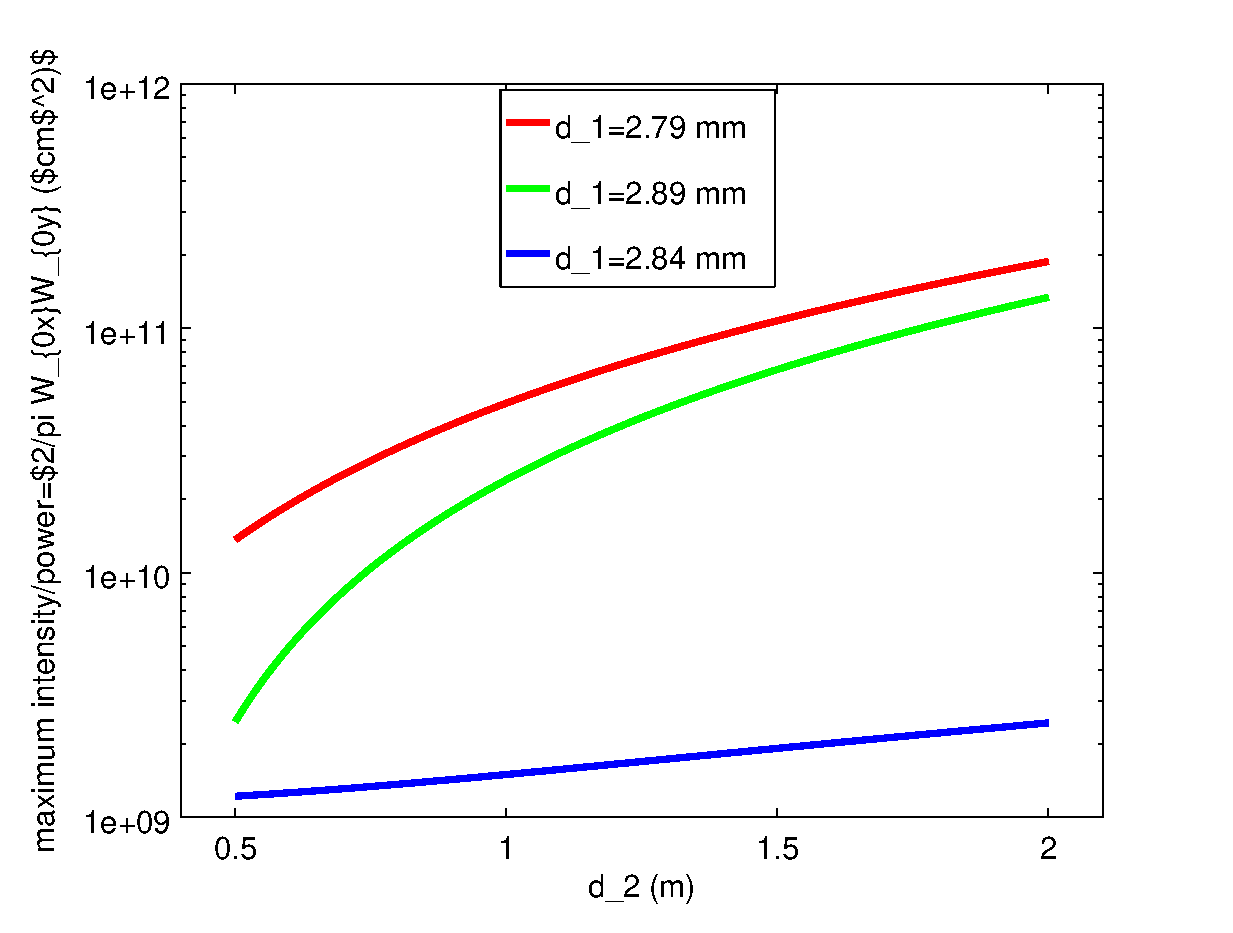
\includegraphics{waists1}}
    %\includegraphics[totalheight=0.3\textheight]{testfigure}
    \caption[]{\label{fig:typicaldata}
    TBA}
\end{figure}

\begin{figure}
    %\centerline{\includegraphics[trim=100pt 100pt 100pt 100pt, clip=true, totalheight=0.5\textheight,angle=90]{testfigure}}
    %\centerline{\includegraphics[totalheight=0.3\textheight]{testfigure}}
    \centerline{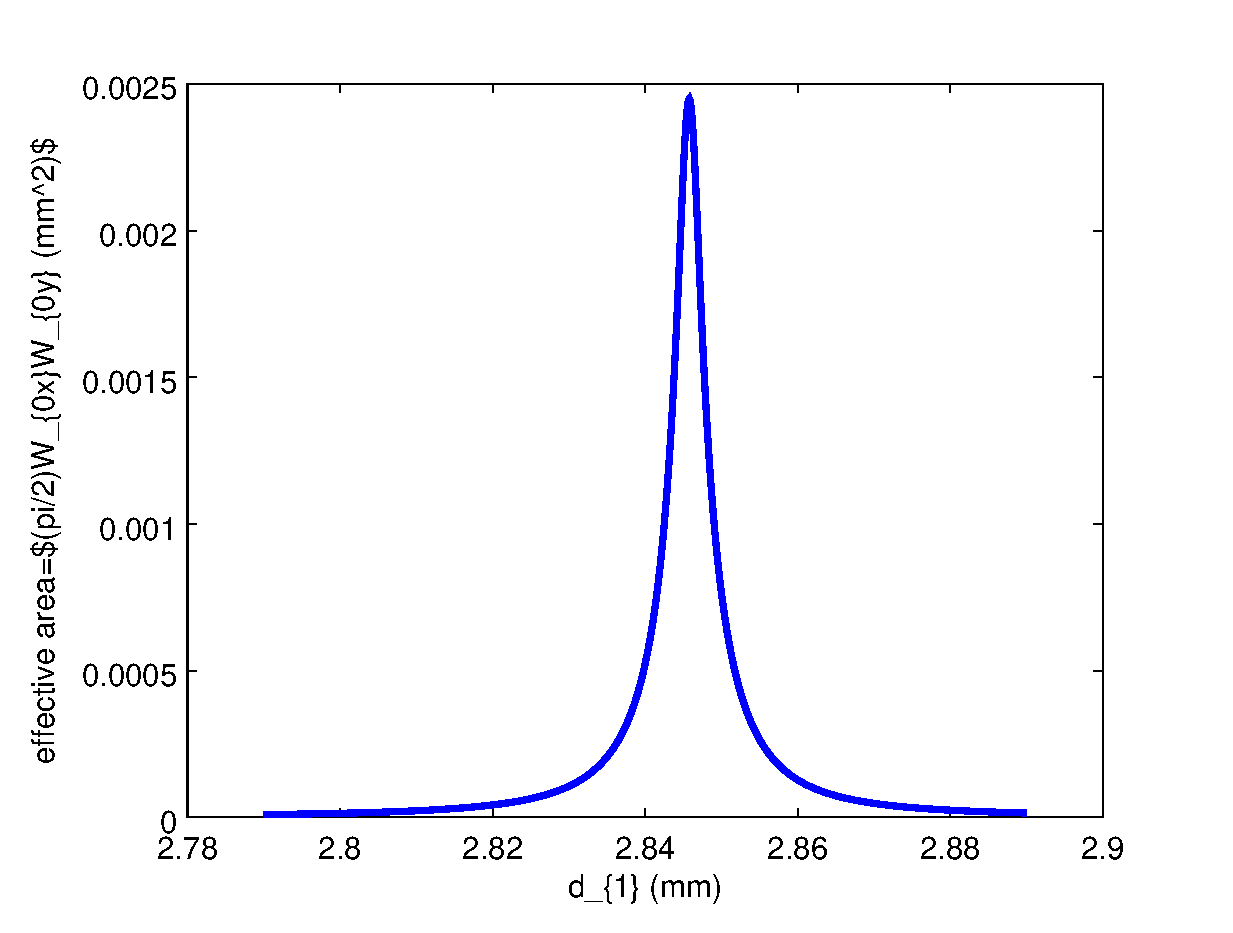
\includegraphics{waists2}}
    %\includegraphics[totalheight=0.3\textheight]{testfigure}
    \caption[]{\label{fig:typicaldata}
    TBD}
\end{figure}




We can talk about that camera. That could be good. %everything is easy once you do it.

 \chapter{Injection Locking}
 %(mode matching, measuring photocurrent from lasers, details of optimizing the isolators, some important caveats about not letting the wrong light couple back into the other laser. 


In order to achieve injection locking, we must couple the first order diffracted light that came out of the AOM into the laser cavities of each of the slave lasers. In this way, we seed the Slave lasers thereby ensure that they will be coupled to the master laser. 
The reason for doing this was to get more power than would have been available from just the shifted beams from the master laser alone. 

\section{Theory of Operation}

%why did this work at all? How did we know how much light would work? 

The laser operates on the principle of stimulated emission of radiation. In a free running laser, the laser's output is determined by the interplay of several factors, including the resonant modes of the laser cavity and the spectral characteristics of the laser gain medium. As light from one mode is amplified, more of the circulating power is in that mode. 
"Mode competition" is the process whereby the power circulating in the laser begins to concentrate in certain, more dominant modes at the expense of others. Since the gain saturation of the diode laser is determined largely by the rate at which electron-hole pairs can be created, it is possible for one mode to dominate the other modes by reaching not only self-saturation, but cross-saturating the gain medium for the other modes. \footnote{saw this on \href{<http://www.rp-photonics.com/gain_saturation.html>}{here}}. 

Therefore, intuitively, the goal of injection locking is to merely couple enough light into a suitable mode of the slave laser so that this mode has a slight advantage over the other modes. 

%did this stuff even work? 
\section{Trying to get the Slaves to have suitable modes}

We selected the slave lasers in a similar way to how we selected the master laser. We used the wavelength-selected diodes \footnote{am I sure?} with the data we took on the Ocean Optics spectrum analyzer. We also adjusted the temperature of the lasers to XXXXXXXXXX.

\section{Matching the mode properly}

For Slave 1, the half-intensity angle was rated to be 9$^\circ$ in the direction parallel to the polarization\footnote{note sure, just has symbols for parallel and perpendicular} and 19$^\circ$ in the perpendicular direction. 

Slave 2 was injection locked. The current produced when coupling the light in from the AOM was 8.2$\mu$A. The current at which it was working was 71.752 mA (27292 counts on the digital controller) and the temperature was found to be 311.309K (59112 counts on the digital controller)\footnote{Lab Notebook section V page 66}. 

Notice that there was something about stray light reflections that we had to be careful of, I think. 

\chapter{Results and Conclusions}

The injection locking was successful and we successfully produced two working beams with an adjustable detuning. 

\section{Spectrum Analyzer}
In this section, we discuss the spectrum analyzer that we built to analyze this system. 

\begin{figure}
%    \centerline{\includegraphics[trim=100pt 100pt 100pt 100pt, clip=true, totalheight=0.5\textheight,angle=90]{spectrumAnalyzer}}
    \centerline{\includegraphics[totalheight=0.3\textheight ]{spectrumAnalyzer}}
    %\includegraphics[totalheight=0.3\textheight]{testfigure}
    \caption[]{\label{fig:spectrumAnalyzer}
    A diagram of the spectrum analyzer. both lasers are coupled to the cavity. One of the mirrors is mounted on piezoelectric devices that allow fine control of its motion. 
}
\end{figure}

The spectrum analyzer is a semiconfocal cavity of length 200 mm. The flat, partially reflective mirror through which light enters the cavity is mounted on a mount that features piezo-electric actuators. At the other end is a curved mirror of focal length 200 mm. Behind this is a photodiode \footnote{the Thorlabs DET XXXXX--probably a DET100A/M or something similar.}.

This is accomplished using a commercially available sweeping piezo control box. 

The length of the optical cavity in the spectrum analyzer can be modulated by sweeping the voltage that we put across the piezoelectric crystals. When the cavity length is such that the coupled light is close to a resonance of the cavity, we expect to see higher signal on the photodiode. 

In order to calculate the Free Spectral Range (FSR) of the cavity, we search for the amount by which the frequency of the coupled light must change as we move from one resonance to the other. 

According to Ref.\ \cite{lasersMilonniEberly}, the equation for the resonant frequencies of the longitudinal modes of our cavity are

\begin{equation} \label{eqModeF}
\nu_{qmn}=\frac{c}{2L}\left[q + \frac{1}{\pi}(m+n+1)\cos^{-1}(\operatorname{sgn}(g_1)\sqrt{g_1 g_2})\right], 
\end{equation}

if we model the resonant modes as Laguerre-Gaussian modes. Here, $L$ is the length of the cavity; $q$ is a nonnegative integer; $m$ and $n$ are integers representing the order of the Hermite polynomials in the solution in the $x$ and $y$ directions. $g_i$ is defined for each mirror and is given by $1-L/R_i$.


From the equation, we see that the hemiconfocal cavity has the special property that many of the resonances align. One of our mirrors is flat, so $g_1=1-L/\infty=1$, while the other's focal length, $f_2$ is equal to the length of the cavity. Recalling that the normal relationship between radius of curvature and focal length is $R_2=2 f_2$, we see that $g_2=1-L/R_2=1-L/(2 f_2)=1-L/(2 L)=1/2$. Thus, 

\begin{equation}
\cos^{-1}(\operatorname{sgn}(g_1)\sqrt{g_1 g_2})=\frac{\pi}{4}.
\end{equation}
Substituting this into Eq.\ \ref{eqModeF}, we see that 

\begin{equation}\label{freq_semiconfocal}
\nu_{qmn}=\frac{c}{2L}\left[q + \frac{1}{4}(m+n+1)\right], 
\end{equation}

Since $m$,$n$ and $q$ are all integers, we see that the resonant modes will be integer multiples of $c/(8L)$. Eq.\ \ref{freq_semiconfocal} also demonstrates one of the nicest features about semi-confocal cavities, which is that different transverse modes of the electric and magnetic have the same resonant frequency. Thus, rather than having to couple carefully to the TEM$_{00}$ mode, we can allow the light to couple to any transverse mode of the cavity. If we assume that we are coupled to many cavity modes, we can safely assume that adjacent resonant frequency peaks are separated by $c/8L$, which is the Free Spectral Range of the cavity. 

Interestingly, the hemiconfocal configuration has an advantage over \footnote{I am going out on a limb here...} the confocal configuration that is illustrated by this equation. In the confocal configuration, both mirrors are identical and are placed so that their focal points coincide. This means that $L=R_1/2=R_2/2$ and thus $g_1=1-L/R_1=g_2=1-L/(2L-R_2)$. Therefore, $\sqrt{g_1g_2}=0$, making the free spectral range of the cavity $c/4L$. However, note that if $L$ changes, then the sign of $g_1$ changes, leading to a kink in the frequency response. With a hemiconfocal cavity, there is no such discontinuity. This makes the expansion in the next section slightly easier. 

Note that we are note actually scanning the frequency of the laser. Rather, it is the length of the cavity that scans. Note, however, that both confocal and hemiconfocal cavities remain good, stable cavities as their lengths are scanned since the condition for cavity stability is that $0\leq g_1 g_2 \leq 1$. 

The piezoelectric mount (Thorlabs KC1-PZ) is rated to accept a maximum voltage of 150 V and provide a maximum of $\pm4\mu$m of linear travel. Thus, since our sweep voltage is only about 75 V, we expect that our cavity should be sweeping ~2$\mu$m. If the wavelength of the light is 408 nm, we expect that for each 2$\mu$m of displacement, we should see about $8*2\mu$m$/408nm \approx 40$ resonant peaks. This is a good order of magnitude estimate for the most peaks we can see. Therefore, we can say that the change in cavity length, $\Delta L< 2\mu$m.

Now, if we take Eq.\ \ref{eqModeF} and make the following substitutions:
\begin{align}
g_1&\rightarrow1 \text{ (since $R_1=\infty$)} \\
g_2&\rightarrow 1-L/(2L)\\
L&\rightarrow L(1-\epsilon)\\
\end{align},

we get 

\begin{equation} \label{eqModeF_ready_for_expansion}
\nu_{qmn}=\frac{c}{2L(1+\epsilon)}\left(q+\frac{m+n+1}{\pi}\arccos(\sqrt{1-L(1-\epsilon)/(2L)})\right)
\end{equation}.

Note that we have used $R_2=2L$ and not $R_2=2L(1+\epsilon)$ since the radius of the mirror does not change as we sweep the cavity. 

We now make a Taylor expansion of Eq.\ \ref{eqModeF_ready_for_expansion} using Mathematica, we get 
\begin{align*}
\nu_{qmn}=\frac{c}{8L}\biggl((4q+m+n+1) +\\
 \left(-4q-m-n-1+\frac{2}{\pi}(1+m+n)\right)\epsilon+\\
 \left(4q+m+n+1+\frac{2}{\pi}(1+m+n))\right)\epsilon^2\\
 \left(-4q-m-n-1+\frac{7}{3\pi}(1+m+n)\right)\epsilon^3\\
 \left(4q+m+n+1-\frac{7}{3\pi}(1+m+n)\right)\epsilon^4\\
\biggr)
\end{align*}

The coefficient for the first order expansion in terms of $\epsilon$ contains integers $m$,$n$ and $q$ as we expect. 
However, it might seem unnerving at first that it also contains coefficents like $2/\pi$ that are of order unity! The reason this is ok is that $q>>m,n$. We know this is the case for two reasons: First, the Laguerre Gaussian modes are derived using the paraxial wave approximation. The paraxial wave equation assumes solutions of the form
\begin{equation}
\vec{E}(\vec{r},t)\approx \mathcal{E}(\vec{r})\exp[i(kz-\omega t)]
\end{equation}
and it relies on the fact that 
\begin{equation}
\left|2k\frac{\partial \mathcal{E}(\vec{r})}{\partial z}\right|\gg\left|\frac{\partial^2\mathcal{E}(\vec{r})}{\partial z^2}\right|
\end{equation}
Since the derivatives of $E(\vec{r})$ depend on $m$th and $n$th order Hermite polynomials, we see that our equations only hold up when $m$ and $n$ are reasonably small. 

This can also be easily seen since the cavity length is 20cm, while the cavity mirrors are about 1 cm across and the laser modes in the cavity can be seen to be less than 5 mm in diameter. One may imagine intuitively that the number of nodes along a long dimension (represented roughly by $q$) is going to be large compared to the number of nodes created by light at the same frequency along a much smaller distance. 

\footnote{Now, I'm not sure whether it's the case that our approximation breaks down and that's why the $m$ and $n$ have to be small. It seems intuitive to me that you can get a lot more oscillations at a given frequency in a 20cm space than you can in a 1 cm space, but I'm not sure if that's the right intuition.\cite{lasersMilonniEberly} eq. 7.8.17 might have some decent insight. All the modes have the same $R(z)$ and $w(z)$, but I think there's more power out of the bucket as they say.  }

This might be OK. If, for example, we assume the argument in the radical ($1-L(1+\epsilon)/(2L)\approx 1/2$ for all values of $\epsilon$, then we get this expansion: 

\begin{align}
\nu_{qmn}=\frac{c}{8L}
\end{align}



If we assume that we are coupled to many different modes, we can assume that the nearest peaks on our spectrum analyzer represent a change of 

It would, of course, be possible, to suppress some of the modes by coupling our beam in carefully, 

A simple ray-tracing argument can also be used. 
\begin{figure}
\centerline{\includegraphics[height=3cm]{spectrum_analyzer_path.png}}
\caption{Illustration of the optical path that makes a complete trip around the semiconfocal cavity. Note that the ray traverses the entire length of the path four times before doubling back on itself. It traverses the path 8 times before ending up in the same place again. This diagram similar to one found on page 277 of Ref.\ \cite{lasersMilonniEberly}}
\end{figure}

In order for the cavity to be resonant with our light, the full optical path of the light must be an integer number of wavelengths. The resonance condition is 
\begin{equation}
n \lambda = d
\end{equation}
where $n$ is an integer, $\lambda$ is the wavelength and $n$ is the length of the optical path in the cavity. 
For a semiconfocal cavity, we see that a ray parallel to the optical axis would have to traverse the cavity length 8 times before finally getting back to its starting point. 

This argument may prove that any mode of the cavity will find resonances spaced by $c/8L$.

%Probably there is some way in which we can talk about a Gaussian mode that makes the Gouy phase shift somehow explainable in terms of two (or more!) crossing rays of propagation. 



Perhaps the resonant length of the other modes is not because they travel farther off-axis. It's perhaps related to some other issue that arises when we move the focal points.




First, we examine the output of the spectrum analyzer when we couple both Slave lasers into it. 
The two peaks clearly correspond to the two slave lasers. We can see that there is a lot of power \footnote{honestly, I'm not sure that all the power coming out was in those modes. It was a little bit flaky}
We can clearly identify which peak corresponds to which Slave laser by blocking one of the slaves. 

\section{}

Next, we attempt an experiment whereby we adjust the driving frequency. We should be able to see the peaks shifting by an amount corresponding to the change in the frequency. This will provide strong evidence that the two slaves are, in fact, injection locked to the modulated beams coming out of the AOM. 

This test has the further benefit of confirming that we have calculated the free spectral range of the cavity in the spectrum analyzer correctly. 

%where is the energy going? I think it goes from reflecting to transmitting

 
\begin{figure}
    %\centerline{\includegraphics[trim=100pt 100pt 100pt 100pt, clip=true, totalheight=0.5\textheight,angle=90]{testfigure}}
    %\centerline{\includegraphics[totalheight=0.3\textheight]{testfigure}}
    \centerline{\includegraphics{sampleOffsetData}}
    %\includegraphics[totalheight=0.3\textheight]{testfigure}
    \caption[]{\label{fig:typicaldata}
    We changed the detuning on our frequency generator in something like 10 MHz increments. These are some of the data that we have that show the spacing between our peaks changing in a predictable way.}
\end{figure}
\begin{figure}
\centerline{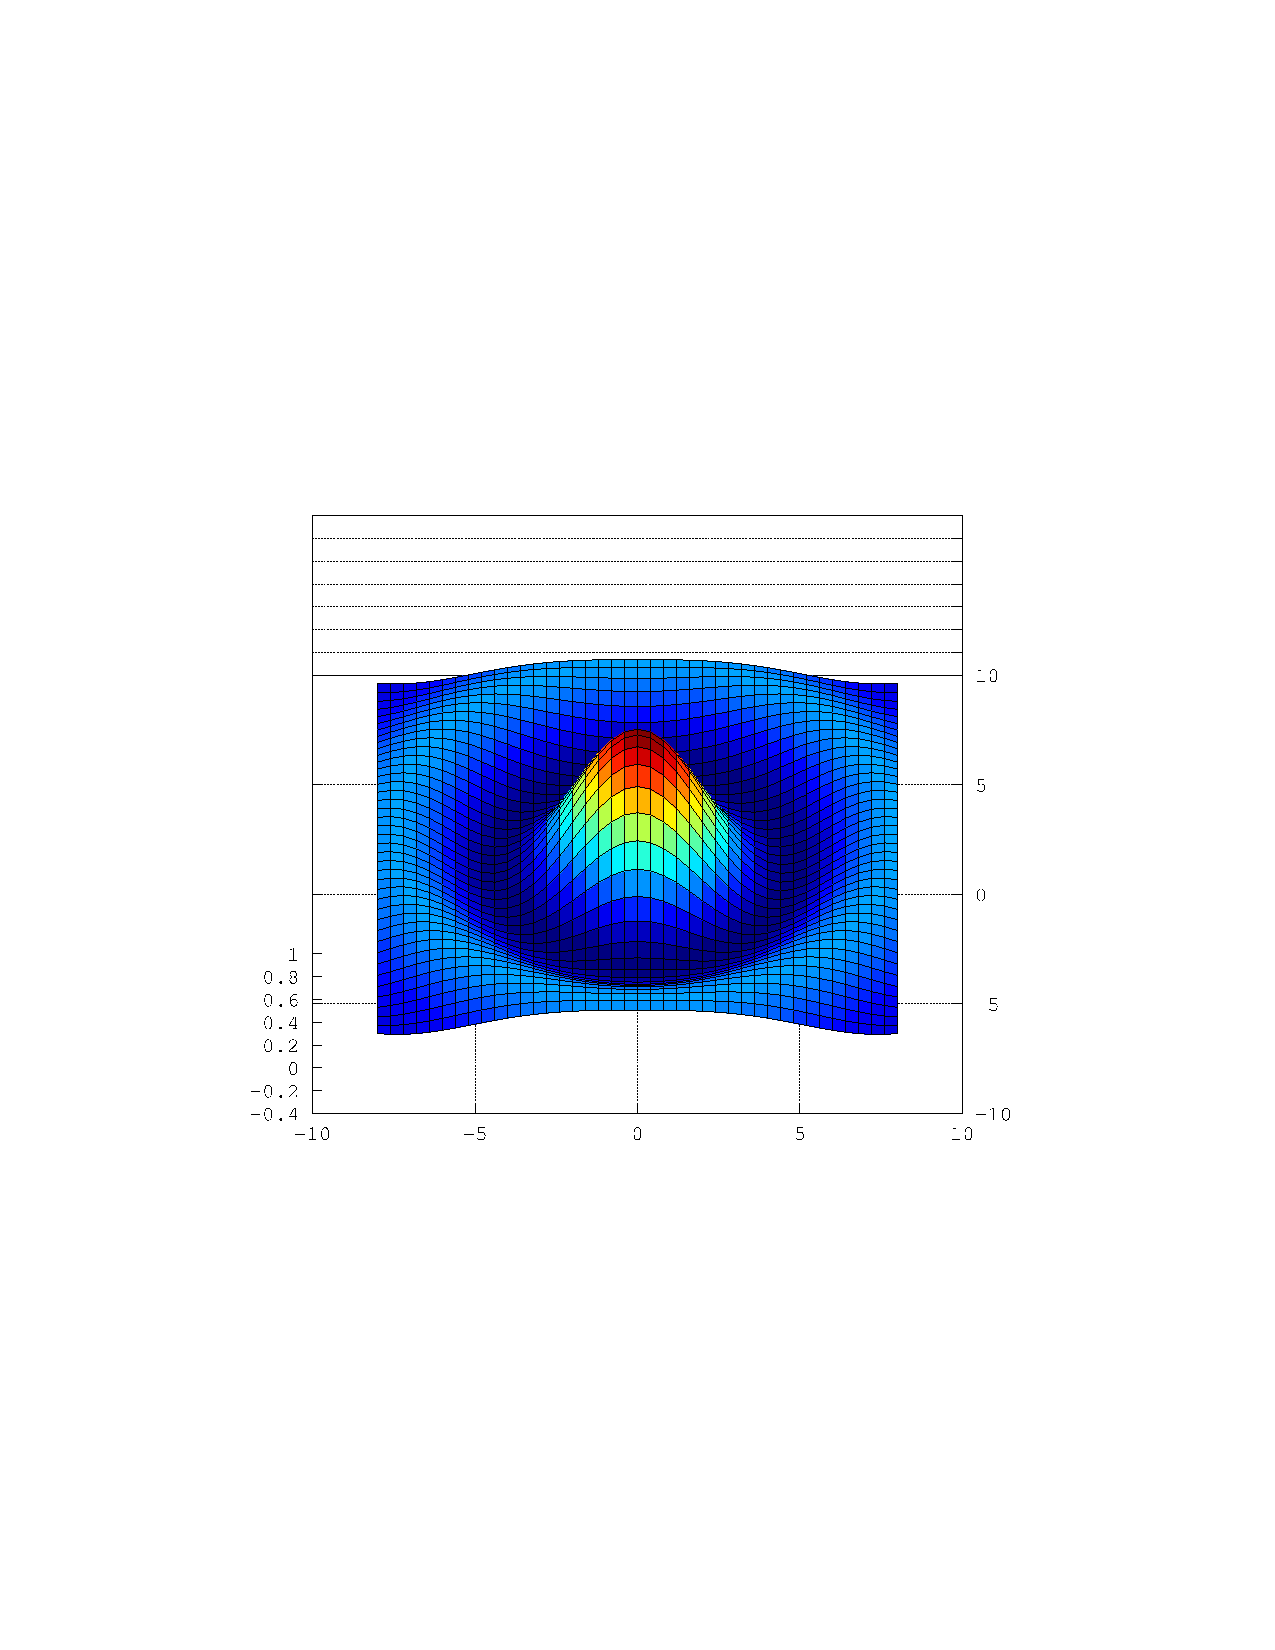
\includegraphics{thisone}}
\end{figure}

\begin{figure}
\centerline{\includegraphics{all_splittingData}}
\caption[]{\label{fig:alldata} 
This is the complete set of data from which the previous graphic was culled. Some of it is clipped uglily. The peaks are on top of each other, but it may have drifted to a higher power between when I set it up and when I took the data. I'm not sure why this looks so much worse than the data I normally take.}
\end{figure}

Also, I have data that I can analyze to examine the feasibility of a Chu lock. I recorded 999 traces that showed the output of the spectrum analyzer, the current and the voltage. I recorded these over several hours, during which the laser drifted into and out of good, single mode operation. In principle, this data could be analyzed. 

We have shown that we can change the oscillator frequency and thereby change the detuning. There is a limit to the extent that we can do this. (Notice in Fig.\ \ref{fig:alldata} that the peaks get small as we continue to detune.) However, this is due to geometry. When I realigned using the method of measuring the photocurrent coming out of the slave lasers, I found that I was able to get the thing to work over an entirely different range of oscillator frequencies. 



\appendix
\bibliographystyle{phBYU}
\bibliography{mybib}
 
\chapter{Measuring Beam Waist}
\label{BeamWaistAppendix}

Sometimes it's important to measure the waist of one's laser beam. This explains the exact method we use. 
  
The profile for the intensity of the beam is given by

\begin{equation} \label{electricFieldExplicitForm}
I(r,z)=I_0\left(\frac{w_0}{w(z)}\right)^2 \exp \left(\frac{-2 r^2}{w^2(z)}\right)
\end{equation}

Extrapolating this to when there are two different waists in different directions, we get: 

\begin{equation}
I(r,z)= ({\rm constants})\exp \left(-2\frac{x^2}{w_x^2(z)}-2\frac{y^2}{w_y^2(z)}\right) . 
\end{equation}

Now, total power ($P$) can be obtained by integrating the the intensity: 

\begin{align}
P&=\int_{-\infty}^{\infty}\int_{-\infty}^{\infty} ({\rm constants}) \exp \left(-2\frac{x^2}{w_x^2(z)}-2\frac{y^2}{w_y^2(z)}\right) dx dy\\
P&=\frac{\pi}{2} ({\rm constants}) w_x(z) w_y(z)
\end{align}

Now, we figure out that those constants will be

\begin{equation}
({\rm constants})=\frac{2 P}{\pi w_x(z) w_y(z)}.
\end{equation}

The ``constants'' term represents the maximum intensity that occurs within the beam (i.e. when $x=y=z=0$, or in other words, at the center of the narrowest part of the beam.)

Now, to take measurements with a knife, we block some fraction of the beam by mounting the knife on a translation stage. We then look at the amount of power from the beam hitting a photo diode that is placed downstream from the knife. If, for example, the knife is mounted vertically, the measurements on the photo diode correspond to the total power in the beam from $x=-\infty$ to $x_0$ where $x_0$ is the location of the knife. Thus, if we plot this power as a function of the spatial position of the knife, we expect that the result should be 

\begin{align}
P(x_0)&=\int_{\infty}^{\infty}\int_{-\infty}^{x_0} \frac{2 P}{\pi w_x(z) w_y(z)}\exp \left(-2\frac{x^2}{w_x^2(z)}-2\frac{y^2}{w_y^2(z)}\right) dx dy\\
P(x_0)&=\frac{P}{2} \left(\erf \frac{\sqrt{2} x}{W_x}+1 \right)
\end{align}

So, now we have a function that we can fit. The code in masterFILEhoriz14Nov.m calculates the approximate beam waist based on a series of knife cuts. First, one loads the intensity (in arbitrary units) and the position (in the units that the waist will ultimately be given in) into a number of arrays named x1, x2, .. . etc. The user types the position of the knife along the waist (show picture) into the vector called positions. 

The function d4sigma attempts to calculate the second moment width using just the raw data. This is notoriously inaccurate and also it is probably misnamed because it probably just calculates something that is different from the standard D4$\sigma$ by some factor of 2 or something. Also, we don't use this. 

Ultimately, the program does a best fit approximation to a Gaussian for each beam profile. The function we fit to is contained in the file beamWaistCalculator, which takes as its arguments the raw position data and the raw intensity data. This function is 

\begin{equation}
f(x)=a_1 \erf \left(\frac{x-a_3}{a_2}\right)+a_4.
\end{equation}

beamWaistCalculator thus returns a vector containing $(a_1 a_2 a_3 a_4)$. Thus, to get the beam waist, we will take $a_2$ and multiply by $\sqrt{2}$. 

According to Siegman \cite{SiegmanBeamQuality}, the second moment width always propagates according to this equation: 

\begin{equation}
W_x^2(z)=W_{0x}^2 + M_x^4 \left( \frac{\lambda}{\pi W_{0x}}\right)^2 (z-z_{0x})^2. 
\end{equation}
Of course, for a Gaussian beam, we recognize that allowing $M_x^2\rightarrow 1$ gives us the equation for how the waist changes as it propagates. 

This function then tries to fit to this:
\begin{equation}
W_x=a_1 \sqrt{1+\left(\frac{(x-a_2) \lambda}{\pi a_1^2}\right)^2}
\end{equation}
and this:
\begin{equation}
W_x=a_1 \sqrt{1+(1+a_3^2) \left(\frac{(x-a_2) \lambda}{\pi a_1^2}\right)^2}. 
\end{equation}
The first case we are forcing $M^2$ to be one. This gives us a worst-case scenario. A few test cases convinced us that if $M^2$ is higher than we think it is, we have a less-tightly focused center. Thus, for the purposes of not putting too much power into the AOM, we go with the fit to the first equation. 

In principle, we should be able to fit the calculated second moment widths to the equations above, but they don't work overly well. Thus, we usually use the second moment width of the Gaussian we fit it to. 

Using this method, we have determined the waist to be 


\section{Using the camera}
We initially wanted to measure the $M^2$ of our beam. The measurements are hard to do accurately. We tried to use the camera and got results that were not entirely usable.

\subsection{Investigation of feasibility of using the camera}

The camera seems like an appealing device to use to measure beam parameters since it can take large amounts of 2D data quickly.

%insert plot of pixel count vs whatever? eh, maybe.

To investigate the camera's feasibility, we wanted to verify that the camera was (a) linear and (b) that each pixel reading was independent of the rest of the image. To this end, we took several images of the same beam, which we attenuated using the polarizing beam cube/wave plates adjustable attenuator setup described in Appendix\,\ref{twoWaveplateTrick}. We took 20 measurements. Each time we measured the total intensity of the beam using a photo diode and we took a corresponding image of the beam

\begin{figure}
\centerline{
\includegraphics[width=0.95\textwidth]{cameraimage}
}
\caption[Sample camera images]{Three images taken using the camera. Each was the same laser beam with the attenuation adjusted using our wave plate and polarizer setup. The total power was measured using a photo diode and the relative total power is shown in the lower right corner of each image. By comparing the pixel values of similar spots within the image, we were able to bootstrap some calibration parameters for the camera.}
\end{figure}

Our idea was that, if the camera is linear and the pixels act independently, the following statements should be true: 
\begin{itemize}
\item The ratio of the reading on any pixel to the reading on the same pixel in a different image should be equal to the ratio of the total power of the two beams used in the two readings as measured by the photo diode. 
\item Any two pixels reporting the same number of counts are experiencing the same radiance.
\end{itemize}

Thus, for example, if we see that the pixel located at $(214,442)$ has a pixel count of 127 in image 15, on which we measured the intensity to be proportional to 85.350, then we assume that we can compare it directly to a pixel located at the same location $(214,442)$ on image 20 (which had an intensity proportional to 119.70). If the reading from the $(214,442)$ pixel on image 20 was 155.46, we assume that a pixel count of 155.46 corresponds to $119.70/85.350=1.4025$ times as much intensity as a pixel count of 127. Additionally, we assume that any pixel we find in any of the images that reports a reading of 155.45 will have the same intensity as any other. 

We went through the 20 images like this: We selected some reference pixel. We then added that pixel to a master list. We then found the corresponding pixels in the other images whose position on the grid match that of the reference pixel. They were then added to the master list, making note of their position, the reading on the pixel (count) and the assumed ratio between the amount of light hitting that pixel and the amount of light hitting reference pixel as inferred based on the readings from the photo diode.

Then, we select a random pixel from the master list and look for other pixels that have the same number of counts within any of the images. If a pixel has the same reading (number of counts) as the randomly selected pixel in the master list, it is added to the master list. Since this new pixel has the same counts as the randomly selected pixel, we assume that the pixels have the same radiance relative to the reference pixel. Once the new pixel is added to the master list, we find the corresponding pixels from the other images and add them to our list. We assume that the true irradiance at these pixels is proportional to the irradiance of pixel we just added. 

In this way, we create a very long list of pixels, their counts and what we have inferred about the incident illumination of each pixel by comparing it to (a) other pixels that read the same value and (b) pixels in other images of different intensities. Note that the pixels in the list are not unique. Pixels can appear multiple times in the list.

If we plot the expected pixel count (as calculated by taking the reading on the main reference pixel and multiplying it by the relative radiance factors that we've been tracking) vs the actual pixel count, we get the plot in Fig.\,\ref{cameraPixelFit}, which seems to validate the assumption of pixel independence.

However, as one can see, the camera actually has a minimum threshold below which it does not report light very well. Because the camera throws away information and has a minimum intensity threshold to register, we throw out any $M_{i j}=0$. This way our function doesn't get penalized for showing a non-zero intensity for pixels that read out zero. The number of $M_{i j}=0$ obviously doesn't change as we try different iterations of $f(M_{ij})$, so there's no way to game our little metric to make it not work.
%We did a standard fit to a 4th order polynomial and got a reasonable function to correct for the pixel values. We were a little worried about bias in the selection of pixels and things like that. We wasted some time trying to figure out how to do this better. 

We performed a curve fit to model our pixels response. In order to do this, we had to devise a cost function that produces some figure of merit to tell us whether our test function is succeeding at making all of the pixels have the right ratio. The way it works is this: Suppose that $M_{i j}$ is a big list of our pixels. $j$ runs from 1 to 20, corresponding to the 20 different images. $i$ represents all the pixels in our image\footnote{Thus, if we are analyzing 8x8 bins, we should have 480/8*640/8=4800 pixels and i will range between 1 to 4800}. Let $f(p)$ be the proposed function that takes as its argument the count on a given pixel and gives as its output something that scales with the actual intensity of the light. The figure of merit that we can use to optimize $f(p)$ is calculated as follows: 

\begin{equation}\label{fom}
{\rm Figure\:of\:merit}=\sum_{ M_{i j}\neq 0}\left(\frac{f(M_{i j})/P_j}{{\rm average\,of\,all\,nonzero\,} f(M_{i j})/P_j {\rm \,for\,the\,ith\,pixels}}-1\right)^2
\end{equation}

where $P_j$ is the power of the j th image.

In words, Eq.\,\ref{fom} can be described as follows: First, act on the pixels with the proposed function. Then, scale them according to the intensity ratios (i.e. the i th pixel in image 1 gets divided by $P_1$ while the i th pixel in image 3 gets divided by $P_3$). Then, see by what fraction the intensity of that pixel differs from the average of the intensities calculated using data from the pixels corresponding to that one. If the function really were to find the ratio perfectly, then $f(M_{ij})/P_j$ should be exactly the same for the i th pixel from each of the j images. 


We used this function to calculate what correction function to use. We did a couple of them and found great agreement with the inversion of the previous function--thus suggesting that our previous method was acceptable. 


\begin{figure}
\centerline{
\includegraphics[width=0.95\textwidth]{cameraPixelFit}
}
\caption[Camera linearity and offset]{On the x axis is the inferred pixel reading based on our assumptions about the ratios of pixel readings. On the y axis, we can see the actual readings of the pixels. This illustrates clearly the threshold issue of the camera. In the top, left side of the plot, there is clearly a region where our inferred readings should be nonzero, but the actual readings on the camera remain at zero.\label{cameraPixelFit}}
\end{figure}

In the end, the camera offset and nonlinearity made it unsuitable for sensitive measurements of the second moment width of the beam. However they did provide a reasonable sanity check on our methods.
%\end{document}

\include{AppendixTryingtoFigureouttheChuLock}
\include{AppendixFreeSpectralRangeDerivation}
\chapter{Optimizing Motion of External Cavity Grating}\label{GratingRatioAppendix}
In order to narrow the line width of the master laser and make it more tunable and stable, we have mounted a diffraction grating in a Littrow configuration. The gratings are mounted on piezoelectric actuators that can be automatically moved in unison by our control circuitry. 

However, in order for this to work, it is important to verify that the piezos can be scanned in such a way that the resonances of the external cavity track smoothly. In order to accomplish this, one must find a ratio that relates the relative rates at which each piezoelectric actuator is scanned. As explained in Section \ref{ensuringAbilityToFineTune}, the length of the cavity and the angle of the grating must change in such a way that the wavelength featured by each changes at the same rate for small displacements. 

For many configurations, this is not very tricky. However, at one point we discovered that for certain geometries, the appropriate ratio might be negative. To this end, we created the following Mathematica notebook to model the motion of the grating and help us to ensure that our electronics are capable of moving the actuators properly. 

In practice, the results of this calculation would typically be used only as a starting point. In order to really get the laser working well, the experimenter usually adjusts the ratio iteratively in order to maximize the range over which the frequency of the laser can be scanned without mode hopping. 

\includepdf[pages={1-10}]{grating_motion}



\chapter{Spectrum Analyzer}
\label{Spectrum Analyzer}





In this Appendix, we discuss the Fabry-Perot spectrum analyzer that we built to analyze this system. 


\section{Spectrum analyzer design}
One of the mirrors is mounted on a Thorlabs kinematic piezo mount and attached to a piezo driver designed specifically for spectrum analyzers.

The cavity is designed to be nearly semiconfocal.%\footnote{I used to think that this was because the transverse modes of a semiconfocal cavity overlap. However, it seems that a concentric cavity would be more likely to have this property. Oh wait. I get it. The semiconfocal cavity has all its transverse modes very small.} 
This is because a semiconfocal configuration is one of several in which many modes are degenerate, such that liht coupling to different transverse modes come into resonnance at the same frequency. This makes it possible to get very sharp, clear features without having to carefully couple to one specific transverse mode of the cavity. 

%\footnote{How do I know whether I'm semiconfocal for all practical purposes? I mean, somehow lower finesse should make me less sensitive to small variations in the cavity length. Furthermore, are there models where the errors never really go away? You know? I guess I mean where it doesn't just become part of the noise. I suppose chaos is one example of this--where arbitrarily high precision is needed to predict even the macroscopic behavior of the system. Is any aspect of this system chaotic?}

\section{Free spectral range basics}
The Free Spectral Range (FSR) of the cavity is defined as the difference in frequency between adjacent resonant longitudinal modes of the cavity. It always works out to be $c/2L$. 
It is easy to condsider the example of a one-dimensional cavity with just one transverse mode. If we suppose that we have some wavelength $\lambda$ that is resonant with our cavity, then the resonant condition would be that 
\begin{equation}
m\lambda=2L
\end{equation}
where $m$ is an integer and $L$ is the cavity length (center to center distance between the surfaces of the cavity mirrors). In other words, we require that for a mode to be resonant with our cavity, the total optical path length of a trip around the cavity (in this case, twice the cavity length) must be divisible by the wavelength of the light. We can find other wavelengths of light that satisfy the resonance condition. So, for example, we might be able to find some wavelength $\lambda'$ that satisifes
\begin{equation}
(m+1)\lambda'=2L
\end{equation}

The free spectral range would just be the difference in frequencies corresponding to $\lambda$ and $\lambda'$. Using $\lambda = c/f$, we see that 
\begin{equation}
m\lambda= 2L \rightarrow \frac{mc}{f}=2L
\end{equation}
which we can solve for $f$ to find 
\begin{align}
f-f'&= \frac{(m+1)c}{2L}-\frac{m c}{2L}\\
&= \frac{c}{2L}
\end{align}

where $f'$ and $f'$ are the frequencies associated with $\lambda$ and $\lambda'$ respectively. 

\section{Free spectral range for real cavities}
In general, there will be more than one transverse mode. The free spectral range remains $c/2L$. However, between any two peaks corresponding to one transverse mode, there will be other resonant peaks corresponding to other transverse modes. Thus, there will be resonances of our cavity spaced closer than the free spectral range. One could, in principle, couple to just a single transverse mode by carefully coupling the beam to the cavity.

However, in our system this is not necessary. We use a semiconfocal (hemiconfocal), which has the convenient property that the various transverse modes line up in such a way that they fall into four distinct, evenly-spaced groups. Therefore, if we couple to many transverse modes of the cavity, we expect that our effective free spectral range will be $c/8L$.

%\footnote{Look, I was very confused about the factor of 8 for a long time. I now realize that I was simply misinterpreting the normal ray transfer diagram I had in my mind of a confocal cavity. Also, I was not very clear on why semiconfocal was the one where different transverse modes overlap. Since I've found the answers, I figured I might as well put them here.} 
\section{Derivation of free spectral range for hemiconfocal cavities}
\begin{figure}
\centerline{\includegraphics[height=3cm]{spectrum_analyzer_path.png}}
\caption[Spectrum analyzer ray path illustration]{\label{completePath}Illustration of the optical path that makes a complete trip around the semiconfocal cavity. Note that the ray traverses the entire length of the path four times before doubling back on itself. It traverses the path 8 times before ending up in the same place again. This diagram similar to one found on page 277 of Ref.\ \cite{lasersMilonniEberly}. Here, we assume that the ray travels nearly parallel to the central axis of the cavity so that the length of each leg is well-approximated by the length of the cavity, $L$.}
\end{figure}

This can be illustrated with a simple ray-tracing argument. 
In order for the cavity to be resonant with our light, the full optical path of the light must be an integer number of wavelengths. The resonance condition is 
\begin{equation}
n \lambda = d
\end{equation}
where $n$ is an integer, $\lambda$ is the wavelength and $d$ is the length of the optical path in the cavity. 
For a semiconfocal cavity, we can convince ourselves visually (see Fig.\,\ref{completePath}) that a ray parallel to the optical axis would traverse the entire length of the cavity 8 times before finally getting back to its starting point. Thus, we expect that $d\approx 8L$.
We therefore expect that modes in the cavity will have resonant frequencies spaced by $c/8L$. 


\section{Using the paraxial wave equation}

A more rigorous treatment of this can be done by solving the paraxial wave equation. This model will also allow us to model the exact behavior of our real life cavity (note that in the real cavity, we look at just a handful of wavelengths but we scan the cavity length).

\subsection{Review of paraxial wave equation}

We first examine the equation describing the electric field for different modes of the cavity. This can be derived directly from Maxwell's equations using the paraxial approximation (see, e.g., Refs.\ \cite{lasersMilonniEberly} and \cite{bergeson_amo_notes} for a complete discussion of this). The argument in brief is basically this: 

\begin{itemize}
\item Assume that the three-dimensional electric field can be represented by a scalar quantity $E(\mathbf{r},t)$
\item Recall Maxwell's equations with no nearby charges or currents give rise to the wave equation $\nabla^2E(\mathbf{r},t)-\frac{1}{c^2} \frac{\partial^2}{\partial t^2} E(\mathbf{r,t})=0$
\item Assume solution takes the form $E(\mathbf{r},t) = \mathcal{E}_0(\mathbf{r}) \exp(i(kz-\omega t))$ and plug this into the wave equation above. 
\item Make the paraxial approximation: Assume that $\lambda \left|\frac{\partial \mathcal{E}}{\partial z} \right| \ll |\mathcal{E}_0|$ and $\lambda \left| \frac{\partial^2\mathcal{E}_0}{\partial z^2}\right| \ll \left| \frac{\partial \mathcal{E}_0}{\partial z}\right|$. In other words, we assume that the wiggling
%\footnote{I think this word is so funny, but I might change it} 
is mostly happening along the $z$ direction. 
\end{itemize}

This leads to the paraxial wave equation: 
\begin{equation}
\left(\frac{\partial^2}{\partial x^2}+\frac{\partial^2}{\partial y^2}+2ik\frac{\partial}{\partial z}\right) \mathcal{E}_0(\mathbf{r})=0 \label{final_paraxial_wave_eqn}
\end{equation}

The solutions to Eq.\ \ref{final_paraxial_wave_eqn} can be shown to be of the form:

\begin{align} \label{solutionToParaxial}
\mathcal{E}_{mn}(x,y,z)=&\frac{Aw_o}{w(z)}H_m\left[\sqrt{2}\frac{x}{w(z)}\right]H_n\left[\sqrt{2}\frac{x}{w(z)}\right] \\
&\times \exp(i(kz-(m+n+1)\tan^{-1}(z/z_0)\\
&\times \exp(ik(x^2+y^2)/2R(z)) \exp(-(x^2+y^2)/w^2(z))
\end{align}

Here, $\mathcal{E}$ is the magnitude of the electric field. $H_m$ and $H_n$ are the (physicists') Hermite polynomials of degree $m$ and $n$\footnote{If we ever were to need a real solution to the equation, we could find one by simply taking: $\mathcal{E}+\mathcal{E}*$.}. $R(z)$,$z_0$,$w_z$ and $w_0$ are defined in the same way that they are for a Gaussian mode:

\begin{align}
w(z)&=w_0 \sqrt{1+\frac{z^2}{z_0^2}} \\
R(z)&=z+\frac{z_0^2}{z}\\
z_0&=\frac{\pi w_0^2}{\lambda }
\end{align}

%\footnote{I'm not sure why this works when we neglect polarization. It seems like you might get accidentally a factor of 2 or something extra based on the polarization diagram that Milloni and Eberly have on page 305. Perhaps there is another factor of 2 somewhere else? }

\subsection{Frequencies of resonant modes}
Now, the propagation of the solution to the paraxial wave equation from \ref{solutionToParaxial} can be calculated using Eq.\ \ref{ABCDlawforGaussianBeams}. The resonant condition is that after propagating across the cavity an arbitrary number of times, a beam must be the same\cite{lasersMilonniEberly}.
Alternatively, we may demand simply that $R(z)$ (which we interpret as the radius of the wavefronts) at the location of each of the mirrors match the radius of the mirror. This condition on $R$ is sufficient to guarantee that the cavity mode the light is traversing is stable. In order to have a resonant mode (as opposed to a mode that is merely stable), the light must also accumulate a phase change that is some integer multiple of $2\pi$ after traversing the cavity a finite number of times.
%and that the the cavity length be an integer multiple of wavelength. 

Following this reasoning, Ref.\ \cite{lasersMilonniEberly} gives the following equation for the resonant frequencies of the longitudinal modes of our cavity:

\begin{equation} \label{eqModeF}
\nu_{qmn}=\frac{c}{2L}\left[q + \frac{1}{\pi}(m+n+1)\cos^{-1}(\operatorname{sgn}(g_1)\sqrt{g_1 g_2})\right], 
\end{equation}

%if we model the resonant modes as Laguerre-Gaussian modes. 
Here, $L$ is the length of the cavity; $q$ is a nonnegative integer; $m$ and $n$ are integers representing the order of the Hermite polynomials in the solution in the $x$ and $y$ directions. $g_i$ is defined for each mirror and is given by $1-L/R_i$. The term involving $g_1$ and $g_2$ will depend strictly on our cavity geometry\footnote{It may seem strange that Eq.\,\ref{eqModeF} depends on the sign of $g_1$ and not $g_2$. However, this equation is valid only for stable cavities and the condition for a stable cavity is that $0\leq g_1 g_2 \leq 1$. Thus, we can assume that $g_1$ and $g_2$ have the same sign.}.

From Eq.\,\ref{eqModeF}, we see that the hemiconfocal cavity has the special property that many of the resonances align. One of our mirrors is flat, so $g_1=1-L/\infty=1$, while the other's focal length, $f_2$ is equal to the length of the cavity. Recalling that the normal relationship between radius of curvature and focal length is $R_2=2 f_2$, we see that $g_2=1-L/R_2=1-L/(2 f_2)=1-L/(2 L)=1/2$. Thus, 

\begin{equation}
\cos^{-1}(\operatorname{sgn}(g_1)\sqrt{g_1 g_2})=\frac{\pi}{4}.
\end{equation}
Substituting this into Eq.\ \ref{eqModeF}, we see that 

\begin{equation}\label{freq_semiconfocal}
\nu_{qmn}=\frac{c}{2L}\left[q + \frac{1}{4}(m+n+1)\right], 
\end{equation}

Since $m$,$n$ and $q$ are all integers, we see that the resonant modes will be integer multiples of $c/(8L)$. Thus, Eq.\ \ref{freq_semiconfocal} demonstrates one of the nicest features about semi-confocal cavities, which is that different transverse modes of the electric and magnetic have the same resonant frequency. In practice, this means that rather than having to couple carefully to the TEM$_{00}$ mode, we can allow the light to couple to any transverse mode of the cavity. If we assume that we are coupled to many cavity modes (which we almost always will be, unless we were to purposefully try to avoid coupling to some subset of the resonant modes of the cavity), we can safely assume that adjacent resonant frequency peaks are separated by $c/8L$. We have thus derived Free Spectral Range of the cavity. 

%Interestingly, the hemiconfocal configuration has an advantage over %\footnote{I am going out on a limb here...} 
%the confocal configuration that is illustrated by this equation. In the confocal configuration, both mirrors are identical and are placed so that their focal points coincide. This means that $L=R_1/2=R_2/2$ and thus $g_1=1-L/R_1=g_2=1-L/(2L-R_2)$. Therefore, $\sqrt{g_1g_2}=0$, making the free spectral range of the cavity $c/4L$. However, note that if $L$ changes, then the sign of $g_1$ changes, leading to a kink in the frequency response. With a hemiconfocal cavity, there is no such discontinuity. This makes the expansion in the next section slightly easier. 
\section{Modelling the actual spectrum analyzer}

The spectrum analyzer works by allowing us to change the cavity length and thereby go into and out of resonance with different wavelengths of light. The above discussion is valid for calculating what frequencies will couple to a fixedcavity, but we would like to verify that coupling a fixed frequency into a cavity of variable length will give us essentially the same thing.

%FNote, however, that both confocal and hemiconfocal cavities remain good, stable cavities as their lengths are scanned since the condition for cavity stability is that $0\leq g_1 g_2 \leq 1$. 

The piezoelectric mount (Thorlabs KC1-PZ) is rated to accept a maximum voltage of 150 V and provide a maximum of $\pm4\mu$m of linear travel. Thus, since our sweep voltage is only about 75 V, we expect that our cavity should be sweeping ~2$\mu$m. If the wavelength of the light is 408 nm, we expect that for each 2$\mu$m of displacement, we should see about $8*2\mu$m$/408nm \approx 40$ resonant peaks. This is a good order of magnitude estimate for the most peaks we can see. Therefore, we can say that the change in cavity length, $\Delta L< 2\mu$m.

Now, if we take Eq.\ \ref{eqModeF} and make the following substitutions:
\begin{align}
g_1&\rightarrow1 \text{ (since $R_1=\infty$)} \\
g_2&\rightarrow 1-L/(2L)\\
L&\rightarrow L(1-\epsilon)\\
\end{align},

we get 

\begin{equation} \label{eqModeF_ready_for_expansion}
\nu_{qmn}=\frac{c}{2L(1+\epsilon)}\left(q+\frac{m+n+1}{\pi}\arccos(\sqrt{1-L(1-\epsilon)/(2L)})\right)
\end{equation}.

Note that we have used $R_2=2L$ and not $R_2=2L(1+\epsilon)$ since the radius of the mirror does not change as we sweep the cavity. 

We now make a Taylor expansion of Eq.\ \ref{eqModeF_ready_for_expansion} using Mathematica, we get 
\begin{align*}
\nu_{qmn}&=\frac{c}{8L}\biggl((4q+m+n+1) +\\
& \quad \quad \left(-4q-m-n-1+\frac{2}{\pi}(1+m+n)\right)\epsilon+\\
& \quad \quad \left(5q+m+n+1+\frac{2}{\pi}(1+m+n))\right)\epsilon^2+\\
& \quad \quad \left(-4q-m-n-1+\frac{7}{3\pi}(1+m+n)\right)\epsilon^3+\\
& \quad \quad \left(4q+m+n+1-\frac{7}{3\pi}(1+m+n)\right)\epsilon^4
\biggr)
\end{align*}

The coefficient for the first order expansion in terms of $\epsilon$ contains integers $m$,$n$ and $q$ as we expect. 
However, it might seem unnerving at first that it also contains coefficents like $2/\pi$ that are of order unity! The reason this is ok is that $q>>m,n$. We know this is the case for two reasons: First, the Laguerre Gaussian modes are derived using the paraxial wave approximation. The paraxial wave equation assumes solutions of the form
\begin{equation}
\vec{E}(\vec{r},t)\approx \mathcal{E}(\vec{r})\exp[i(kz-\omega t)]
\end{equation}
and it relies on the fact that 
\begin{equation}
\left|2k\frac{\partial \mathcal{E}(\vec{r})}{\partial z}\right|\gg\left|\frac{\partial^2\mathcal{E}(\vec{r})}{\partial z^2}\right|
\end{equation}
Since the derivatives of $E(\vec{r})$ depend on $m$th and $n$th order Hermite polynomials, we see that our equations only hold up when $m$ and $n$ are reasonably small. 

This can also be easily seen since the cavity length is 20cm, while the cavity mirrors are about 1 cm across and the laser modes in the cavity can be seen to be less than 5 mm in diameter. One may imagine intuitively that the number of nodes along a long dimension (represented roughly by $q$) is going to be large compared to the number of nodes created by light at the same frequency along a much smaller distance. 

%\footnote{Now, I'm not sure whether it's the case that our approximation breaks down and that's why the $m$ and $n$ have to be small. It seems intuitive to me that you can get a lot more oscillations at a given frequency in a 20cm space than you can in a 1 cm space, but I'm not sure if that's the right intuition.\cite{lasersMilonniEberly} eq. 7.8.17 might have some decent insight. All the modes have the same $R(z)$ and $w(z)$, but I think there's more power out of the bucket as they say.  }

If we assume the argument in the radical ($1-L(1+\epsilon)/(2L)\approx 1/2$ for all values of $\epsilon$, then we get this expansion: 

\begin{align}
\nu_{qmn}=\frac{c}{8L}
\end{align},
which is exactly what we had expected.

Plugging in values from our cavity ($L=20 cm$), we see that the Free Spectral Range of the cavity is $\sim$187 MHz.




%Probably there is some way in which we can talk about a Gaussian mode that makes the Gouy phase shift somehow explainable in terms of two (or more!) crossing rays of propagation. 





%The alignment procedure was as follows:

%The entry mirror was aligned so as to be retroreflecting the incoming beam. The beam can be seen hitting the curved mirror on the other end of the cavity. This mirror was adjusted in order to make the beam as small as possible. 


\chapter{Adjustment of Light Amounts}
\label{twoWaveplateTrick}

The light level from the master laser is constrained by our requirement that the Master laser operate single mode. However, we require control of the light levels further downstream in order to have the right light levels to avoid damage to the Acousto-Optic Modulator (AOM) and to have the right amount of light to injection lock the other lasers. 

A typical way to accomplish this is to install a half wave plate followed by a polarizing beam cube. In this way, one can take the linearly polarized incoming light and rotate its polarization to any angle. One can thus exert complete control of the amount of light coming out of the polarizing beam cube. 

We had initially intended to use this scheme. However, there was a mistake in placing the order. Instead of 0 order waveplates, we had received multi-order waveplates, whose performance rapidly degrades for wavelengths far from the specified wavelength. 

We could have easily ordered a 0 order waveplate to replace them. However, we found a way to use the exising waveplates.

\section{A review of the principles of operation of a waveplate: }

A waveplate rotates polarization by changing the relative phase of the oscillating components of the incoming polarized light. A waveplate has a fast axis and a slow axis. A half-wave plate is designed so that, at the specified wavelength, the component of polarization along the slow axis acquires a phase shift of $(2m+1)*\pi$ relative to the fast axis.Here $m$ is an integer. 

Recall that the phase acquired by light as it passes through a medium of index of refraction $n$ is given by 

\begin{equation}
  \Delta \phi = \frac{2 \pi n x}{\lambda} \label{deltaPhi0}
\end{equation}

Given indices of refraction of $n_1$ and $n_2$ for our two axes, we find that the difference in phase acquired by the components of the light's polarization will be 

\begin{equation}
\Delta \phi=\frac{2 \pi n_1 x}{\lambda} -\frac{2 \pi n_2 x}{\lambda}. \label{deltaPhi2}
\end{equation}

and we find that, in order to achieve the correct phase shift, the acceptable thicknesses of our half wave plate must satisfy

\begin{equation}
  \Delta \phi=(2m+1)\pi \label{deltaPhi1}
\end{equation}
where $m$ is the order of the waveplate.

Combining \ref{deltaPhi1} and \ref{deltaPhi2} we find that the thickness of a waveplate $x$ is given by

\begin{equation}
x=\frac{(2m+1) \lambda}{2 (n_1-n_2)}. \label{deltaPhi3}
\end{equation}


We now examine what will happen if we put a different wavelength than specified into the waveplate. Thus, we assume that $x$,$n_1$,$n_2$ and $m$ give the appropriate $\pi$ phase shift for the wavelength at which the waveplate is designed to work ($\lambda_s$). Now, we try light of a different wavelength, $\lambda'$. Assuming that the indices of refraction stay roughly the same for both $\lambda_s$ and $\lambda'$, we see that 

\begin{align}
\Delta \phi=\frac{2 \pi (n_1-n_2) x}{\lambda'} 
\end{align}
Then, taking $x\rightarrow ((2m+1) \lambda_s)/(2 (n_1-n_2))$ from Eq.\ \ref{deltaPhi3}, we get 
\begin{align}
\Delta \phi&=\frac{2 \pi (n_1-n_2) (2m+1) \lambda_s}{2 (n_1-n_2)\lambda'} \\
\Delta \phi&=\frac{\pi (2m+1) \lambda_s}{\lambda'} \label{deltaPhi4}
\end{align}
Eq.\ \ref{deltaPhi4} illustrates that the performance of a multi-order waveplate (with high value for $m$) will degrade more rapidly at different wavelengths than a low-order waveplate. 

\section{Motivation for use of two waveplates}
In our lab, we had a half wave plate, but it was a multi-order plate designed for 405 nm. Thorlabs specifies that the waveplates we had would provide the correct retardance at 405 nm, however they also specify that at 407.71 nm the net retardance is 0.3655746 waves, or $\Delta \phi=(m_2+.3656) (2 \pi)$. Based on Eq.\ \ref{deltaPhi4}, we see that this is consistent with and $m=55$ order waveplate. 

The problem here is that, in order to completely control the amount of light getting to the AOM, we want to change the polarization from fully vertical to fully horizontal. Given that the incoming light is vertically polarized, this retardance does not allow us to get fully horizontally polarized light, thereby imposing a minimum amount of light on us.

However, we found that we can compensate for this by simply using two waveplates in series. Using numerical methods, we found that the user can fix the orientation of one of the waveplates in such a way that by rotating the other waveplate over some reasonable distance (i.e. over a range of angles large enough that a user could adjust the waveplate by hand), the outgoing light can be smoothly adjusted between being completely vertical or completely horizontal. 

Now, the polarization of the light when it is neither completely vertically nor completely horizontally polarized will not necessarily be linearly polarized. There will, in general, be some arbitrary phase shift between the components of polarization. However, this does not matter for our purpose since the goal was simply to control the amount of power exiting from each of two sides of a polarizing beam cube. 

\section{Jones Matrices}
This can be demonstrated using the Jones matrix formalism. The polarization of the incoming light can be represented by the following Jones vector: 
\begin{equation}
\begin{pmatrix}
0\\1
\end{pmatrix}
\end{equation}

The Jones matrix corresponding to our waveplate is easily derived. Given that: 

\begin{multline}
\begin{pmatrix}
\cos\theta & - \sin \theta \\
\sin \theta & \cos\theta \\
\end{pmatrix}
\begin{pmatrix}
\xi & 0 \\
0 & 1 \\
\end{pmatrix}
\begin{pmatrix}
\cos\theta &  \sin \theta \\
-\sin \theta & \cos\theta \\
\end{pmatrix} \\
=
\begin{pmatrix}
\cos ^2 \theta+\xi \sin^2 \theta &  \cos\theta \sin \theta-\xi \cos\theta \sin \theta \\
\cos\theta \sin \theta-\xi \cos \theta \sin\theta & \xi \cos^2 \theta + \sin^2 \theta \\ \label{JonesMatrix001}
\end{pmatrix}
\end{multline}

where $\theta$ is the angle between the fast axis and the x axis. 

We let $\xi\approx e^{.366 (2 \pi)}$ as specified by the waveplate. Then, to represent two of them mounted at angles $\theta_1$ and $\theta_2$ respectively, we need merely multiply two matrices like the one in Eq.\ \ref{JonesMatrix001}. Writing out the result is straightforward, but we left it to a computer algebra system.

By numerical experimentation, we found that there was a set of angles where we could mount our two waveplates that would result in a polarization for the outgoing light that is orthogonal to the polarization of the incoming light. 

\begin{figure}
    \centerline{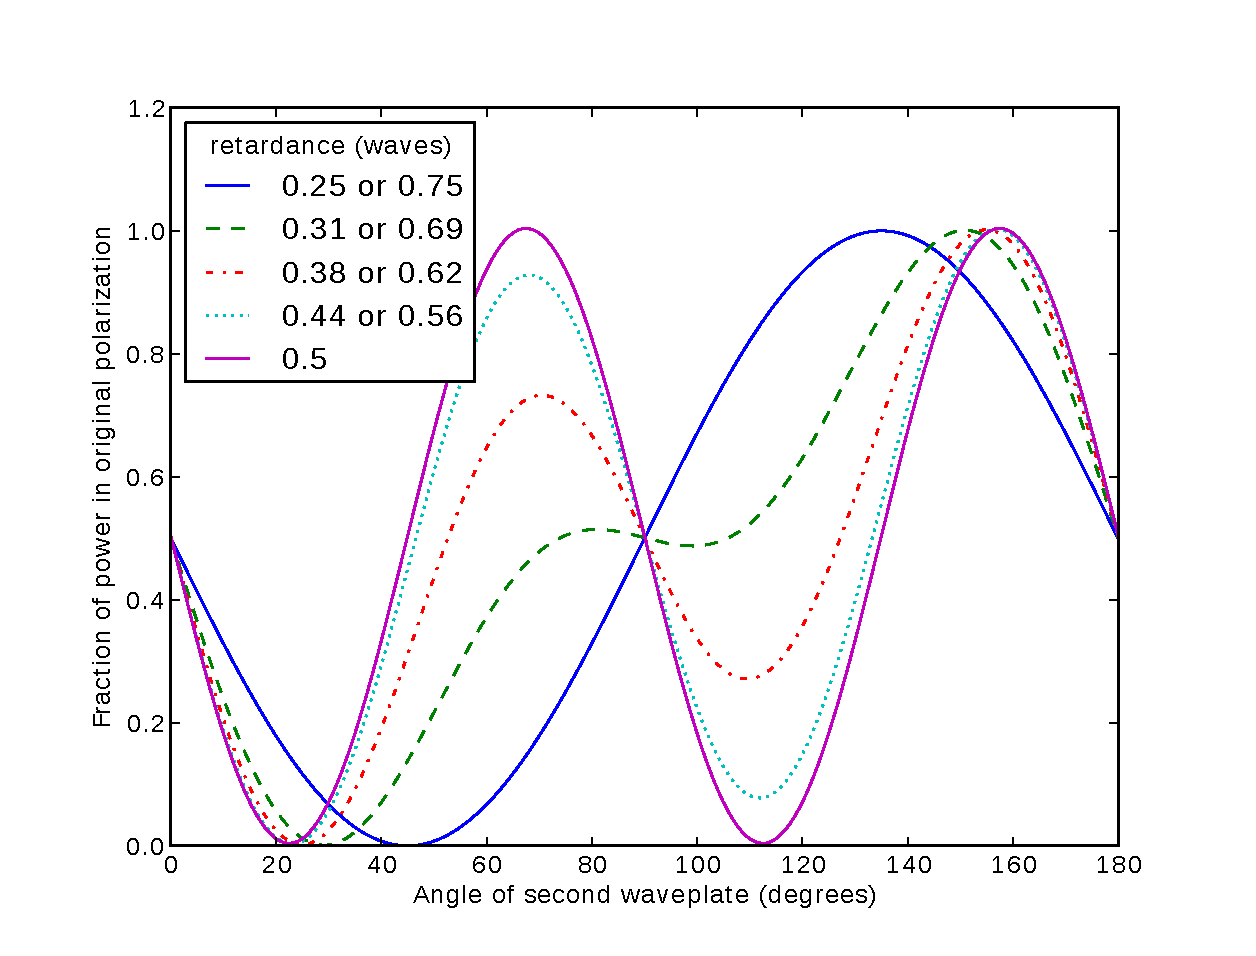
\includegraphics{NewNotesSymmetricFig}}
    \caption[Numerical method]{\label{fig:numericalLightControlMethod}
    A plot the magnitude of the fraction of the power at the original polarization as a function of the angle of the second waveplate for various retardances.}
\end{figure}


\section{Alignment Procedure}
By physical and numerical experimentation, we found that you can achieve these angles by subsequently adjusting each of the two waveplates in turn. Keeping 100\% of the light vertically polarized is easy and can be achieved for any fixed value of $\theta_2$ since $\theta_1$ can simply be adjusted so that the fast axis of the first waveplate aligns with the slow axis of the second. In this way, the total phase shift experienced by all the components is equal.

Thus, to correctly place the second waveplate at the angle  $\theta_2$, we adjust both angles until the outgoing light is entirely horizontally polarized (as measured by the output of the polarizing beam cube). I found that mounting the waveplates at the approximate angles I calculated followed by alternately adjusting each waveplate to minimize the amount of light transmitted achieved the desired result. 

\section{Results for other combinations of waveplates}
We performed additional numerical calculations and found a couple things:

This only works for certain retardances. If one of the waveplates has a retardance of 0.5 waves, then (obviously) this would work. If the two waveplates have the same retardance and that retardance is between 0.25 and 0.75 waves, this will also allow the user to put anywhere from 0\% to 100\% of the power into either polarization. Figure\,\ref{asymmetric} illustrates the maximum power that can be extinguished as a function of the retardance of the two waveplates.


\begin{figure}
    \centerline{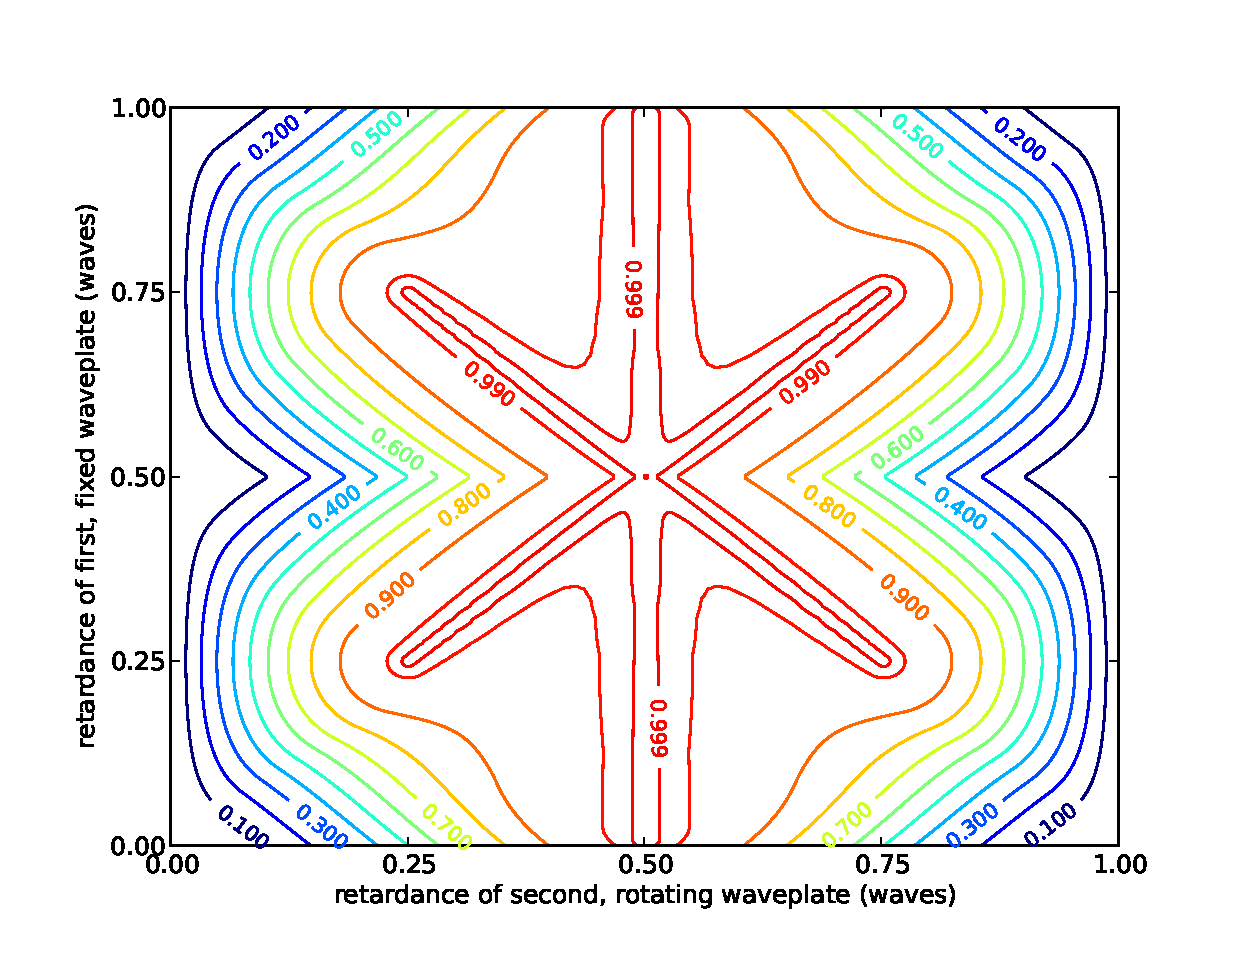
\includegraphics{NewNotesAsymmetricFigure}}
    \caption[Numerical method]{\label{asymmetric}
   The maximum power that one can extinguish through the polarizing beam cube given the retardance of the two waveplates. As one expects, if either waveplate has a retardance of 0.5 waves, one can get the full range of possible outgoing polarizations. However, this is only possible for certain combinations of waveplate retardances}
\end{figure}

\section{Attempt at building intuition}

Armed with the important clue that the we can use this trick only if the waveplates have the same retardance, we can make an attempt at describing the phenomenon only in terms of symmetry arguments.

We first consider vertically polarized light travelling into a waveplate. If we align the fast axis of the waveplate to the vertical direction, our vertically polarized light will emerge with a vertical polarization. 

However, if we rotate the fast axis to one side by some angle $\theta$, we get elliptically polarized light. Notice tht if we rotate the fast axis to the other side (i.e. by some angle $-\theta$) we also get elliptically polarized light. However, this light is elliptically polarized with the same ellipticity, but with the opposite handedness.

Now, we consider the second waveplate. We would like to consider what it would take to get horizontally polarized light coming out of the second waveplate. We can do this by noting that our system has time reversal symmetry. The time reversed outgoing horizontally polarized light turns out to be incoming horizontally polarized light. Similarly as before, the second waveplate can achieve elliptically polarized light of various handednesses.

Now, we simply argue that, by symmetry, we can place the two waveplates at some set of angles such that the elliptically polarized light coming out of the first waveplate corresponds to the time reversed elliptically polarized light coming through the second waveplate. It turns out that this leads to a nice symmetry in the result where, in order to get linearly polarized light out of the whole apparatus, the angle between the incoming polarization and the fast axis of the first waveplate will be equal in magnitude but opposite in sign to the angle between the outgoing polarization and the fast axis of the second waveplate.
%maybe do it differentially? You know? 

%let it be imperfect. Use other time for cleverness. Take advantage of having idea net out. 
%should I find a commutator? 
%IDK if I did this right with my \xi
%don't forget to cite peatrossware
%http://www.thorlabs.com/NewGroupPage9.cfm?ObjectGroup_ID=713 is where I got the spreadsheet. 

%  \include{AppendixB}

 \phantomsection \addcontentsline{toc}{chapter}{Index}
  \renewcommand{\baselinestretch}{1} \small \normalsize
  \printindex


\end{document}
